\chapter{Homology}
\section{Simplicial Homology}
\subsection{Simplicial Complexes}
If $S\sub\R^n$ is a linear subspace and $b\in\R^n$, the set
\[b+S=\{b+x:x\in S\}\]
is called an \textbf{affine subspace} of $\R^n$ parallel to $S$. We define the dimension of $b+S$ to be the dimension of $S$.\par
Suppose $v_0,\dots,v_k$ are $k+1$ distinct points in $\R^n$. As long as $n\geq k$, elementary linear algebra shows that there is always some $k$-dimensional affine subspace of $\R^n$ containing $\{v_0,\dots,v_k\}$: for example, if $S$ is any $k$-dimensional linear subspace containing $\{v_1-v_0,\dots,v_k-v_0\}$, then $v_0+S$ is such a space. We say that the set $\{v_0,\dots,v_k\}$ is \textbf{affinely independent} (or is \textbf{in general position}) if it is not contained in any affine subspace of dimension strictly less than $k$.
\begin{proposition}
For any $k+1$ distinct points $v_0,\dots,v_k\in\R^n$, the following are equivalent:
\begin{itemize}
\item[$(a)$] The set $\{v_0,\dots,v_k\}$ is affinely independent.
\item[$(b)$] The set $\{v_1-v_0,\dots,v_k-v_0\}$ is linearly independent.
\item[$(c)$] If $c_0,\dots,c_k$ are real numbers such that
\[\sum_{i=0}^{k}c_iv_i=0\And \sum_{i=0}^{k}c_i=0\]
then $c_0=\cdots=c_k=0$.
\end{itemize}
\end{proposition}
Let $\{v_0,\dots,v_k\}$ be an affinely independent set of $k+1$ points in $\R^n$. The simplex spanned by them, denoted by $[v_0,\dots,v_k]$, is the set
\[[v_0,\dots,v_k]:=\{\sum_{i=0}^{k}t_iv_i:t_i\geq 0\text{ and }\sum_{i=0}^{k}t_i=1\}\]
with the subspace topology. For any point $x=\sum_{i}t_iv_i\in[v_0,\dots,v_k]$, the numbers $t_i$ are called the \textbf{barycentric coordinates} of $x$ with respect to $[v_0,\dots,v_k]$. Each of the points $v_i$ is called a \textbf{vertex} of the simplex. The integer $k$ (one less than the number of vertices) is called its dimension; a $k$-dimensional simplex is often called a $k$-simplex.\par
For any subset $W\sub\R^n$, the convex hull of $W$ is defined to be the intersection of all convex sets containing $W$. It is immediate that the convex hull is itself a convex set, and in fact is the smallest convex set containing $W$.
\begin{proposition}
Every simplex is the convex hull of its vertices.
\end{proposition}
\begin{proposition}
Every $k$-simplex is a closed $k$-cell.
\end{proposition}
\begin{proof}
Consider first the standard $k$-simplex $\Delta^k=[e_0,\dots,e_k]\sub\R^k$ where $e_0=0$ and for $i=1,\dots,k$, $e_i=(0,\dots,1,\dots,0)$ has a $1$ in the $i$ th place and zeros elsewhere. This simplex is just the set of points $(t_1,\dots,t_k)\in\R^k$ such that $t_i\geq0$ for $i=1,\dots,k$ and $\sum_it_i\leq1$. Any point for which all these inequalities are strict is an
interior point, so $k$ is a closed $k$-cell by Proposition~\ref{CW compact convex is n-cell}.\par
Now suppose $\sigma=[v_0,\dots,v_k]\sub\R^n$ is an arbitrary $k$-simplex. Define a map $F:\Delta^k\to\sigma$ by $F(t_1,\dots,t_k)=t_0v_0+\cdots+t_kv_k$, where $t_0=1-\sum_{i=1}^{k}t_i$. This is a continuous bijection, and therefore a homeomorphism by the closed map lemma.
\end{proof}
Let $\sigma$ be a $k$-simplex. Each simplex spanned by a nonempty subset of the vertices of $\sigma$ is called a \textbf{face} of $\sigma$. The faces that are not equal to $\sigma$ itself are called its \textbf{proper faces}. The $0$-dimensional faces of $\sigma$ are just its vertices, and the $1$-dimensional faces are called its \textbf{edges}. The $(k-1)$-dimensional faces of a $k$-simplex are called
its \textbf{boundary faces}. Because $\sigma$ is a closed $k$-cell, it is a compact $k$-manifold with boundary.We define the \textbf{boundary} of $\sigma$ to be the union of its boundary faces (which is the same as the union of all of its proper faces, and is equal to its manifold boundary), and its \textbf{interior} to be $\sigma$ minus its boundary. An open $k$-simplex is the interior of a $k$-simplex. It consists of the set of points of the form $\sum_it_iv_i$, where $\{v_0,\dots,v_k\}$ are the vertices of the simplex, $\sum_it_i=1$, and all of the $t_i$'s are positive. For example, an open $0$-simplex is the same as a $0$-simplex, and an open $1$-simplex is a line segment minus its vertices. Note that unless $k=n$, an open $k$-simplex is not an open subset of $\R^n$, and its interior and boundary as a simplex are not equal to its topological interior and boundary as a subset of $\R^n$.\par
A (Euclidean) simplicial complex is a collection $K$ of simplices in some Euclidean
space $\R^n$, satisfying the following conditions:
\begin{itemize}
\item If $\sigma\in K$, then every face of $\sigma$ is in $K$.
\item The intersection of any two simplices in $K$ is either empty or a face of each.
\item $K$ is a locally finite collection.
\end{itemize}
The local finiteness condition implies that $K$ is countable, because every point of $\R^n$ has a neighborhood intersecting at most finitely many simplices of $K$, and this open cover of $\R^n$ has a countable subcover which must contains $K$. We are primarily concerned with finite simplicial complexes, which are those containing only finitely many simplices. For such complexes, condition $(\rmnum{3})$ is redundant.\par
If $K$ is a simplicial complex in $\R^n$, the dimension of $K$ is defined to be the
maximum dimension of the simplices in $K$; it is obviously no greater than $n$. A subset $K'\sub K$ is said to be a subcomplex of $K$ if whenever $\sigma\in K'$, every face of $\sigma$ is in $K'$. A subcomplex is a simplicial complex in its own right. For any $k\leq n$, the set of all simplices of $K$ of dimension at most $k$ is a subcomplex called the $k$-skeleton of $K$.\par
Given a simplicial complex $K$ in $\R^n$, the union of all the simplices in $K$, with the subspace topology inherited from $\R^n$, is a topological space denoted by $|K|$ and called the \textbf{polyhedron} of $K$.\par
The following observation is an easy consequence of the definitions.
\begin{proposition}
If $K$ is a Euclidean simplicial complex, then the collection consisting of the interiors of the simplices of $K$ is a regular CW decomposition of $|K|$.
\end{proposition}
\begin{remark}
Note that the cells in a CW decomposition are \textbf{open cells}, whereas the simplices of a simplicial complex are always understood to be \textbf{closed simplices}.
\end{remark}
\begin{example}\label{simplicial comp eg}
Here are some simple examples.
\begin{itemize}
\item[$(a)$] Any $n$-simplex together with all of its faces is a simplicial complex whose polyhedron is homeomorphic to $\widebar{\B}^n$.
\item[$(b)$] The set of proper faces of an $n$-simplex constitutes an $(n-1)$-dimensional
simplicial complex whose polyhedron is homeomorphic to $S^{n-1}$.
\item[$(c)$] For any integer $m\geq3$, let $P_m$ be a regular $m$-sided polygon in the plane. The set of edges and vertices of $P_m$ is a simplicial complex whose polyhedron is homeomorphic to $S^1$.
\item[$(d)$] We can construct a simplicial complex in $\R$ whose polyhedron is $\R$ itself: the $1$-simplices are the intervals $[n,n+1]$ for $n\in\Z$, and the $0$-simplices are the integers.
\item[$(e)$] Similarly, the set of all intervals $[n,n+1]$ for nonnegative integers $n$ together with their endpoints constitutes a simplicial complex in $\R$ whose polyhedron is $[0,\infty)$.
\end{itemize}
\end{example}
In general, if $X$ is a topological space, a homeomorphism between $X$ and the
polyhedron of some simplicial complex is called a \textbf{triangulation} of $X$. Any space that admits a triangulation is said to be \textbf{triangulable}. It follows from the classification theorem that all $1$-dimensional manifolds with and without boundary are triangulable.
\begin{theorem}[\textbf{Triangulation Theorem for $\bm{2}$-Manifolds}]\label{two mani triangulate}
Every $2$-manifold is homeomorphic to the polyhedron of a $2$-dimensional simplicial complex, in which every $1$-simplex is a face of exactly two $2$-simplices.
\end{theorem}
\begin{theorem}[\textbf{Triangulation Theorem for $\bm{3}$-Manifolds}]
Every $3$-manifold is triangulable.
\end{theorem}
\subsection{Simplicial Maps}
An \textbf{affine map} $F:\R^n\to\R^m$ is any map of the form $F(x)=c+A(x)$, where $A$ is a linear map and $c$ is some fixed vector in $\R^m$. Every affine map is continuous.
\begin{proposition}
Let $\sigma=[v_0,\dots,v_k]$ be a $k$-simplex in $\R^n$. Given any $k+1$ points
$w_0,\dots,w_k\in\R^m$, there is a unique map $f:\sigma\to\R^m$ that is the restriction of an affine map and takes $v_i$ to $w_i$ for each $i$.
\end{proposition}
\begin{proof}
we may assume that $v_0=0$ and $w_0=0$. Under this assumption, the set $\{v_1,\dots,v_k\}$ is linearly independent, so we can let $f:\sigma\to\R^m$ be the restriction of any linear map such that $f(v_i)=w_i$ for $i=1,\dots,v_k$.\par
A straightforward computation shows that if $f:\sigma\to\R^m$ is the restriction of any affine map, then it satisfies
\[f\Big(\sum_{i=0}^{k}t_iv_i\Big)=\sum_{i=0}^{k}t_if(v_i)\]
when applied to points in $\sigma$. This shows that $f$ is uniquely determined by where it sends the vertices of $\sigma$.
\end{proof}
In the situation of the preceding proposition, we say that the map $f:\sigma\to\R^m$ is the \textbf{affine map determined by the vertex map} $v_i\mapsto w_i$, $i=1,\dots,k$.\par
This construction leads to a natural notion of maps between simplicial complexes.
Suppose $K$ and $L$ are simplicial complexes, and let $K_0$ and $L_0$ denote their
respective $0$-skeleta (i.e., their sets of vertices). A \textbf{simplicial map} from $K$ to $L$ is a continuous map $f:|K|\to|L|$ whose restriction to each simplex $\sigma\in K$ agrees with an affine map taking $\sigma$ onto some simplex in $L$. The restriction of $f$ to $K_0$ yields a map $f_0:K_0\to L_0$ called the \textbf{vertex map} of $f$. A simplicial map is called a simplicial isomorphism if it is also a homeomorphism; in this case, it is easy to check that the inverse of $f$ is also a simplicial map. The central reason why we study simplicial complexes is contained in the following theorem.
\begin{theorem}\label{simplical map}
Let $K$ and $L$ be simplicial complexes. Suppose $f_0:K_0\to L_0$ is any map with the property that whenever $\{v_0,\dots,v_k\}$ are the vertices of a simplex of $K$, $\{f(v_0),\dots,f(v_k)\}$ are the vertices of a simplex of $L$ $($possibly with repetitions$)$. Then there is a unique simplicial map $f:|K|\to|L|$ whose vertex map is $f_0$. It is a simplicial isomorphism if and only if $f_0$ is a bijection satisfying the following additional condition: $\{v_0,\dots,v_k\}$ are the vertices of a simplex of $K$ if and only if $\{f(v_0),\dots,f(v_k)\}$ are
the vertices of a simplex of $L$.
\end{theorem}
\subsection{Abstract Simplicial Complexes}
Theorem~\ref{simplical map} says that a simplicial complex is completely determined up to simplicial isomorphism by knowledge of its vertices and which sets of vertices span simplices. Motivated by this observation, we define an \textbf{abstract simplicial complex} to be a collection $\mathcal{K}$ of nonempty finite sets, subject to only one condition: if $s\in\mathcal{K}$, then every nonempty subset of $s$ is in $\mathcal{K}$.\par
If $\mathcal{K}$ is an abstract simplicial complex, the finite sets that make up $\mathcal{K}$ are called \textbf{abstract simplices}. Given an abstract simplex $s\in\mathcal{K}$, any element of $s$ is called a \textbf{vertex} of $s$, and any nonempty subset of $s$ is called a \textbf{face} of $s$. We say $\mathcal{K}$ is a \textbf{finite complex} if $\mathcal{K}$ itself is a finite set, and a \textbf{locally finite complex} if every vertex belongs to only finitely many abstract simplices. The \textbf{dimension of an abstract simplex} $s\in\mathcal{K}$ is one less than the number of elements of $s$. If the dimensions of the abstract simplices of $\mathcal{K}$ are bounded above, then we say $\mathcal{K}$ is \textbf{finite-dimensional}, and its dimension is the smallest upper bound of the dimensions of its simplices.\par
Now suppose that $\mathcal{K}$ and $\mathcal{L}$ are abstract complexes. Define their vertex sets by
\[\mathcal{K}_0=\bigcup_{s\in\mathcal{K}}s,\quad \mathcal{L}_0=\bigcup_{s\in\mathcal{L}}s.\]
A map $f:\mathcal{K}\to\mathcal{L}$ is called an \textbf{abstract simplicial map} if it is of the form $f(\{v_0,\dots,v_k\})=\{f_0(v_0),\dots,f_0(v_k)\}$ for some map $f_0:\mathcal{K}_0\to\mathcal{L}_0$, called the \textbf{vertex map} of $f$ (which must have the property that $\{f_0(v_0),\dots,f_0(v_k)\}$ whenever $\{v_0,\dots,v_k\}\in\mathcal{K}$). An abstract simplicial map $f$ is called an isomorphism if both $f_0$ and $f$ are bijections. In that case, $f^{-1}$ is also an abstract simplicial map.\par
One way of constructing an abstract simplicial complex, as you have probably
already guessed, is the following. Given a Euclidean simplicial complex $K$, let $\mathcal{K}$ denote the collection of all those finite sets $\{v_0,\dots,v_k\}$ that consist of the vertices of some simplex of $K$. It is immediate that $\mathcal{K}$ is an abstract simplicial complex, called the vertex scheme of $K$. It follows from Theorem~\ref{simplical map} that two Euclidean complexes are simplicially isomorphic if and only if their vertex schemes are isomorphic.
We can also start with an abstract simplicial complex $\mathcal{K}$ and attempt to go back the other way. If $K$ is a Euclidean simplicial complex whose vertex scheme is isomorphic to $\mathcal{K}$, we say $K$ is a \textbf{geometric realization} of $\mathcal{K}$. The discussion above shows that $K$ is uniquely determined by $\mathcal{K}$, up to simplicial isomorphism. As the next proposition shows, constructing a geometric realization in the finite case is easy.
\begin{proposition}
Every finite abstract simplicial complex has a geometric realization.
\end{proposition}
\begin{proof}
Let $v_1,\dots,v_m$ be the vertices of $\mathcal{K}$ in some order, and let $K\sub\R^m$ be the complex whose vertices are the points $\{e_1,\dots,e_m\}$, where $e_i=(0,\dots,1,\dots,0)$, with simplices $[e_{i_1},\dots,e_{i_k}]\in K$ if and only if $\{v_{i_1},\dots,v_{i_k}\}$. Since all these simplices are faces of the standard $m$-simplex $\Delta^m$, the intersection condition is satisfied,
and it is straightforward to show that the vertex scheme of $K$ is isomorphic
to $\mathcal{K}$.
\end{proof}
\begin{example}
The following abstract complexes
are isomorphic to the vertex schemes of the Euclidean complexes of Example~\ref{simplicial comp eg}:
\begin{itemize}
\item[$(a)$] The set of all nonempty subsets of $\{0,1,\dots,n\}$ is an abstract complex whose geometric realization is homeomorphic to $\widebar{\B}^n$.
\item[$(b)$] The set of all proper nonempty subsets of $\{0,1,\dots,n\}$ is an abstract complex whose geometric realization is homeomorphic to $S^{n-1}$.
\item[$(c)$] Let $m$ be an integer greater than or equal to $3$, and let $K_m$ be the abstract complex whose $0$-simplices are $\{\{1\},\{2\},\dots,\{n\}\}$, and whose $1$-simplices are $\{\{1,2\},\{2,3\},\dots,\{m-1,m\},\{m,1\}\}$. Its geometric realization is homeomorphic to $S^1$.
\item[$(d)$] The set $\mathcal{R}$ of all singletons $\{n\}$ and all pairs of the form $\{n,n+1\}$ as $n$ ranges over the integers, is an abstract complex that has a geometric realization homeomorphic to $\R$.
\item[$(e)$] The subset of $\mathcal{R}$ consisting of those singletons $\{n\}$ and pairs $\{n,n+1\}$ for which $n\geq 0$ is an abstract complex that has a geometric realization homeomorphic to $[0,\infty)$.
\end{itemize}
\end{example}
The most natural way to modify a simplicial complex to obtain another one with a homeomorphic polyhedron is to \textit{subdivide} the simplices of the original complex into smaller ones. If $K$ is a Euclidean simplicial complex,
a subdivision of $K$ is a simplicial complex $K'$ such that each simplex of $K'$ is contained in a simplex of $K$, and each simplex of $K$ is a union of simplices of $K'$. It follows immediately from these properties that $|K|=|K'|$.
\subsection{\boldmath$\Delta$-Complex}
The torus, the projective plane, and the Klein bottle can each be obtained from a square by identifying opposite edges in the way indicated by the arrows in the following figures:
\[\includegraphics[width=0.8\textwidth]{delta-complex.pdf}\]
Cutting a square along a diagonal produces two triangles, so each of these surfaces can also be built from two triangles by identifying their edges in pairs. In similar fashion a polygon with any number of sides can be cut along diagonals into triangles, so in fact all closed surfaces can be constructed from triangles by identifying edges.\par
We begin with some definitions. For any integer $n\geq0$, let $\Delta^n\sub\R^n$ denote the \textbf{standard $\bm{n}$-simplex} $[e_0,\dots,e_n]$. The union of all the faces of $\Delta^n$ is the boundary of $\Delta^n$, written $\partial\Delta^n$. The open simplex $\Int(\Delta^n)$ is $\Delta^n-\partial\Delta^n$, the interior of $\Delta^n$.\par
A \textbf{$\bm{\Delta}$-complex} structure on a space $X$ is a collection of maps $\sigma_\alpha:\Delta^n\to X$, with $n$ depending on the index $\alpha$, such that:
\begin{itemize}
\item[$(\rmnum{1})$]The restriction $\sigma_\alpha|_{\Int(\Delta^n)}$ is injective, and each point of $X$ is in the image of exactly
one such restriction $\sigma_\alpha|_{\Int(\Delta^n)}$.
\item[$(\rmnum{2})$]Each restriction of $\sigma_\alpha$ to a face of $\Delta^n$ is one of the maps $\sigma_\beta:\Delta^{n-1}\to X$. Here we are identifying the face of $\Delta^n$ with $\Delta^{n-1}$ by the canonical linear homeomorphism between them that preserves the ordering of the vertices.
\item[$(\rmnum{3})$]A set $A\sub X$ is open iff $\sigma^{-1}_\alpha(A)$ is open in $\Delta^n$ for each $\sigma_\alpha$.
\end{itemize}
Among other things, this last condition rules out trivialities like regarding all the points of $X$ as individual vertices. The earlier decompositions of the torus, projective plane, and Klein bottle into two triangles, three edges, and one or two vertices define $\Delta$-complex structures with   total of six $\sigma_\alpha$'s for the torus and Klein bottle and seven for the projective plane. The orientations on the edges in the pictures are compatible with a unique ordering of the vertices of each simplex, and these orderings determine the maps $\sigma_\alpha$.\par
A consequence of $(\rmnum{3})$ is that $X$ can be built as a quotient space of a collection of disjoint simplices $\Delta^n_\alpha$, one for each $\sigma_\alpha:\Delta^n\to X$, the quotient space obtained by identifying each face of a $\Delta^n_\alpha$ with the $\Delta_\beta^{n-1}$ corresponding to the restriction $\sigma_\beta$ of $\sigma_\alpha$ to the face in question, as in condition $(\rmnum{2})$. One can think of building the quotient space inductively, starting with a discrete set of vertices, then attaching edges to
these to produce a graph, then attaching $2$-simplices to the graph, and so on. From this viewpoint we see that the data specifying a $\Delta$-complex can be described purely combinatorially as collections of $n$-simplices $\Delta^n_\alpha$ for each $n$ together with functions associating to each face of each $n$ simplex $\Delta^n_\alpha$ an $(n-1)$ simplex $\Delta^{n-1}_\beta$.\par
Thinking of a $\Delta$-complex $X$ as a quotient space of a collection of disjoint simplices, it is not hard to see that $X$ must be a Hausdorff space. Condition $(\rmnum{3})$ then implies that each restriction $\sigma_\alpha|_{\Int(\Delta^n)}$ is a homeomorphism onto its image, which is
thus an open simplex in $X$. It follows from Proposition~\ref{CW maps are char map iff} that these open simplices $\sigma_\alpha(\Int(\Delta^n))$ are the cells 
$e^n_\alpha$ of a CW complex structure on $X$ with the $\sigma_\alpha$'s as characteristic maps.
\subsection{Simplicial Homology Groups}
Our goal now is to define the simplicial homology groups of a $\Delta$-complex $X$. Let $\Delta^n(X)$ be the free abelian group with basis the open $n$-simplices $e^n_\alpha$ of $X$. Elements of $\Delta_n(X)$, called $n$ chains, can be written as finite formal sums $\sum_\alpha n_\alpha e^n_\alpha$ with coefficients $n_\alpha\in\Z$. Equivalently, we could write $\sum_\alpha n_\alpha\sigma_\alpha$ where $\sigma_\alpha:\Delta^n\to X$ is the
characteristic map of $e^n_\alpha$, with image the closure of $e^n_\alpha$ as described above. Such a sum $\sum_\alpha n_\alpha\sigma_\alpha$ can be thought of as a finite collection, or chain, of $n$-simplices in $X$ with integer multiplicities, the coefficients $n_\alpha$.\par
With this geometry in mind we define for a general $\Delta$-complex $X$ a boundary homomorphism $\partial_n:\Delta_n(X)\to\Delta_{n-1}(X)$ by specifying its values on basis elements:
\[\partial_n(\sigma_\alpha)=\sum_i(-1)^i\sigma_\alpha[v_0,\dots,\widehat{v}_i,\dots,v_m].\]
Note that the right side of this equation does indeed lie in $\Delta_{n-1}(X)$ since each restriction $\sigma_\alpha[v_0,\dots,\widehat{v}_i,\dots,v_m]$ is the characteristic map of an $(n-1)$ simplex of $X$.\par
\begin{lemma}
The composition 
\[\begin{tikzcd}
\Delta_n(X)\ar[r,"\partial_n"]&\Delta_{n-1}(X)\ar[r,"\partial_{n-1}"]&\Delta_{n-2}(X)
\end{tikzcd}\]
is zero.
\end{lemma}
The algebraic situation we have now is a sequence of homomorphisms of abelian
groups
\[\begin{tikzcd}
\cdots\ar[r]&\Delta_{n+1}(X)\ar[r,"\partial_{n+1}"]&\Delta_{n}(X)\ar[r,"\partial_{n}"]&\Delta_{n-1}(X)\ar[r,"\partial_{n-1}"]&\cdots
\end{tikzcd}\]
The homology group $\ker\partial_n/\im\partial_{n+1}$ will be denoted $H^\Delta_n(X)$ and called the nth simplicial homology group of $X$.
\begin{example}
$X=S^1$, with one vertex $v$ and one edge $e$. 
\[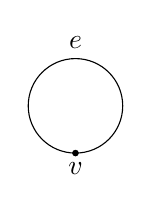
\begin{tikzpicture}[scale=0.6]
\draw (0,1) circle [radius=1];
\node [above] at (0,2) {$e$};
\node (v) [below,dotted] at (0,0) {$v$};
\fill[black] (0,0) circle (2pt);
\end{tikzpicture}\]
Then $\Delta_0(S^1)$ and $\Delta_1(S^1)$ are both $\Z$ and the boundary map $\partial_1$ is zero since $\partial e=v-v$. The groups $\Delta_n(S^1)$ are $0$ for $n\geq2$ since there are no simplices in these dimensions. Hence
\[H_n^\Delta(S^1)=\begin{cases}
\Z&\text{for }n=0,1;\\
0&\text{for }n\geq 2.
\end{cases}\]
This is an illustration of the general fact that if the boundary maps in a chain complex are all zero, then the homology groups of the complex are isomorphic to the chain groups themselves.
\end{example}
\begin{example}
$X=T$, the torus with the $\Delta$-complex structure pictured earlier, having one vertex, three edges $a$, $b$, and $c$, and two $2$-simplices $U$ and $L$. As in the previous example, $\partial_1=0$ so $H^\Delta_0(T)=\Z$. Since $\partial_2U=a+b-c=\partial_2L$ and $\{a,b,a+b-c\}$ is a basis for $\Delta_1(T)$, it follows that $H^\Delta_1(T)=\Z\oplus\Z$ with basis the homology classes $[a]$ and $[b]$. Since there are no $3$-simplices, $H^\Delta_2(T)$ is equal to $\ker\partial_2$, which is infinite cyclic generated by $U-L$ since $\partial(pU+qL)=(p+q)(a+b-c)=0$ only if $p=-q$. Thus
\[H_n^\Delta(T)=\begin{cases}
\Z\oplus\Z&\text{for }n=1;\\
\Z&\text{for }n=0,2;\\
0&\text{for }n\geq 3.
\end{cases}\]
\end{example}
\begin{example}
$X=\RP^2$, as pictured earlier, with two vertices $v$ and $w$, three edges $a$, $b$, and $c$, and two $2$-simplices $U$ and $L$. Then 
\[\left\{\begin{array}{l}
\partial_1(pa+qb+sc)=p(w-v)+q(w-v)=(p+q)(w-v);\\
\partial_2(pU+qL)=p(c+b-a)+q(c+a-b)=(q-p)(a-b)+(q+p)c.
\end{array}\right. \]
Then $\im\partial_1$ is generated by $w-v$, so $H^\Delta_0(X)=\Z$ with either vertex as a generator. Since we see that $\partial_2$ is injective, $H^\Delta_2(X)=0$. Further, $\ker\partial_1$ has basis $(a-b)$ and $c$, while $\im\partial_2$ can be written as
\[(q-p)(a-b)+(q+p)c=t(a-b)+(t+2p)c=t(a-b+c)+p(2c).\]
So it an index-two subgroup of $\ker\partial_1$, and we have $H^\Delta_1(X)=\Z/2\Z$.
\[H_n^\Delta(\RP^2)=\begin{cases}
\Z&\text{for }n=0;\\
\Z/2\Z&\text{for }n=1;\\
0&\text{for }n\geq 2.
\end{cases}\]
\end{example}
\begin{example}
$X=K$, as pictured earlier, with one vertex $v$, three edges $a$, $b$, and $c$, and two $2$-simplices $U$ and $L$. We have
\[\left\{\begin{array}{l}
\partial_1=0;\\
\partial_2(pU+qL)=p(a+b-c)+q(a-b+c)=(p+q)a+(p-q)(b-c).
\end{array}\right. \]
It follows that $H_0^\Delta(X)=\Z$, and $H^\Delta_2(X)=0$ since $\partial_2$ is injective. Now we can choose basis $a+b-c$ and $2(b-c)$ for $\im\partial_2$ as in the previous example, so $\im\partial_2$ is a subgroup of index $2$. Then $H^\Delta_1(X)=\Z\oplus\Z/2\Z$. 
\[H_n^\Delta(K)=\begin{cases}
\Z&\text{for }n=0;\\
\Z\oplus\Z/2\Z&\text{for }n=1;\\
0&\text{for }n\geq 2.
\end{cases}\]
\end{example}
\begin{example}
We can obtain a $\Delta$-complex structure on $S^n$ by taking two copies of $\Delta^n$ and identifying their boundaries via the identity map. Labeling these two $n$-simplices $U$ and $L$, then it is obvious that $\ker\partial_n$ is infinite cyclic generated by $U-L$. Thus $H^\Delta_n(S^n)=\Z$ for this $\Delta$-complex structure on $S^n$. Computing the other homology groups would be more difficult.
\end{example}
\section{Singular Homology}
\subsection{Singular Homology Groups}
 If $X$ is a topological space, a \textbf{singular $\bm{p}$-simplex} in $X$ is a continuous map $\sigma:\Delta^p\to X$. (A map is generally called \textit{singular} if it fails to have some desirable property such as continuity or differentiability. In this case, the term singular is meant to reflect the fact that $\sigma$ need not be
an embedding, so its image might not look at all like a simplex.)\par
Let $C_p(X)$ be the free abelian group on the set of all singular $p$-simplices in $X$. An element of $C_p(X)$, which can be written as a formal linear combination of singular simplices with integer coefficients, is called a \textbf{singular $\bm{p}$-chain} in $X$, and the group $C_p(X)$ is called the \textbf{singular chain group} in dimension $p$.\par
There are some special singular simplices in Euclidean spaces that we use frequently. Let $K\sub\R^n$ be a convex subset. For any $p+1$ points $v_0,\dots,v_p\in K$ (not necessarily affinely independent or even distinct), let $A(v_0,\dots,v_p):\Delta^p\to\R^n$ denote
the affine map that takes $e_i$ to $v_i$ for $i=0,\dots,p$. By convexity, the image lies in $K$, so this is a singular $p$-simplex in $K$, called an \textbf{affine singular simplex}. A singular chain in which every singular simplex that appears is affine is called an \textbf{affine chain}.\par
We define a homomorphism from $p$-chains to $p-1$-chains that precisely captures the notion of boundary values. For each $i=0,\dots,p$, let $F_{i,p}:\Delta_{p-1}\to\Delta_{p}$ be the affine singular simplex
\[F_{i,p}=A(e_0,\dots,\widehat{e}_i,\dots,e_p).\]
More specifically, $F_{i,p}$ is the affine map that sends
\[e_0\mapsto e_0,\ \cdots,\ e_{i-1}\mapsto e_{i-1},\ e_i\mapsto e_{i+1},\ \cdots,\ e_{p-1}\mapsto e_p.\]
and therefore maps $\Delta_{p-1}$ homeomorphically onto the boundary face of $\Delta^p$ opposite the vertex $e_i$. We call $F_{i,p}$ the $i$ th \textbf{face map} in dimension $p$.\par
For any singular simplex $\sigma:\Delta^p\to X$, define a $(p-1)$-chain $\partial\sigma$ called the boundary of $\sigma$ by
\[\partial\sigma=\sum_{i=0}^{p}(-1)^p\sigma\circ F_{i,p}=\sum_{i=0}^{p}(-1)^p\sigma[e_0,\dots,\widehat{e}_j,\dots,e_p].\]
By the universal property of free abelian groups, this extends uniquely to a homomorphism $\partial:C_p(X)\to C_{p-1}(X)$, called the \textbf{singular boundary operator}. We sometimes indicate which chain group the boundary operator is acting on by a subscript, as in $\partial_p:C_p(X)\to C_{p-1}(X)$. The boundary of any $0$-chain is defined to be zero.\par
A $p$-chain $c$ is called a \textbf{cycle} if $\partial c=0$, and it is called a \textbf{boundary} if there exists a $(p+1)$-chain $b$ such that $c=\partial b$. The set $Z_p(X)$ of $p$-cycles is a subgroup of $C_p(X)$, because it is the kernel of the homomorphism $\partial_p$. Similarly, the set $B_p(X)$ of $p$-boundaries is also a subgroup (the image of $\partial_{p+1}$).\par
The most important feature of the singular boundary map is that \textit{the boundary of a boundary is zero}, as the next lemma shows.
\begin{lemma}
If $c$ is a singular chain, then $\partial^2c=0$.
\end{lemma}
We compute
\begin{align*}
\partial^2c&=\sum_{j=0}^{i-1}\sum_{i=1}^{p}(-1)^{i+j}\sigma[e_0,\dots,\widehat{e}_j,\dots,\widehat{e}_i,\dots,e_p]+\sum_{j=i+1}^{p}\sum_{i=0}^{p}(-1)^{i+j-1}\sigma[e_0,\dots,\widehat{e}_i,\dots,\widehat{e}_j,\dots,e_p]\\
&=\sum_{j=0}^{i-1}\sum_{i=1}^{p}(-1)^{i+j}\sigma[e_0,\dots,\widehat{e}_j,\dots,\widehat{e}_i,\dots,e_p]-\sum_{i=j+1}^{p}\sum_{j=0}^{p}(-1)^{i+j}\sigma[e_0,\dots,\widehat{e}_j,\dots,\widehat{e}_i,\dots,e_p]\\
&=\sum_{j=0}^{i-1}\sum_{i=1}^{p}(-1)^{i+j}\sigma[e_0,\dots,\widehat{e}_j,\dots,\widehat{e}_i,\dots,e_p]-\sum_{j=0}^{i-1}\sum_{i=1}^{p}(-1)^{i+j}\sigma[e_0,\dots,\widehat{e}_j,\dots,\widehat{e}_i,\dots,e_p]\\
&=0.
\end{align*}
Because of the preceding lemma, the group $B_p(X)$ of $p$-boundaries is a subgroup of the group $Z_p(X)$ of $p$-cycles. The $p$-th singular homology group of $X$ is defined to be the quotient group
\[H_p(X)=\dfrac{Z_p(X)}{B_p(X)}=\dfrac{\ker\partial_p}{\im\partial_{p+1}}.\]
The equivalence class of a $p$-cycle $c$ in $H_p(X)$ is denoted by $[c]$, and is called its homology class. If two $p$-cycles determine the same homology class (i.e., if they differ by a boundary), they are said to be \textbf{homologous}.\par
Given a continuous map $f:X\to Y$, let $f_{\sharp}:C_p(X)\to C_p(Y)$ be the homomorphism defined by setting $f_{\sharp}\sigma=f\circ\sigma$ for each singular $p$-simplex $\sigma$. The key fact is that $f_{\sharp}$ commutes with the boundary operators:
\[f_{\sharp}(\partial\sigma)=\sum_{i=0}^{p}(-1)^if\circ\sigma\circ F_{i,p}=\partial(f_{\sharp}\sigma).\]
Because of this, $f_\sharp$ maps $Z_p(X)$ to $Z_p(Y)$ and $B_p(X)$ to $B_p(Y)$, and therefore passes to the quotient to define a homomorphism $f_{*}:H_p(X)\to H_p(Y)$, 
called the \textbf{homomorphism induced by $\bm{f}$}.
\begin{proposition}[\textbf{Functorial Properties of Homology}]
Let $X$, $Y$, and $Z$ be topological spaces.
\begin{itemize}
\item[$(a)$]The homomorphism $(\id)_*:H_p(X)\to H_p(X)$ induced by the identity map of $X$ is the identity of $H_p(X)$.
\item[$(b)$]If $f:X\to Y$ and $g:Y\to Z$ are continuous maps, then
\[(g\circ f)_*=g_*\circ f_*.\]
\end{itemize}
Thus the pth singular homology group defines a \textbf{covariant functor} from the category of topological spaces to the category of abelian groups.
\end{proposition}
\begin{corollary}[\textbf{Topological Invariance of Singular Homology}]
If $f:X\to Y$ is a homeomorphism, then $f_*:H_p(X)\to H_p(Y)$ is an isomorphism.
\end{corollary}
\begin{corollary}[\textbf{Homology of a Retract}]
Suppose $X$ is a topological space and $A\sub X$ is a retract of $X$. Then for each $p$, the homology homomorphism $H_p(A)\to H_p(X)$ induced by inclusion is injective.
\end{corollary}
\subsection{Exact Sequences and Chain Complexes}
More generally, a sequence of abelian groups and homomorphisms
\[\begin{tikzcd}
\cdots\ar[r]&C_{p+1}\ar[r,"\partial_{p+1}"]&C_p\ar[r,"\partial_p"]&C_{p-1}\ar[r]&\cdots
\end{tikzcd}\]
is called a chain complex if the composition of any two consecutive homomorphisms is the zero map: $\partial_{p+1}\circ\partial_p=0$. We denote such a complex by $C_\bullet$. The $p$-th \textbf{homology group} of the chain complex $C_\bullet$ is
\[H_p(C_\bullet)=\dfrac{\ker\partial_{p}}{\im\partial_{p+1}}.\]
The chain complex is exact if and only if $H_p(C_\bullet)=0$ for all $p$; thus the homology groups provide a precise quantitative measurement of the \textit{failure of exactness}.\par
Now suppose $C_\bullet$ and $D_\bullet$ are chain complexes. A chain map $F:C_\bullet\to D_\bullet$ is a collection of homomorphisms $F:C_p\to D_p$ (we could distinguish them with subscripts, but there is no need) such that $\partial_p\circ F=F\circ\partial_p$ for all $p$:
\[\begin{tikzcd}
\cdots\ar[r]&C_{p+1}\ar[d,"F"]\ar[r,"\partial_{p+1}"]&C_p\ar[d,"F"]\ar[r,"\partial_p"]&C_{p-1}\ar[d,"F"]\ar[r]&\cdots\\
\cdots\ar[r]&D_{p+1}\ar[r,"\partial_{p+1}"]&D_p\ar[r,"\partial_p"]&D_{p-1}\ar[r]&\cdots
\end{tikzcd}\]
For example, the homomorphisms $f_\sharp:C_p(X)\to C_p(Y)$ constructed above from a continuous map $f$ define a chain map from the singular chain complex of $X$ to that of $Y$. Any chain map takes $\ker\partial$ to $\ker\partial$ and $\im\partial$ to $\im\partial$, and therefore induces a homology homomorphism $F_*:H_p(X)\to H_p(Y)$ for each $p$.
\subsection{Elementary Computations}
\begin{proposition}\label{component homology}
Let $X$ be a space, let $\{X_\alpha\}_{\alpha\in A}$ be the set of path components of $X$, and let $\iota_\alpha:X_\alpha\to X$ be inclusion. Then for each $p\geq0$ the map
\[\bigoplus_{\alpha\in A}H_p(X_\alpha)\to H_p(X),\]
whose restriction to $H_p(X_\alpha)$ is $(\iota_\alpha)_*:H_p(X_\alpha)\to H_p(X)$, is an isomorphism.
\end{proposition}
\begin{proof}
Since the image of any singular simplex must lie entirely in one path component, the chain maps $(\iota_\alpha)_\sharp:C_p(X_\alpha)\to C_p(X)$ already induce isomorphisms
\[\bigoplus_{\alpha\in A}C_p(X_\alpha)\to C_p(X).\]
The result for homology follows easily from this.
\end{proof}
\begin{proposition}[\textbf{Zero-Dimensional Homology}]\label{homology 0 dim}
For any topological space $X$, $H_0(X)$ is a free abelian group with basis consisting of an arbitrary point in each path component.
\end{proposition}
\begin{proof}
It suffices to show that $H_0(X)$ is the infinite cyclic group generated by the class of any point when $X$ is path-connected, for then in the general case Proposition~\ref{component homology} guarantees that $H_0(X)$ is the direct sum of infinite cyclic groups, one for each path component.\par
A singular $0$-chain is a formal linear combination of points in $X$ with integer coefficients: $c=\sum_{i=1}^{m}n_ix_i$. Because the boundary operator is the zero map in dimension $0$, every $0$-chain is a cycle.\par
Assume that $X$ is path-connected, and define a map $\eps:C_0(X)\to\Z$ by
\[\eps\Big(\sum_{i=1}^{m}n_ix_i\Big)=\sum_{i=1}^{m}n_i.\]
It is immediate from the definition that $\eps$ is a surjective homomorphism. We will show that $\ker\eps=B_0(X)$, from which it follows by the first isomorphism theorem that $\eps$ induces an isomorphism $H_0(X)\to\Z$. Since $\eps$ takes any single point to $1$, the result follows.\par
If $\sigma$ is a singular $1$-simplex, then $\partial\sigma=\sigma(1)-\sigma(0)$, so $\eps(\partial\sigma)=1-1=0$. Therefore, $B_0(X)\sub\ker\eps$. To show that $\ker\eps\sub B_0(X)$, choose any point $x_0\in X$, and for each $x\in X$ let $\alpha(x)$ be a path from $x_0$ to $x$. This is a singular $1$-simplex whose boundary is the $0$-chain $x-x_0$. Thus, for an arbitrary $0$-chain $c=\sum_{i=1}n_ix_i$ we compute
\[\partial\Big(\sum_in_i\alpha_i(x_i)\Big)=\sum_in_ix_i-\sum_in_ix_0=c-\eps(c)x_0.\]
In particular, if $\eps(c)=0$, then $c\in B_0(X)$.
\end{proof}
\begin{proposition}[\textbf{Homology of a Discrete Space}]\label{homology point}
If $X$ is a discrete space, then $H_0(X)$ is a free abelian group with one generator for each point of $X$, and $H_p(X)=0$ for $p>0$.
\end{proposition}
\begin{proof}
The case $p=0$ follows from the preceding proposition, so we concentrate
on $p>0$. By Proposition~\ref{component homology}, it suffices to show that $H_p(\ast)=0$ when $\ast$ is a one-point space. In that case, there is exactly one singular simplex in each dimension, namely the constant map $\sigma_p:\Delta^p\to\ast$, so each chain group $C_p(\ast)$ is the infinite cyclic group generated by $\sigma_p$. For $p>0$, the boundary of $\sigma_p$ is the alternating sum
\[\partial\sigma_p=\sum_{i=0}^{p}(-1)^i\sigma\circ F_{i,p}=\sum_{i=0}^{p}(-1)^i\sigma_{p-1}=\begin{cases}
0&p\text{ is odd};\\
\sigma_{p-1}&p\text{ is even}.
\end{cases}\]
Thus $\partial:C_p(\ast)\to C_{p-1}(\ast)$ is an isomorphism when $p$ is even and positive, and the zero map when $p$ is odd:
\[\begin{tikzcd}
\cdots\ar[r,"\cong"]&C_3(\ast)\ar[r,"0"]&C_2(\ast)\ar[r,"\cong"]&C_1\ar[r,"0"]&C_0(\ast)\ar[r]&0
\end{tikzcd}\]
This sequence is exact at each group except the last, so $H_p(\ast)=0$ for $p>0$.
\end{proof}
It is often very convenient to have a slightly modified version of homology for which a point has trivial homology groups in all dimensions, including zero. This is done by defining the \textbf{reduced homology groups} $\widetilde{H}_p(X)$ to be the homology groups of the augmented chain complex
\[\begin{tikzcd}
\cdots\ar[r]&C_2(X)\ar[r,"\partial_2"]&C_1(X)\ar[r,"\partial_1"]&C_0(X)\ar[r,"\eps"]&\Z\ar[r]&0
\end{tikzcd}\]
where $\eps(\sum_in_ix_i)=\sum_in_i$ as in the proof of Proposition~\ref{homology 0 dim}. Here we had better
require $X$ to be nonempty, to avoid having a nontrivial homology group in dimension $-1$. Since $\eps\partial_1=0$, $\eps$ vanishes on $\im\partial_1$ and hence induces a map 
\[H_0(X)=\dfrac{C_0(X)}{\im\partial_1}\stackrel{\eps}{\longrightarrow}\Z\]
with kernel $\ker\eps/\im\partial_1=\widetilde{H}_0(X)$. So we have an exact sequence
\[\begin{tikzcd}
0\ar[r]&\widetilde{H}_0(X)\ar[r,hook]&H_0(X)\ar[r,"\eps"]&\Z\ar[r]&0
\end{tikzcd}\] 
Since $\Z$ is projective, this sequence splits, hence $H_0(X)\cong \widetilde{H}_0(X)\oplus\Z$. Obviously $\widetilde{H}_p(X)\cong H_p(X)$ for $p>0$.\par
Formally, one can think of the extra $\Z$ in the augmented chain complex as generated by the unique map $[\emp]\to X$ where $[\emp]$ is the empty simplex, with no vertices. The augmentation map $\eps$ is then the usual boundary map since $\partial[v_0]=[\widehat{v}_0]=[\emp]$.\par
There are also induced homomorphisms $f_*:\widetilde{H}_p(X)\to\widetilde{H}_p(Y)$ for reduced homology groups since $f_\sharp\eps=\eps f_\sharp$ where $f_\sharp$ is the identity map on the added groups $\Z$ in the
augmented chain complexes. The properties of induced homomorphisms we proved above hold equally well in the setting of reduced homology, with the same proofs.
\subsection{Homotopy Invariance}
\begin{theorem}\label{homology homotopy equivalence}
If $f_0,f_1:X\to Y$ are homotopic maps, then for each $p\geq0$ the induced homomorphisms $(f_0)_*,(f_1)_*:H_p(X)\to H_p(Y)$ are equal.
\end{theorem}
\begin{proof}
We begin by considering the special case in which $Y=X\times I$ and $f_i=\iota_i$, where $\iota_0,\iota_1:X\to X\times I$ are the maps
\[\iota_0(x)=(x,0),\quad\iota_1(x)=(x,1).\]
Clearly, $\iota_0\simeq\iota_1$ (the homotopy is the identity map of $X\times I$).We will show below that $(\iota_0)_*=(\iota_1)_*$. As it turns out, this immediately implies the general case, as follows. Suppose $f_0,f_1:X\to Y$ are continuous maps and $H:X\times I\to Y$ is a homotopy from $f_0$ to $f_1$. Then since $H\circ\iota_i=f_i$, we have
\[(f_0)_*=(H\circ\iota_i)_*=H_*\circ(\iota_0)_*=H_*\circ(\iota_1)_*=(H\circ\iota_1)_*=(f_1)_*.\]
To prove $(\iota_0)_*=(\iota_1)_*$, it would suffice to show that $(\iota_0)_{\sharp}$ and $(\iota_1)_{\sharp}$ differ by a boundary for each chain $c$. In fact, a little experimentation will probably convince
you that this is usually false. But in fact all we need is that they differ by a boundary when $c$ is a cycle. So we might try to define a map $h:Z_p(X)\to C_{p+1}(X\times I)$ such that
\begin{align}\label{homotopy induce homology-1}
\partial h(c)=(\iota_1)_{\sharp}c-(\iota_0)_{\sharp}c.
\end{align}
It turns out to be hard to define such a thing for cycles only. Instead, we define $h(c)$ for all $p$-chains $c$, and show that it satisfies a formula that implies $(\ref{homotopy induce homology-1})$ when $c$ is a cycle.\par
For each $p\geq0$, we will define a homomorphism $h:C_p(X)\to C_{p+1}(X\times I)$ such that the following identity is satisfied:
\begin{align}\label{homotopy induce homology-2}
h\circ\partial+\partial\circ h=(\iota_1)_{\sharp}-(\iota_0)_{\sharp}.
\end{align}
From $(\ref{homotopy induce homology-2})$ it follows immediately that $\partial h(c)=(\iota_1)_{\sharp}c-(\iota_0)_{\sharp}c$ whenever $\partial c=0$, and therefore $(\iota_1)_*[c]=(\iota_0)_*[c]$.\par
The construction of $h$ is basically a triangulated version of the obvious homotopy from $\iota_0$ to $\iota_1$. Consider the convex set 
$\Delta^p\times I\sub\R^p\times\R=\R^{p+1}$. Note that $\Delta^p\times\{0\}$ and $\Delta^p\times\{1\}$ are Euclidean $p$-simplices in $\R^{p+1}$. Let us denote the vertices of $\Delta^p\times\{0\}$ by $E_i=(e_i,0)$ and those of 
$\Delta^p\times\{1\}$ by $E'_i=(e_i,1)$. For $0\leq i\leq p$, let $G_{i,p}:\Delta_{p+1}\to\Delta^p\times I$ be the following affine singular $(p+1)$ simplex in $\R^{p+1}$:
\[G_{i,p}=A(E_0,\dots,E_i,E'_i,\dots,E'_p).\]
Then define $h:C_p(X)\to C_{p+1}(X\times I)$ by
\[h(\sigma)=\sum_{i=0}^{p}(-1)^i(\sigma\times\id)\circ G_{i,p}=\sum_{i=0}^{p}(-1)^i(\sigma\times\id)[E_0,\dots,E_i,E'_i,\dots,E_p].\]
Note that $G_{i,p}$ takes its values in $\Delta^p\times I$ and $\sigma\times\id$ is a map from $\Delta^p\times I$ to $X\times I$,
so this does indeed define a $(p+1)$-chain in $X\times I$.\par
To get an idea of what this means geometrically, consider the case $p=2$. The three simplices $[E_0,E'_0,E'_1,E'_2]$ give a triangulation of $\Delta_2\times I$. In the 
special case in which $\sigma$ is the identity map of $\Delta_2$, $h(\sigma)$ is a sum of affine singular simplices mapping $\Delta_3$ homeomorphically onto each one 
of these $3$-simplices, with signs chosen so that the interior boundary contributions will cancel out. In the general case, $h(\sigma)$ is this singular chain 
followed by the map $\sigma\times\id$, and thus is a chain in $X\times I$ whose image is the product set $\sigma(\Delta_2)\times I$.
\begin{figure}[htbp]
\centering
\includegraphics{chain-homotopy}
\caption{The operator $h$ in dimension $2$.}
\end{figure}
Let $\sigma$ be an arbitrary singular $p$-simplex in $X$. We compute
\begin{align*}
\partial(h(\sigma))&=\sum_{j\leq i}(-1)^{i+j}(\sigma\times\id)[E_0,\dots,\widehat{E}_j,\dots,E_i,E'_i,\dots,E'_p]\\
&+\sum_{j\geq i}(-1)^{i+j+1}(\sigma\times\id)[E_0,\dots,E_i,E'_i,\dots,\widehat{E}'_j,\dots,E'_p]
\end{align*}
We observe that how the terms with $i=j$ in the two sums cancel: the positive terms in them are
\[\alpha_0:=[\widehat{E}_0,E'_1,\dots,E'_p]\ \ \text{and}\ \  \alpha_i:=[E_0,\dots,E_{i-1},E'_{i},\dots,E'_p]\ \text{for}\ i=1,\dots,p.\]
while the negetive terms are
\[\beta_p:=[E_0,\dots,E_p,\widehat{E}'_p]\ \ \text{and}\ \ \beta_i:=[E_0,\dots,E_{i},E'_{i+1},\dots,E'_p]\ \text{for}\ i=0,\dots,p-1.\]
Then we find that 
\[\alpha_i=\beta_{i-1}=[E_0,\dots,E_{i-1},E'_{i},\dots,E'_p].\]
so the terms cancel except for $\alpha_0$ and $\beta_p$. However, note that 
\[(\sigma\times\id)[\widehat{E}_0,E'_0,\dots,E_p]=\iota_1\circ\sigma=(\iota_1)_\sharp(\sigma),\]
and 
\[(\sigma\times\id)[E_0,\dots,E_p,\widehat{E}'_p]=\iota_0\circ\sigma=(\iota_0)_\sharp(\sigma).\]
The terms with $i\neq j$ are exactly $-h(\partial(\sigma))$ since
\begin{align*}
h(\partial(\sigma))&=\sum_{i<j}(-1)^{i+j}(\sigma\times\id)[E_0,\dots,E_i,E'_i,\dots,\widehat{E}'_j,\dots,E'_p]\\
&+\sum_{i>j}(-1)^{i-1+j}(\sigma\times\id)[E_0,\dots,E_j,E'_j,\dots,\widehat{E}'_i,\dots,E'_p]
\end{align*}
Thus we conclude to get $(\ref{homotopy induce homology-2})$, and the claim follows.
\end{proof}
\begin{corollary}[\textbf{Homotopy Invariance of Singular Homology}]
Suppose $f:X\to Y$ is a homotopy equivalence. Then for each $p\geq0$, $f_*:H_p(X)\to H_p(Y)$ is an isomorphism.
\end{corollary}
\begin{corollary}\label{homology comtractible}
Suppose $X$ is a contractible topological space. Then $H_p(X)=0$ for all $p>0$.
\end{corollary}
There is an abstract algebraic version of what we just did. Suppose $C_\bullet$ and $D_\bullet$ are chain complexes, and $F:C_\bullet\to D_\bullet$ are chain maps. A collection of homomorphisms $h:Cp\to D_{p+1}$ is called a \textbf{chain homotopy} from $F$ to $G$ if the following identity is satisfied on each group $C_p$:
\[G-F=h\circ\partial+\partial\circ h.\]
If there exists such a map, $F$ and $G$ are said to be chain homotopic.
\subsection{Homology and the Fundamental Group}
In this subsection we show that there is a simple relationship between the first homology group of a path-connected space and its fundamental group: the former is just the abelianization of the latter.\par
We begin by defining a map from the fundamental group to the first homology group. Let $X$ be a space and $p$ be any point in $X$. A loop $f$ based at $p$ is also a singular $1$-simplex. In fact, it is a cycle, since $\partial f=f(1)=f(0)=0$. Therefore, any loop determines a $1$-homology class. The following lemma shows that the resulting class depends only on the path homotopy class of $f$.
\begin{lemma}\label{homotopy to homology lem}
Suppose $f_0$ and $f_1$ are paths in $X$, and $f_0\simeq f_1$. Then, considered as a singular chain, $f_0-f_1$ is a boundary.
\end{lemma}
\begin{proof}
We must show there is a singular $2$-chain whose boundary is the $1$-chain
$f_0-f_1$. Let $H:f_0\simeq f_1$, and let $b:I\times I\to\Delta_2$ be the map
\begin{align}\label{squre to tri}
b(x,y)=(x-xy,xy),
\end{align}
which maps the square onto the triangle by sending each horizontal line segment linearly to a radial line segment. Then $b$ is a quotient map by the closed map lemma, and identifies the left-hand edge of the square to the origin. Since $H$ respects the identifications made by $b$, it passes to the quotient to yield a continuous map $\sigma:\Delta_2\to X$ (i.e., a singular $2$-simplex). From the definition of the boundary operator, $\partial\sigma=c_p-f_1+f_2$, where $p=f_0(1)$. Since $c_p$ is the boundary of the constant $2$-simplex that maps $\Delta_2$ to $p$, it follows that $f_0-f_1$ is a boundary.
\end{proof}
Here, because we are dealing with various equivalence relations on
paths, we adopt the following notation. For any path in $X$ (not necessarily a loop), we let $[f]_\pi$ denote its equivalence class modulo path homotopy. In particular, if $f$ is a loop based at $p$, then $[f]_\pi$ is its path class in $\pi_1(X,p)$. Similarly, if $c$ is any $1$-chain we let $[c]_H$ denote its equivalence class modulo $B_1(X)$, so if $c$ is a cycle (a loop for example), then $[c]_H$ is an element of $H_1(X)$. Define a map $\gamma:\pi_1(X,p)\to H_1(X)$, called the \textbf{Hurewicz homomorphism}, by
\[\gamma([f]_\pi)=[f]_H.\]
By Lemma~\ref{homotopy to homology lem}, $\gamma$ is well defined. It is an easy consequence of the definitions that $\gamma$ commutes with the homomorphisms induced by continuous maps—if $F:X\to Y$ is continuous, then the following diagram commutes:
\begin{equation}\label{Hurewicz map-1}
\begin{tikzcd}
\pi_1(X,p)\ar[d,swap,"\gamma"]\ar[r,"F_*"]&\pi_1(Y,F(p))\ar[d,"\gamma"]\\
H_1(X)\ar[r,swap,"F_*"]&H_1(Y)
\end{tikzcd}
\end{equation}
\begin{theorem}\label{Hurewicz}
Let $X$ be a path-connected space, and let $p$ be a point in $X$. Then
$\gamma:\pi_1(X,p)\to H_1(X)$ is a surjective homomorphism whose kernel is the commutator subgroup of $\pi_1(X,p)$. Consequently, $H_1(X)$ is isomorphic to the abelianization of $\pi_1(X,p)$.
\end{theorem}
\begin{proof}
We begin by showing that $[\widebar{f}]_H=-[f]_H$ for any path $f$ in $X$. To see this, define a singular $2$-simplex $\sigma:\Delta_2\to X$ by $\sigma(x,y)=f(x)$. Then $\partial\sigma=\widebar{f}-c_p+f$, where $p=f(0)$. Since $c_p$ is a boundary, it follows that the $1$-chains $\widebar{f}$ and $f$ differ by a boundary.\par
\begin{figure}[htbp]
\centering
\includegraphics{Hurewicz-map-1}
\caption{Proof that $[\bar{f}]_H=-[f]_H$.}
\end{figure}
Next we show that $\gamma$ is a homomorphism. Somewhat more generally, we show that $[f\ast g]_H=[f]_H+[g]_H$ for any two composable paths $f,g$. When applied to loops $f$ and $g$ based at $p$, this implies that $\gamma$ is a homomorphism.\par
Given such paths $f$ and $g$, define a singular $2$-simplex $\sigma:\Delta_2\to X$ by
\[\sigma(x,y)=\begin{cases}
f(y-x+1)&\text{if }y\leq x;\\
g(y-x)&\text{if }y\geq x.
\end{cases}\]
This is constant on each line segment $y-x=$ constant, and is continuous by the pasting lemma. It is easy to check that its boundary is the $1$-chain $(f\ast g)-g+\widebar{f}$, from which it follows that
\[[f\ast g]_H=[g]_H-[\widebar{f}]_H=[g]_H+[f]_H.\]
Thus $\gamma$ is a homomorphism.\par
\begin{figure}[htbp]
\centering
\includegraphics{Hurewicz-map-2}
\caption{Proof that $\gamma$ is a homomorphism.}
\end{figure}
Next we show that $\gamma$ is surjective. For each point $x\in X$, let $\alpha(x)$ be a specific path from $p$ to $x$, with $\alpha(p)$ chosen to be the constant path $c_p$. Since each path $\alpha(x)$ is in particular a $1$-chain, the map $x\mapsto\alpha(x)$ extends uniquely to a homomorphism from $C_0(X)$ to $C_1(X)$, which we still denote by $\alpha$. For any path $\sigma$ in $X$, define a loop $\widetilde{\sigma}$ based at $p$ by
\[\widetilde{\sigma}=\alpha(\sigma(0))\ast\sigma\ast\widebar{\alpha(\sigma(1))}.\]
Observe that
\begin{equation}\label{homology fundamental-1}
\begin{aligned}
\gamma([\widetilde{\sigma}]_\pi)&=\Big[\alpha(\sigma(0))\ast\sigma\ast\widebar{\alpha(\sigma(1))}\Big]_H\\
&=[\alpha(\sigma(0))]_H+[\sigma]_H-[\alpha(\sigma(1))]_H\\
&=[\sigma]_H+[\alpha(\sigma(0))-\alpha(\sigma(1))]_H\\
&=[\sigma]_H-[\alpha(\partial\sigma)]_H.
\end{aligned}
\end{equation}
Now suppose $c=\sum_{i=1}^{m}n_i\sigma_i$, is an arbitrary $1$-chain. Let $f$ be the loop
\[f=(\widetilde{\sigma}_1)^{n_1}\ast\cdots\ast(\widetilde{\sigma}_m)^{n_m}\]
From $(\ref{homology fundamental-1})$ and the fact that $\gamma$ is a homomorphism it follows that
\[\gamma([f]_\pi)=\sum_{i=1}^{m}n_i\big([\sigma_i]_H-[\alpha(\partial\sigma_i)]_H\big)=[c]_H-[\alpha(\partial c)]_H\]
In particular, if $c$ is a cycle, then $\gamma([f]_\pi)=[c]_H$, which shows that $\gamma$ is surjective.\par
Because $H_1(X)$ is an abelian group, $\ker\gamma$ clearly contains the commutator subgroup $[\pi_1(X,p),\pi_1(X,p)]$. All that remains is to show that the commutator subgroup is the entire kernel.\par
Let $\Pi$ denote the abelianized fundamental group of $X$, and for any loop $f$ based at $p$ let $[f]_{\Pi}$ denote the equivalence class of $[f]_\pi$ in $\Pi$. Because the product in $\Pi$ is induced by path multiplication, we write it multiplicatively even though $\Pi$ is abelian. For any singular $1$-simplex $\sigma$, let $\beta(\sigma)=[\widetilde{\sigma}]_{\Pi}\in\Pi$. Because $\Pi$ is abelian, this extends uniquely to a homomorphism $\beta:C_1(X)\to\Pi$. We will show that $\beta$ takes all $1$-boundaries to the identity element of $\Pi$.\par 
Let $\sigma$ be a singular $2$-simplex. Write $v_i=\sigma(e_i)$ and $\sigma^{(i)}=\sigma\circ F_{i,2}$, so that $\partial\sigma=\sigma^{(0)}-\sigma^{(1)}+\sigma^{(2)}$. Note that the loop $\sigma^{(0)}\ast\widebar{\sigma^{(1)}}\ast\sigma^{(2)}$ is path-homotopic to the constant loop $c_{v_1}$. (This can be seen either by identifying $\Delta_2$ with the closed disk via a homeomorphism and noting that $\sigma$ provides an extension of the circle representative of $\sigma^{(0)}\ast\widebar{\sigma^{(1)}}\ast\sigma^{(2)}$ to the disk; or by applying the square lemma to the composition $\sigma\circ b$, where $b:I\times I\to\Delta_2$ is given by $(\ref{squre to tri})$.) We compute
\begin{align*}
\beta(\partial(\sigma))&=\Big[\widetilde{\sigma}^{(0)}\Big]_\Pi\ast\Big(\Big[\widetilde{\sigma}^{(1)}\Big]_\Pi\Big)^{-1}\ast\Big[\widetilde{\sigma}^{(2)}\Big]_\Pi\\
&=\Big[\widetilde{\sigma}^{(0)}\ast\widebar{\widetilde{\sigma}^{(1)}}\ast\widetilde{\sigma}^{(2)}\Big]_\Pi\\
&=\Big[\alpha(v_1)\ast\sigma^{(0)}\ast\widebar{\alpha(v_2)}\ast\alpha(v_2)\ast\widebar{\sigma^{(1)}}\ast\widebar{\alpha(v_0)}\ast\alpha(v_0)\ast\sigma^{(2)}\ast\widebar{\alpha(v_1)}\Big]_\Pi\\
&=\Big[\alpha(v_1)\ast\sigma^{(0)}\ast\widebar{\sigma^{(1)}}\ast\sigma^{(2)}\ast\widebar{\alpha(v_1)}\Big]_\Pi\\
&=[\alpha(v_1)\ast c_{v_1}\ast\widebar{\alpha(v_1)}]_\Pi=[c_p]_\Pi.
\end{align*}
which proves that $B_1(X)\sub\ker\beta$.\par
\begin{figure}[htbp]
\centering
\includegraphics{Hurewicz-map-3}
\caption{Proof that $\ker\gamma$ is the commutator subgroup.}
\end{figure}
Now suppose $f$ is a loop such that $[f]_\pi\in\ker\gamma$. This means that $[f]_H=0$, or equivalently that the singular $1$-chain $f$ is a boundary. Because $f$ is a loop based at $p$, we have $\beta(f)=[\widetilde{f}]_\Pi=[f]_\Pi$. On the other hand, since $\beta$ takes boundaries to the identity element of $\Pi$, it follows that $[f]_\Pi=1$, or equivalently that $[f]_\pi$ is in the commutator subgroup.
\end{proof}
\begin{corollary}\label{homology surface}
The following spaces have the indicated first homology groups.
\[H_1(S)=\Z;\]
\[H_1(S^b)=0\text{ if }n>1;\]
\[H_1(\underbrace{T^2\#\cdots\#T^2}_{n})=\Z^{2n};\]
\[H_1(\underbrace{\P^2\#\cdots\#\P^2}_{n})=\Z^{n-1}\times\Z/2\Z.\]
\end{corollary}
\begin{remark}
The Hurewicz homomorphism $\gamma:\pi_1(X,p)\to H_1(X)$ can be generalized easily to a homomorphism from $\pi_k(X,p)$ to $H_k(X)$ for any $k$. The relationship between the higher homotopy and homology groups is not so simple, however, except in one important special case: \textbf{the Hurewicz theorem}, proved by Witold Hurewicz in $1934$, says that if $X$ is path-connected and $\pi_k(X,p)$ is trivial for $1\leq j<k$, then $H_j(X)$ is trivial for the same values of $j$ and the Hurewicz homomorphism is an isomorphism from $\pi_k(X,p)$ to $H_k(X)$.
\end{remark}
\begin{remark}
For a group $G$, $Ab(G)=0$ does not imply $G=0$. For example, the abelianization of $A_5$ is the trivial group. Every group is the fundamental group of some path-connected space, so this shows there is a space $X$ such that $H_1(X)=0$ but $\pi_1(X)\neq 0$.
\end{remark}
\subsection{Relative Homology Groups and Excision}
If there was always a simple relationship between the homology groups of a space $X$, a subspace $A$, and the quotient space $X/A$, then this could be a very useful tool in understanding the homology groups of spaces such as CW complexes that can be built inductively from successivelymore complicated subspaces. Perhaps the simplest possible relationship would be if $H_p(X)$ contained $H_p(A)$ as a subgroup and the quotient group $H_p(X)/H_p(A)$ was isomorphic to $H_p(X/A)$. While this does hold in some cases, if it held in general then homology theory would collapse totally since every space $X$ can be embedded as a subspace of a space with trivial homology groups, namely the cone $CX=(X\times I)/(X\times\{0\})$, which is contractible.\par
It turns out that this overly simple model does not have to be modified too much to get a relationship that is valid in fair generality. The novel feature of the actual relationship is that it involves the groups $H_p(X)$, $H_p(A)$, and $H_p(X/A)$ for all values of $p$ simultaneously. In practice this is not as bad as it might sound, and in addition it has the pleasant side effect of sometimes allowing higher-dimensional homology groups to be computed in terms of lower-dimensional groups which may already be known, for example by induction.\par
Exact sequences provide the right tool to relate the homology groups of a space, a subspace, and the associated quotient space:
\begin{theorem}\label{homology quotient space}
If $X$ is a space and $A$ is a nonempty closed subspace that is a deformation retract of some neighborhood in $X$, then there is an exact sequence
\[\begin{tikzcd}
\cdots\ar[r]&\widetilde{H}_p(A)\ar[r,"i_*"]&\widetilde{H}_p(X)\ar[r,"j_*"]&\widetilde{H}_p(X/A)\ar[r,"\partial"]&\widetilde{H}_{p-1}(A)\ar[r,"i_*"]&\widetilde{H}_{p-1}(X)\ar[r]&\cdots
\end{tikzcd}\]
where $i$ is the inclusion $A֓\hookrightarrow X$ and $j$ is the quotient map $X\to X/A$.
\end{theorem}
Pairs of spaces $(X,A)$ satisfying the hypothesis of the theorem will be called \textbf{good pairs}.
\begin{corollary}
$\widetilde{H}_n(S^n)=\Z$ and $\widetilde{H}_p(S^n)=0$ for $p\neq n$.
\end{corollary}
\begin{proof}
For $n>0$ take $(X,A)=(\B^n,S^{n-1})$ so $X/A=S^n$. The terms $\widetilde{H}_p(\B^n)$ in the long exact sequence for this pair are zero since $\B^n$ is contractible. Exactness of the
sequence then implies that the maps $\widetilde{H}_p(S^n)\to\widetilde{H}_{p-1}(S^{n-1})$ are isomorphisms for $p>0$ and that $\widetilde{H}_0(S^n)=0$. The result now follows by induction on $n$, starting with
the case of $S^0$ where the result holds by Propositions~\ref{homology point}.
\end{proof}
As an application of this calculation we have the following classical theorem of Brouwer, the $2$-dimensional case of which was proved.
\begin{corollary}
$S^{n-1}$ is not a retract of $\B^n$. Hence every map $f:\B^n\to\B^n$ has a fixed point.
\end{corollary}
\begin{proof}
If $r:\B^n\to S^{n-1}$ is a retraction, then $r\circ i=\id$ for $i:S^{n-1}\to\B^n$ the inclusion map. The composition
\[\begin{tikzcd}
\widetilde{H}_{n-1}(S^{n-1})\ar[r,"i_*"]&\widetilde{H}_{n-1}(\B^n)\ar[r,"r_*"]&\widetilde{H}_{n-1}(S^{n-1})
\end{tikzcd}\]
is then the identity map on $\widetilde{H}_{n-1}(S^{n-1})=\Z$. But $i_*$ and $r_*$ are both $0$ since $\widetilde{H}_{n-1}(\B^n)=0$, and we have a
contradiction.\par
Now if $f:\B^n\to\B^n$ is a continuous map without fixed point, then we can define a map $\widetilde{f}:\B^n\to S^{n-1}$ by the line connecting $x$ and $f(x)$ such that 
$\widetilde{f}$ is a retraction to $S^{n-1}$. This is a contradiction.
\end{proof}
The derivation of the exact sequence of homology groups for a good pair $(X,A)$ will be rather a long story. We will in fact derive a more general exact sequence which holds for arbitrary pairs $(X,A)$, but with the homology groups of the quotient space $X/A$ replaced by \textbf{relative homology groups}, denoted $H_p(X,A)$. These turn out to be quite useful for many other purposes as well.\par
Relative homology groups are defined in the following way. Given a space $X$ and a subspace $A\sub X$, let $C_p(X,A)$ be the quotient group $C_p(X)/C_p(A)$. Thus chains in $A$ are trivial in $C_p(X,A)$. Since the boundary map $\partial:C_p(X)\to C_{p-1}(X)$ takes $C_p(A)$ to $C_{p-1}(A)$, it induces a quotient boundary map $\partial:C_p(X,A)\to C_{p-1}(X,A)$. Then we have a complex
\[\begin{tikzcd}
\cdots\ar[r]&C_p(X,A)\ar[r,"\partial"]&C_{p-1}(X,A)\ar[r]&\cdots
\end{tikzcd}\]
since $\partial^2=0$ still holds for the quotient. The homology groups $\ker\partial/\im\partial$ of this chain complex are by definition the relative homology groups $H_p(X,A)$. By considering the definition of the relative boundary map we see:
\begin{itemize}
\item Elements of $H_p(X,A)$ are represented by \textbf{relative cycles}: $n$ chains $\alpha\in C_p(X)$ such that $\partial\alpha\in C_{p-1}(A)$.
\item A relative cycle $\alpha$ is trivial in $H_p(X,A)$ iff it is a \textbf{relative boundary}: $\alpha=\partial\beta+\gamma$ for some $\beta\in C_{p+1}(X)$ and $\gamma\in C_p(A)$.
\end{itemize}
These properties make precise the intuitive idea that $H_p(X,A)$ is homology of $X$ modulo $A$.\par
The quotient $C_p(X)/C_p(A)$ could also be viewed as a subgroup of $C_p(X)$, the subgroup with basis the singular $p$-simplices $\sigma:\Delta^p\to X$ whose image is not contained in $A$. However, the boundary map does not take this subgroup of $C_p(X)$ to the corresponding subgroup of $C_{p-1}(X)$, so it is usually better to regard $C_p(X,A)$ as a quotient rather than a subgroup of $C_p(X)$.\par
Our definition gives a short exact sequence
\[\begin{tikzcd}
0\ar[r]&C_\bullet(A)\ar[r]&C_\bullet(X)\ar[r]&C_\bullet(X,A)\ar[r]&0
\end{tikzcd}\]
which gives a long exact sequnece
\[\begin{tikzcd}
\cdots\ar[r]&H_p(A)\ar[r]&H_p(X)\ar[r]&H_p(X,A)\ar[r,"\partial"]&H_{p-1}(A)\ar[r]&H_{p-1}(X)\ar[r]&\cdots
\end{tikzcd}\]
The boundary map $\partial:H_p(X,A)\to H_{p-1}(A)$ has a very simple description: If a class $[\alpha]\in H_p(X,A)$ is represented by a relative cycle $\alpha$, then $\partial[\alpha]$ is the class of the cycle $\partial\alpha$ in $H_{n-1}(A)$ (the later $\partial$ is the boundary map, while the formar is the connecting morphism). This is immediate from the algebraic definition of the boundary homomorphism in the long exact sequence of homology groups associated to a short exact sequence of chain complexes.\par
This long exact sequence makes precise the idea that the groups $H_p(X,A)$ measure the difference between the groups $H_p(X)$ and $H_p(A)$. In particular, exactness implies the groups $H_p(X,A)=0$ for all $p$ iff the inclusion $i:A\hookrightarrow X$ induces an isomorphism on homology. And there is a completely analogous long exact sequence of reduced homology groups for a pair $(X,A)$ with $A\neq\emp$. This comes from considering the short exact sequence
\[\begin{tikzcd}
0\ar[r]&C_p(A)\ar[r]&C_p(X)\ar[r]&C_p(X,A)\ar[r]&0
\end{tikzcd}\]
in nonnegative dimensions, augmented by the short exact sequence
\[\begin{tikzcd}
0\ar[r]&\Z\ar[r,"id"]&\Z\ar[r]&0\ar[r]&0
\end{tikzcd}\]
in dimension $-1$. In particular this means that $\widetilde{H}_p(X,A)$ is the same as $\widetilde{H}_p(X,A)$ for all $p$, when $A\neq\emp$.
\begin{example}
In the long exact sequence of reduced homology groups for the pair $(\B^n,S^{n-1})$, the maps $H_p(\B^n,S^{n-1})\to H_{p-1}(S^{n-1})$ are isomorphisms for all $i>0$
since the remaining terms $H_p(\B^n)$ are zero for all $p$. Thus we obtain the calculation
\[H_p(\B^n,S^{n-1})=\begin{cases}
\Z&\text{for }p=n;\\
0&\text{otherwise}.
\end{cases}\]
\end{example}
\begin{example}
Applying the long exact sequence of reduced homology groups to a pair $(X,x_0)$ with $x_0\in X$ yields isomorphisms $H_p(X,x_0)=\widetilde{H}_p(X)$ for all $n$ since $\widetilde{H}_p(x_0)=0$ for all $p$.
\end{example}
There are induced homomorphisms for relative homology just as there are in the nonrelative case. A map $f:X\to Y$ with $f(A)\sub B$, or more concisely $f:(X,A)\to (Y,B)$, induces homomorphisms $f_\sharp:C_p(X,A)\to C_p(Y,B)$ since the chain
map $f_\sharp:C_p(X)\to C_p(Y)$ takes $C_p(A)$ to $C_p(B)$, so we get a well-defined map on quotients, $f_\sharp:C_p(X,A)\to C_p(Y,B)$. The relation $f_\sharp\partial=\partial f_\sharp$ holds for relative chains since it holds for absolute chains. Hence we then have induced homomorphisms $f_*:H_p(X,A)\to H_p(Y,B)$.
\begin{definition}
Assume we have pairs $(X,A)$ and $(Y, B)$, and maps $f,g:(X,A)\to (Y,B)$. A homotopy $H:X\times I\to Y$ such that $H(x,t)\sub B$ for $x\in A$ and all $t$ is called a \textbf{homotopy of maps of pairs}.
\end{definition}
\begin{proposition}
If two maps $f,g:(X,A)\to (Y,B)$ are homotopic through maps of
pairs $(X,A)\to(Y, B)$, then $f_*=g_*:H_p(X,A)\to H_p(Y,B)$.
\end{proposition}
\begin{proof}
The operator $h$ from the proof of Theorem~\ref{homology homotopy equivalence} takes $C_p(A)$ to $C_{p+1}(B)$, hence induces a relative operator $h:C_p(X,A)\to C_{n+1}(Y,B)$. Since we are just passing to quotient groups, the formula $\partial h+h\partial=g_\sharp-f_\sharp$ remains valid. Thus the maps $f_\sharp$ and $g_\sharp$ on relative chain groups are chain homotopic, and hence they induce the same homomorphism on relative homology groups.
\end{proof}
An easy generalization of the long exact sequence of a pair $(X,A)$ is the long exact sequence of a triple $(X,A,B)$, where $B\sub A\sub X$:
\[\begin{tikzcd}
\cdots\ar[r]&H_p(A,B)\ar[r]&H_p(X,B)\ar[r]&H_p(X,A)\ar[r]&H_{p-1}(A,B)\ar[r]&\cdots
\end{tikzcd}\]
This is the long exact sequence of homology groups associated to the short exact
sequence of chain complexes formed by the short exact sequences
\[\begin{tikzcd}
0\ar[r]&C_\bullet(A,B)\ar[r]&C_\bullet(X,B)\ar[r]&C_\bullet(X,A)\ar[r]&0
\end{tikzcd}\]
For example, taking $B$ to be a point, the long exact sequence of the triple $(X,A,B)$ becomes the long exact sequence of reduced homology for the pair $(X,A)$.\par
\vspace{5mm}
A fundamental property of relative homology groups is given by the following \textbf{Excision Theorem}, describing when the relative groups $H_p(X,A)$ are unaffected by deleting, or excising, a subset $Z\sub A$.
\begin{theorem}[\textbf{Excision theorem}]\label{excision}
Given subspaces $Z\sub A\sub X$ such that the closure of $Z$ is contained in the interior of $A$, then the inclusion $(X-Z,A-Z)֓\hookrightarrow(X,A)$ induces isomorphisms $H_p(X-Z,A-Z)\to H_p(X,A)$ for all $p$. Equivalently, for subspaces $A,B\sub X$ whose interiors cover $X$, the inclusion $(B,A\cap B)֓\hookrightarrow(X,A)$ induces isomorphisms $H_p(B,A\cap B)\to H_p(X,A)$ for all $p$.
\end{theorem}
The translation between the two versions is obtained by setting $B=X-Z$, so $Z=X-B$. Then $A\cap B=A-Z$ and the
condition $\widebar{Z}\sub\Int A$ is equivalent to $X=\Int A\cup\Int B$ since $X-\Int B=\widebar{Z}$.\par
The proof of the excision theorem will involve a rather lengthy technical detour involving a construction known as \textbf{barycentric subdivision}, which allows 
homology groups to be computed using small singular simplices. In a metric space \textit{smallness} can be defined in terms of diameters, but for general spaces it 
will be defined in terms of covers.\par
Suppose $\mathcal{U}$ is any open cover of $X$. A singular chain $c$ is said to be \textbf{$\mathcal{U}$-small} if every singular simplex that appears in $c$ has image 
lying entirely in one of the open subsets in $\mathcal{U}$. Let $C^\mathcal{U}_p(X)$ denote the subgroup of $C_p(X)$ consisting of $\mathcal{U}$-small chains, and let 
$H^\mathcal{U}_p(X)$ denote the homology of the complex $C^\mathcal{U}_\bullet(X)$.
\begin{proposition}\label{homology open cover}
Suppose $\mathcal{U}$ is any open cover of $X$. Then the inclusion map $C^\mathcal{U}_\bullet(X)\to C_\bullet(X)$ induces a homology isomorphism $H_p^\mathcal{U}(X)\cong H_p(X)$ for all $p$.
\end{proposition}
\begin{remark}
For a space $X$, let $\mathcal{U}=\{U_j\}$ be a collection of subspaces of $X$ whose interiors form an open cover of $X$, the claim in Proposition~\ref{homology open cover} also holds.
\end{remark}
The idea of the proof is simple, although the technical details are somewhat involved. If $\Delta^p\to X$ is any singular $p$-simplex, the plan is to show that there is a homologous $p$-chain obtained by subdividing $\Delta^p$ into $p$-simplices with smaller images. If we subdivide sufficiently finely, we can ensure that each of the resulting simplices will be $\mathcal{U}$-small. The tricky part is to do this in a systematic way that allows us to keep track of the boundary operators. Before the formal proof, let us lay some groundwork.\par
To define a subdivision operator in singular homology, we begin by describing a canonical way to extend an affine singular simplex to a simplex of one higher dimension. If $\alpha=A(v_0,\dots,v_p)$ is an affine singular $p$-simplex in some convex set $K\sub\R^m$ and $w$ is any point in $K$, we define an affine singular $(p+1)$-simplex $w\ast\alpha$ called the \textbf{cone on $\bm{\alpha}$ from $\bm{w}$} by
\[w\ast\alpha=w\ast A(v_0,\dots,v_p):=A(w,v_0,\dots,v_p).\]
In other words, $w\ast\alpha:\Delta_{p+1}\to K$ is the unique affine simplex that sends $e_0$ to $w$ and whose $0$-th face map is equal to $\alpha$. We extend this operator to affine chains by linearity: $w\ast(\sum_i n_i\alpha_i)=\sum_in_iw\ast\alpha_i$. (It is not defined for arbitrary singular
chains.)
\begin{lemma}
If $c$ is an affine chain, then
\begin{align}\label{affine chain sub}
\partial(w\ast c)+w\ast(\partial c)=c.
\end{align}
\end{lemma}
\begin{proof}
For an affine simplex $\alpha=A(v_0,\dots,v_p)$, this is just a computation:
\begin{align*}
\partial(w\ast\alpha)&=\partial A(w,v_0,\dots,v_p)\\
&=\sum_{i=0}^{p+1}(-1)^iA(w,v_0,\dots,v_p)\circ F_{i,p}\\
&=A(v_0,\dots,v_p)+\sum_{i=0}^{p}(-1)^{i+1}A(w,v_0,\dots,\widehat{v}_i,\dots,v_p)\\
&=\alpha-w\ast(\partial\alpha).
\end{align*}
The general case follows by linearity.
\end{proof}
Next, for any $k$-simplex $\sigma=[v_0,\dots,v_k]\sub\R^n$, define the \textbf{barycenter of $\bm{\sigma}$} to be the point $b\in\Int\sigma$ whose barycentric coordinates are all equal:
\[b_\sigma=\sum_{i=0}^{k}\dfrac{1}{k+1}v_i.\]
It is the \textit{center of gravity} of the vertices of $\sigma$. (The name comes from Greek \textit{barys}, meaning heavy.) For example, the barycenter of a $1$-simplex is just its midpoint; the barycenter of a vertex $v$ is $v$ itself.\par
Now we define an operator $s$ taking affine $p$-chains to affine $p$-chains, called the \textbf{singular subdivision operator}. For $p=0$, simply set $s=\id$. (You cannot subdivide a point.) For $p>0$, assuming that $s$ has been defined for chains of dimension less than $p$, for any affine $p$-simplex $\alpha:\Delta^p\to\R^n$ we set
\[s\alpha=\alpha(b_p)\ast s\partial\alpha\]
(where $b_p$ is the barycenter of $\Delta^p$), and extend linearly to affine chains.
\begin{figure}[htbp]
\centering
\includegraphics{barycenter-1}
\caption{Singular subdivisions of an affine simplex..}
\end{figure}
\begin{lemma}\label{subdivision lem}
Suppose $\alpha:\Delta^p\to\R^n$ is an affine simplex that is a homeomorphism
onto a $p$-simplex $\sigma\sub\R^n$. Let $\beta:\Delta^p\to\R^n$ be any one of the affine singular $p$-simplices that appear in the chain $s\alpha$.
\begin{itemize}
\item[$(a)$]$\beta$ is an affine homeomorphism onto a $p$-simplex of the form $[b_p,\dots,b_0]$, where each $b_i$ is the barycenter of an $i$-dimensional face of $\sigma$.
\item[$(b)$]The diameter of any such simplex $[b_p,\dots,b_0]$ is at most $p/(p+1)$ times the diameter of $\sigma$.
\end{itemize}
\end{lemma}
\begin{proof}
Part $(a)$ follows immediately from the definition of the subdivision operator
and an easy induction on $p$.\par
To prove $(b)$, write $\sigma=\alpha(\Delta^p)=[v_0,\dots,v_p]$ and $\tau=\beta(\Delta^p)=[b_p,\dots,b_0]$, where each $b_i$ is the barycenter of an $i$-dimensional face of $\sigma$. Since a simplex is the convex hull of its vertices, the diameter of $\tau$ is equal to the maximum of the distances between its vertices. Thus it suffices to prove that $|b_i-b_j|\leq p/(p+1)\\mathrm{diam}(\sigma)$ whenever $b_i$ and $b_j$ are barycenters of faces of a $p$-simplex $\sigma$. For $p=0$, there is nothing to prove, so assume the claim is true for simplices of dimension less than $p$. For $i,j<p$, both vertices $b_i,b_j$ lie in some $q$-dimensional face $\sigma'\sub\sigma$ with $q<p$, so by induction we have $|b_i-b_j|\leq q/(q+1)\mathrm{diam}(\sigma')\leq p/(p+1)\mathrm{diam}(\sigma)$. So it remains only to consider the distance between $b_p$ and the other vertices. Since $b_p$ is the barycenter of $\sigma$ itself, and every other vertex $b_j$ lies in some proper face of $\sigma$, the distance from $b_p$ to $b_j$ is no more than the maximum of the distance from $b_p$ to any of the vertices $v_j$ of $\sigma$. We have
\begin{align*}
|b_p-v_j|&=\sum_{i=0}^{p}\dfrac{1}{p+1}v_i-v_j=\sum_{i=0}^{p}\dfrac{1}{p+1}v_i-\sum_{i=0}^{p}\dfrac{1}{p+1}v_j\\
&\leq\sum_{i=0}^{p}\dfrac{1}{p+1}|v_i-v_j|\leq\dfrac{p}{p+1}\mathrm{diam}(\sigma).
\end{align*}
This completes the induction.
\end{proof}
Now we need to extend the singular subdivision operator to arbitrary (not necessarily affine) singular chains. For a singular $p$-simplex $\sigma$ in any space $X$, note that $\sigma=\sigma_\sharp i_p$, where $i_p:\Delta^p\to\Delta^p$ is the identity map considered as an affine singular $p$-simplex in $\Delta^p$, and $\sigma_\sharp$ is the chain map obtained from the continuous map $\sigma:\Delta^p\to X$. We define $s\sigma=\sigma_\sharp(si_p)$, and extend by linearity to all of $C_p(X)$. We can iterate $s$ to obtain operators $s^2=s\circ s$ and more generally $s^k=s\circ s^{k-1}$.
\begin{lemma}
The singular subdivision operators $s:C_p(X)\to C_p(X)$ have the following properties.
\begin{itemize}
\item[$(a)$]$sf_\sharp=f_\sharp s$ for any continuous map $f$.
\item[$(b)$]$\partial\circ s=s\circ\partial$.
\item[$(c)$]Given an open cover $\mathcal{U}$ of $X$ and any $c\in C_p(X)$, there exists $m$ such that $s^mc\in C^\mathcal{U}_p(X)$.
\end{itemize}
\end{lemma}
\begin{proof}
The first identity follows immediately from the definition of $s$:
\[s(f_\sharp\sigma)=s(f\circ\sigma)=(f\circ\sigma)_\sharp(si_p)=f_\sharp\sigma_\sharp(si_p)=f_\sharp s\sigma.\]
The second is proved by induction on $p$. For $p=0$ it is immediate because $s$ acts as the identity on $0$-chains. For $p>0$, we compute
\begin{align*}
\partial s\sigma&=\partial\sigma_\sharp(si_p)=\partial\sigma_\sharp(i_p(b_p)\ast s\partial i_p)\stackrel{1}{=}\sigma_\sharp\partial(i_p(b_p)\ast s\partial i_p)\stackrel{2}{=}\sigma_\sharp(s\partial i_p-b_p\ast\partial s\partial i_p)\\
&=s\sigma_\sharp\partial i_p-\sigma_\sharp b_p\ast\partial s\partial i_p\stackrel{3}{=}s\sigma_\sharp\partial i_p-\sigma_\sharp b_ps\ast\partial \partial i_p=s\sigma_\sharp\partial i_p-0\stackrel{4}{=}s\partial\sigma_\sharp i_p\\
&=s\partial\sigma.
\end{align*}
where for $1$ and $4$ we use part $(a)$, for $2$ we use $(\ref{affine chain sub})$, and for $3$ we use the inductive hypothesis.\par
To prove $(c)$, define the \textbf{mesh} of an affine chain $c$ in $\R^n$ to be the maximum of the diameters of the images of the affine simplices that appear in $c$. By Lemma~\ref{subdivision lem}, by choosing $m$ large enough, we can make the mesh of $s^mi_p$ arbitrarily small. If $\sigma$ is any singular simplex in $X$, by the Lebesgue number lemma there exists $\delta>0$ such that any subset of $\Delta^p$ of diameter less than $\delta$ lies in $\sigma^{-1}(U)$ for one of the sets $U\in\mathcal{U}$. In particular, if $c$ is an affine chain in $\Delta^p$ whose mesh is less than $\delta$, then $\sigma_\sharp c\in C_p^\mathcal{U}(X)$. Choose  $\delta$ to be the minimum of the Lebesgue numbers for all the singular simplices appearing in $c$, and choose $m$ large enough that $s^mi_p$ has mesh less than $\delta$. Then $s^m\sigma=\sigma_\sharp(s^mi_p)$ as desired.
\end{proof}
\begin{proof}[Proof of Theorem~\ref{homology open cover}]
The crux of the proof is the construction of a chain homotopy between $s$ and the identity map of $C_p(X)$. Recall that this is a homomorphism $h:C_p(X)\to C_{p+1}(X)$ satisfying
\begin{align}\label{chain homotopy eg}
\partial\circ h+h\circ\partial=\id-s.
\end{align}
We define $h$ by induction on $p$. For $p=0$, $h$ is the zero homomorphism. For $p>0$, if $\sigma$ is a singular $p$-simplex in any space, define
\[h\sigma=\sigma_\sharp b_p\ast(i_p-si_p-h\partial i_p).\]
As with $s$, it is an easy consequence of the definition that $h\circ f_\sharp=f_\sharp\circ h$ for any continuous map $f$. Observe also that if $\sigma$ is a $\mathcal{U}$-small simplex, then $h\sigma$ is a $\mathcal{U}$-small
chain, so $h$ also maps $C^\mathcal{U}_p(X)\to C^\mathcal{U}_{p+1}(X)$.\par
The chain homotopy identity $(\ref{chain homotopy eg})$ is proved by induction on $p$. For $p=0$ it is immediate because $h=\partial=0$ and $s=\id$. Suppose it holds for $(p-1)$-chains in all spaces. If $\sigma$ is a singular $p$-simplex, then
\begin{align*}
\partial h\sigma&=\partial\sigma_\sharp b_p\ast(i_p-si_p-h\partial i_p)
=\sigma_\sharp\partial b_p\ast(i_p-si_p-h\partial i_p)\\
&=\sigma_\sharp(i_p-si_p-h\partial i_p)-\sigma_\sharp b_p\ast\partial(i_p-si_p-h\partial i_p).
\end{align*}
The expression inside the second set of parentheses is equal to $\partial i_p-s\partial i_p-\partial h\partial i_p-h\partial\partial i_p$ (since $h\partial\partial i_p=0$), which is zero by the inductive hypothesis because $\partial i_p$ is a $(p-1)$-chain. Therefore,
\[\partial h\sigma=\sigma_\sharp(i_p-si_p-h\partial i_p)=\sigma_\sharp i_p-s\sigma_\sharp i_p-\sigma_\sharp h\partial i_p=\sigma_\sharp i_p-s\sigma_\sharp i_p-h\partial\sigma_\sharp i_p=\sigma-s\sigma-h\partial\sigma.\]
which was to be proved.\par
Now if $c$ is any singular cycle in $X$, $(\ref{chain homotopy eg})$ shows that
\[c-sc=\partial hc+h\partial c=\partial hc.\]
so $sc$ differs from $c$ by a boundary. If $c\in C^\mathcal{U}_p(X)$, the difference is the boundary of a chain in $C^\mathcal{U}_{p+1}(X)$. By induction the same is true for $s^mc$ for any positive integer $m$. Moreover, $s^mc$ is a cycle because $s$ commutes with $\partial$.\par
The inclusion map $\iota:C^\mathcal{U}_p(X)\to C_p(X)$ is clearly a chain map, and so induces a homology homomorphism $H^\mathcal{U}_p(X)\to H_p(X)$. This homomorphism is surjective because for any $[c]\in H_p(X)$ we can choose $m$ large enough that $s^mc\in C^\mathcal{U}_p(X)$, and the argument above shows that $c$ is homologous to $s^mc$. To prove injectivity, suppose $[c]\in H^\mathcal{U}_p(X)$ satisfies $\iota_*[c]=0$. This means that there is a $(p+1)$-chain $b\in C_{p+1}(X)$ such that $c=\partial b$. Choose $m$ large enough that $s^mb\in C^\mathcal{U}_p(X)$. Then $\partial s^mb=s^m\partial b=s^mc$, which differs from $c$ by the boundary of a chain in $C^\mathcal{U}_p(X)$.
Thus $c$ represents the zero element of $H^\mathcal{U}_p(X)$.
\end{proof}
\begin{proof}[Proof of the Excision Theorem]
We prove the second version, involving a decomposition $X=A\cup B$. For the cover $U=\{A,B\}$ we introduce the suggestive notation $C_p(A+B)$ for $C^\mathcal{U}_p(X)$, the sums of chains in $A$ and chains in $B$. Since all maps appearing in the proofs take chains in $A$ to chains in $A$, so they induce quotient maps when we factor out chains in $A$. These quotient maps automatically satisfy the same the formulas, so the inclusion $C_p(A+B)/C_p(A)֓\hookrightarrow C_p(X)/C_p(A)$ induces an isomorphism on homology. The map $C_p(B)/C_p(A\cap B)\to C_p(A+B)/C_p(A)$ induced by inclusion is obviously an isomorphism since both quotient groups are free with basis the singular $n$-simplices in $B$ that do not lie in $A$. Hence we obtain the desired isomorphism $H_p(B,A\cap B)=H_p(X,A)$ induced by inclusion.
\end{proof}
\begin{remark}
By the way, recall the second isomorphism theorem, which states that if $H,K$ are subgroups of an abelian group $G$, then
\[\dfrac{H}{H\cap K}\cong\dfrac{H+K}{K}.\]
\end{remark}
All that remains in the proof of Theorem~\ref{homology quotient space} is to replace relative homology groups with absolute homology groups. This is achieved by the following result.
\begin{proposition}\label{homology reduced and quotient}
For good pairs $(X,A)$, the quotient map $q:(X,A)\to(X/A,A/A)$
induces isomorphisms $q_*:H_p(X,A)\to H_p(X/A,A/A)\cong\widetilde{H}_p(X/A)$ for all $p$.
\end{proposition}
\begin{proof}
Let $V$ be a neighborhood of $A$ in $X$ that deformation retracts onto $A$. We have a commutative diagram
\[\begin{tikzcd}
H_p(X,A)\ar[r]\ar[d,"q_*"]&H_p(X,V)\ar[d,"q_*"]&H_n(X-A,V-A)\ar[l]\ar[d,"q_*"]\\
H_p(X/A,A/A)\ar[r]&H_p(X/A,V/A)&H_n(X/A-A/A,V/A-A/A)\ar[l]
\end{tikzcd}\]
The upper left horizontal map is an isomorphism since in the long exact sequence of the triple $(X,V,A)$ the groups $H_p(V,A)$ are zero for all $p$, because a deformation retraction of $V$ onto $A$ gives a homotopy equivalence of pairs $(V,A)\simeq(A,A)$, and $H_p(A,A)=0$. The deformation retraction of $V$ onto $A$ induces a deformation retraction
of $V/A$ onto $A/A$, so the same argument shows that the lower left horizontal map is an isomorphism as well. The other two horizontal maps are isomorphisms directly from excision. The right-hand vertical map $q_*$ is an isomorphism since $q$ restricts to a homeomorphism on the complement of $A$. From the commutativity of the diagram it follows that the left-hand $q_*$ is an isomorphism.
\end{proof}
This proposition shows that relative homology can be expressed as reduced absolute homology in the case of good pairs $(X,A)$, but in fact there is a way of doing this for arbitrary pairs. Consider the space $X\cup CA$ where $CA$ is the cone $(A\times I)/(A\times\{0\})$ whose base $A\times\{1\}$ we identify with $A\sub X$. Then $X\cup CA$ can also be described as the mapping cone of the inclusion $A\hookrightarrow X$. The assertion is that $H_p(X,A)$ is isomorphic to $\widetilde{H}_p(X\cup CA)$ for all $p$ via the sequence of isomorphisms
\[\widetilde{H}_p(X\cup CA)\cong H_p(X\cup CA,CA)\cong H_p(X\cup CA-\{p\},CA-\{p\})\cong H_p(X,A)\]
where $p\in CA$ is the top point $\{A\}\times\{0\}$ of the cone. The first isomorphism comes from the exact sequence of the pair, using the fact that $CA$ is contractible. The second isomorphism is excision, and the third comes from a deformation retraction of $CA-\{p\}$ onto $A$.
\begin{remark}
Let $X=[0,1]$ and $A$ is the seuqence $1/n$ together the limit $0$. Then $H_1(X,A)$ is not isomorphic to $\widetilde{H}(X/A)$.\par
In fact, by the exact sequence 
\[\begin{tikzcd}
H_1(A)\ar[r]&H_1(X)\ar[r]&H_1(X,A)\ar[r]&H_0(A)\ar[r]&H_0(X)\ar[r]&H_0(X,A)\ar[r]&0
\end{tikzcd}\]
where $H_1(A)=H_1(X)=0,H_0(X,A)=0$, we have $H_1(X,A)=H_0(A)/H_0(X)=\Z^{\oplus\N}$.\par
However, $X/A$ is homeomorphic to the Hawaiian-earring, so $\widetilde{H}_1(X/A)=\prod_{\infty}\Z$, a infinite direct sum of $\Z$.
\end{remark}
Here is an application of the preceding proposition:
\begin{example}\label{find generator}
Let us find explicit cycles representing generators of the infinite cyclic groups $H_n(\B^n,S^{n-1})$ and $\widetilde{H}_n(S^n)$. Replacing $(\B^n,S^{n-1})$ by the equivalent pair $(\Delta_n,\partial\Delta_n)$, we will show by induction on $n$ that the identity map $i_n:\Delta_n\to\Delta_n$, viewed as a singular $n$ simplex, is a cycle generating $H_n(\Delta_n,\partial\Delta_n)$. That it is a cycle is clear since we are considering relative homology. When $n=0$ it certainly represents a generator. For the induction step, let $\Lambda\sub\Delta_n$ be the union of all but one of the $(n-1)$-dimensional faces of $\Delta_n$. Then we claim there are isomorphisms
\[\begin{tikzcd}
H_n(\Delta_n,\partial\Delta_n)\ar[r,"\cong"]&H_{n-1}(\partial\Delta_n,\Lambda)&H_{n-1}(\Delta_{n-1},\partial\Delta_{n-1})\ar[l,swap,"\cong"]
\end{tikzcd}\]
The first isomorphism is a boundary map in the long exact sequence of the triple $(\Delta_n,\partial\Delta_n,\Lambda)$, whose third terms $H_p(\Delta_n,\Lambda)$ are zero since $\Delta_n$ deformation retracts onto $\Lambda$ $($why? $\Delta_n$ does not deform retracts on $\partial\Delta_n$$)$, hence $(\Delta_n,\Lambda)\simeq(\Lambda,\Lambda)$. The second isomorphism is induced by the inclusion $i:\Delta_{n-1}\to\partial\Delta_n$ as the face not contained in $\Lambda$. When $n=1$, $i$ induces an isomorphism on relative homology since this is true already at the chain level. When $n>1$, $\partial\Delta_{n-1}$ is nonempty so we are dealing with good pairs and $i$ induces a homeomorphism of quotients $\Delta_{n-1}/\partial\Delta_{n-1}\approx\partial\Delta_n/\Lambda$. The induction step then follows since the cycle $i_n$ is
sent under the first isomorphism to the cycle $\partial i_n$ which equals $\pm i_{n-1}$ in $C_{n-1}(\partial\Delta_n,\Lambda)$.\par
To find a cycle generating $\widetilde{H}_n(S^n)$, let us regard $S^n$ as two $n$-simplices $\Delta_n$ and $\Delta'_n$ with their boundaries identified in the obvious way, preserving the ordering of vertices. The difference $\Delta_n-\Delta'_n$, viewed as a singular $n$ chain, is then a cycle, and we
claim it represents a generator of $\widetilde{H}_n(S^n)$. To see this, consider the isomorphisms
\[\begin{tikzcd}
\widetilde{H}_n(S^n)\ar[r,"\cong"]&H_n(S^n,\Delta_n)&H_n(\Delta'_n,\partial\Delta'_n)\ar[l,swap,"\cong"]
\end{tikzcd}\]
where the first isomorphism comes from the long exact sequence of the pair $(S^n,\Delta_n)$ and the second isomorphism is justified in the nontrivial cases $n>0$ by passing to quotients as before, which is $S^n/\Delta_n\approx\Delta'_n/\partial\Delta'_n$. Under these isomorphisms the cycle $\Delta_n-\Delta'_n$ in the first group corresponds to the cycle $\Delta_n$ in the third group, which represents a generator of this group as we have seen, so $\Delta_n-\Delta'_n$ represents a generator of $\widetilde{H}_n(S^n)$.
\end{example}
The preceding proposition implies that the excision property holds also for subcomplexes of CW complexes:
\begin{corollary}
If the CW complex $X$ is the union of subcomplexes $A$ and $B$, then the inclusion $(B,A\cap B)֓\hookrightarrow(X,A)$ induces isomorphisms $H_p(B,A\cap B)\to H_p(X,A)$ for all $p$.
\end{corollary}
\begin{proof}
Since CW pairs are good, Proposition~\ref{homology reduced and quotient} allows us to pass to the quotient spaces $B/(A\cap B)$ and $X/A$ which are homeomorphic, assuming we are not in the trivial case $A\cap B=\emp$.
\end{proof}
Here is another application of the preceding proposition:
\begin{corollary}\label{homology wedge sum}
For a wedge sum $\bigvee_\alpha X_\alpha$, the inclusions $i_\alpha:X_\alpha\hookrightarrow\bigvee_\alpha X_\alpha$ induce an isomorphism $\bigoplus_\alpha i_{\alpha*}:\bigoplus_\alpha\widetilde{H}_p(X_\alpha)\to\widetilde{H}_p(\bigvee_\alpha X_\alpha)$, provided that the wedge sum is formed at basepoints $x_\alpha\in X_\alpha$ such that the pairs $(X_\alpha,x_\alpha)$ are good.
\end{corollary}
\begin{proof}
Since reduced homology is the same as homology relative to a basepoint, this
follows from Proposition~\ref{component homology} by taking $(X,A)=(\coprod_\alpha X_\alpha,\coprod_\alpha\{x_\alpha\})$.
\end{proof}
\subsection{The Mayer-Vietoris sequence}
Our main tool for computing higher-dimensional homology groups is a result analogous to the Seifert-Van Kampen theorem, in that it gives a recipe for computing the homology groups of a space that is the union of two open subsets in terms of the homology of the subsets and that of their intersection.\par
The setup for the theorem is similar to that of the Seifert-Van Kampen theorem: we are given a space $X$ and two open subsets $U,V\sub X$ whose union is $X$. (In this case, there is no requirement that any of the spaces be path-connected.) There are four inclusion maps
\[\begin{tikzcd}
&U\ar[rd,"k"]&\\
U\cap V\ar[ru,"i"]\ar[rd,swap,"j"]&&X\\
&V\ar[ru,swap,"l"]&
\end{tikzcd}\]
all of which induce homology homomorphisms.
\begin{theorem}
Let $X$ be a topological space, and let $U,V$ be
open subsets of $X$ whose union is $X$. Then for each $p$ there is a homomorphism $\partial:H_p(X)\to H_{p-1}(U\cap V)$ such that the following sequence is exact:
\[\begin{tikzcd}
\cdots\ar[r,"\partial"]&H_p(U\cap V)\ar[r,"\Phi_*"]&H_p(U)\oplus H_p(V)\ar[r,"\Psi_*"]&H_p(X)\ar[r,"\partial"]&H_{p-1}(U\cap V)\ar[r,"\Phi_*"]&\cdots
\end{tikzcd}\]
\end{theorem}
\begin{remark}
We can also assume that $A,B$ are deformation retracts of neighborhoods $U,V$ in $X$ such that $U\cap V$ deformation retracts $A\cap B$.
\end{remark}
The exact sequence is called the \textbf{Mayer-Vietoris sequence} of the triple $(X,U,V)$ and $\partial_*$ is called the connecting homomorphism. The other maps are induced by $\Phi_*(c)=(i_*[c],-j_*[c])$ and $\Psi_*([c],[c'])=k_*[c]+l_*[c']$.\par
To prove the Mayer–Vietoris theorem, we need to introduce a few more basic
concepts from homological algebra. The following lemma is a standard result in homological algebra.
\begin{lemma}[\textbf{Long exact sequence lemma in homology}]
Suppose we are given a short exact sequence of chain maps:
\[\begin{tikzcd}
0\ar[r]&C_\bullet\ar[r,"F"]&D_\bullet\ar[r,"G"]&E_\bullet\ar[r]&0
\end{tikzcd}\]
Then for each $p$ there is a connecting homomorphism $\partial:H_p(E_\bullet)\to H_{p-1}(C_\bullet)$ such that the following sequence is exact:
\[\begin{tikzcd}
\cdots\ar[r]&H_p(C_\bullet)\ar[r,"F_*"]&H_p(D_\bullet)\ar[r,"G_*"]&H_p(C_\bullet)\ar[r,"\partial"]&H_p(C_\bullet)\ar[r,"F_*"]&\cdots
\end{tikzcd}\]
This sequence is called the \textbf{long exact homology sequence} associated with the given short exact sequence of chain maps. In addition, the connecting homomorphism $\partial$ is natrual with respect to morphisms between short exact sequences.
\end{lemma}
Back to our theorem, the maps $\Phi$ and $\Psi$ gives rise to an exact sequence
\[\begin{tikzcd}
0\ar[r]&C_\bullet(U\cap V)\ar[r,"\Phi_\sharp"]&C_\bullet(U)\oplus C_\bullet(V)\ar[r,"\Psi_\sharp"]&C_\bullet(X)
\end{tikzcd}\]
While, as a fact, unfortunately, the map $\Psi_\sharp$ is not surjective, which means we can not use the long exact sequence lemma directly. It is not hard to see why: the image of this map is the set of all $p$-chains in $X$ that can be written as a sum of a chain in $U$ plus a chain in $V$. Any singular $p$-simplex whose image is not contained in either $U$ or $V$ therefore defines a chain that is not in the image.\par
Instead, we use the following subterfuge: let $\mathcal{U}$ denote the open cover of $X$ consisting of the sets $U$ and $V$, and for each $p$ let $C^\mathcal{U}_p(X)$ denote the subgroup of $C_p(X)$ generated by singular simplices whose images lie either entirely in $U$ or entirely
in $V$. The boundary operator carries $C^\mathcal{U}_p(X)$ into $C^\mathcal{U}_{p-1}(X)$, so we get a new chain complex $C^\mathcal{U}_\bullet(X)$. Clearly, the following sequence is exact:
\[\begin{tikzcd}
0\ar[r]&C_\bullet(U\cap V)\ar[r,"\Phi_\sharp"]&C_\bullet(U)\oplus C_p(V)\ar[r,"\Psi_\sharp"]&C^\mathcal{U}_\bullet(X)\ar[r]&0
\end{tikzcd}\]
The final step is to use Proposition~\ref{homology open cover}, which shows that inclusion $C^\mathcal{U}_\bullet(X)\to C_\bullet(X)$ induces a homology isomorphism $H_p^\mathcal{U}(X)\cong H_p(X)$.
\begin{example}\label{two cylinder les}
Let us describe an exact sequence which is somewhat similar to the
Mayer-Vietoris sequence and which in some cases generalizes it. If we are given two maps $f,g:X\to Y$ then we can form a quotient space $Z$ of the disjoint union of $X\times I$ and $Y$ via the identifications $(x,0)\sim f(x)$ and $(x,1)\sim g(x)$, thus attaching one end of $X\times I$ to $Y$ by $f$ and the other end by $g$. For example, if $f$ and $g$ are each the
identity map $X\to X$ then $Z=X\times S^1$. If only one of $f$ and $g$, say $f$, is the identity map, then $Z$ is homeomorphic to what is called the mapping torus of $g$, the quotient space of $X\times I$ under the identifications $(x,0)\sim(g(x),1)$. The Klein bottle is an example, with $g$ a reflection $S^1\to S^1$. The exact sequence we want has the form
\begin{equation}
\begin{tikzcd}
\cdots\ar[r]&H_n(X)\ar[r,"f_*-g_*"]&H_n(Y)\ar[r,"i_*"]&H_n(Z)\ar[r]&H_{n-1}(X)\ar[r,"f_*-g_*"]&H_{n-1}(Y)\ar[r]&\cdots
\end{tikzcd}
\tag{$\ast$}
\end{equation}
where $i$ is the evident inclusion $Y֓\hookrightarrow Z$. To derive this exact sequence, consider the map $q:(X\times I,X\times\partial I)\to (Z,Y)$ that is the restriction to $X\times I$ of the quotient map $(X\times I)\amalg Y\to Z$. The map $q$ induces a map of long exact sequences:
\[\begin{tikzcd}
\cdots\ar[r,"0"]&H_{n+1}(X\times I,X\times\partial I)\ar[r,"\partial"]\ar[d,"q_*"]&H_n(X\times\partial I)\ar[r,"i_*"]\ar[d,"q_*"]&H_n(X\times I)\ar[r,"0"]\ar[d,"q_*"]&\cdots\\
\cdots\ar[r]&H_{n+1}(Z,Y)\ar[r,"\partial"]&H_n(Y)\ar[r,"i_*"]&H_n(Z)\ar[r]&\cdots
\end{tikzcd}\]
In the upper row the middle term is the direct sum of two copies of $H_n(X)$, and the map $i_*$ is surjective since $X\times I$ deformation retracts onto $X\times\{0\}$ and $X\times\{1\}$. Surjectivity of the maps $i_*$ in the upper row implies that the next maps are $0$, which in turn implies that the maps $\partial$ are injective. Thus the map $\partial$ in the upper row gives an isomorphism of $H_{n+1}(X\times I,X\times\partial I)$ onto the kernel of $i_*$, which consists of the pairs $(\alpha,-\alpha)$ for $\alpha\in H_n(X)$. This kernel is a copy of $H_n(X)$, and the middle vertical map $q_*$ takes $(\alpha,-\alpha)$ to $f_*(\alpha)-g_*(\alpha)$. The left-hand $q_*$ is an isomorphism since these are good pairs and $q$ induces a homeomorphism of quotient spaces
$(X\times I)/(X\times\partial I)\to Z/Y$. Hence if we replace $H_{n+1}(Z,Y)$ in the lower exact sequence by the isomorphic group $H_n(X)=\ker i_*$ we obtain the long exact sequence we want.\par
In the case of the mapping torus of a reflection $g:S^1\to S^1$, with $Z$ a Klein bottle, the interesting portion of the exact sequence $(\ast)$ is
\[\begin{tikzcd}
0\ar[r]&H_2(Z)\ar[r]&H_1(S^1)\ar[d,equal]\ar[r,"\mathrm{id}-g_*"]&H_1(S^1)\ar[d,equal]\ar[r]&H_1(Z)\ar[r]&H_0(S^1)\ar[d,equal]\ar[r,"\mathrm{id}-g_*"]&H_0(S^1)\ar[d,equal]\\
&&\Z\ar[r,"2"]&\Z&&\Z\ar[r,"0"]&\Z
\end{tikzcd}\]
Thus $H_2(Z)=0$ and we have a short exact sequence 
\[0\to\Z/2\Z\to H_1(Z)\to\Z\to 0\]
This splits since $\Z$ is free, so $H_1(Z)=\Z/2\Z\oplus\Z$.\par
If $Y$ is the disjoint union of spaces $Y_1$ and $Y_2$, with $f:X\to Y_1$ and $g:X\to Y_2$, then $Z$ consists of the mapping cylinders of these two maps with their domain ends identified. For example, suppose we have a CW complex decomposed as the union of two subcomplexes $A$ and $B$ and we take $f$ and $g$ to be the inclusions $A\cap B֓\hookrightarrow A$ and $A\cap B֓\hookrightarrow B$. Then the double mapping cylinder $Z$ is homotopy equivalent to $A\cup B$ since we can view $Z$ as $(A\cap B)\times I$ with $A$ and $B$ attached at the two ends, and then slide the attaching of $A$ down to the $B$ end to produce $A\cup B$ with $(A\cap B)\times I$ attached
at one of its ends. The sliding operation preserves homotopy type, so we obtain a homotopy equivalence $Z\simeq A\cup B$. The exact sequence $(\ast)$ in this case is the Mayer-Vietoris sequence.\par
A relative form of the Mayer-Vietoris sequence is sometimes useful. If one has a pair of spaces $(X,Y)=(A\cup B,C\cup D)$ with $C\sub A$ and $D\sub B$, such that $X$ is the union of the interiors of $A$ and $B$, and $Y$ is the union of the interiors of $C$ and $D$, then there is a relative Mayer-Vietoris sequence
\[\begin{tikzcd}
\cdots\ar[r]&H_n(A\cap B,C\cap D)\ar[r,"\Phi"]&H_n(A,C)\oplus H_n(B,D)\ar[r,"\Psi"]&H_n(X,Y)\ar[r]&\cdots
\end{tikzcd}\]
To derive this, consider the commutative diagram
\[\begin{tikzcd}
&0\ar[d]&0\ar[d]&0\ar[d]&\\
0\ar[r]&C_n(C\cap D)\ar[d]\ar[r,"\varphi"]&C_n(C)\oplus C_n(D)\ar[r,"\psi"]\ar[d]&C_n(C+D)\ar[r]\ar[d]&0\\
0\ar[r]&C_n(A\cap B)\ar[d]\ar[r,"\varphi"]&C_n(A)\oplus C_n(B)\ar[r,"\psi"]\ar[d]&C_n(A+B)\ar[d]\ar[r]&0\\
0\ar[r]&C_n(A\cap B,C\cap D)\ar[d]\ar[r,"\varphi"]&C_n(A,C)\oplus C_n(B,D)\ar[d]\ar[r,"\psi"]&C_n(A+B,C+D)\ar[d]\ar[r]&0\\
&0&0&0&
\end{tikzcd}\]
where $C_n(A+B,C+D)$ is the quotient of the subgroup $C_n(A+B)\sub C_n(X)$ by its subgroup $C_n(C+D)\sub C_n(Y)$. Thus the three columns of the diagram are exact. We have seen that the first two rows are exact, and we claim that the third row is exact also, with the maps $\varphi$ and $\psi$ induced from the $\varphi$ and $\psi$ in the second row.\par
Since $\psi\varphi=0$ in the second row, this holds also in the third row, so the third row is at least a chain complex. Viewing the three rows as chain complexes, the diagram then represents a short exact sequence of chain complexes. The associated long exact sequence of homology groups has two out of every three terms zero since the first two rows of the diagram are exact. Hence the remaining homology groups are zero and the third row is exact.\par
The third column maps to $0\to C_n(Y)\to C_n(X)\to C_n(X,Y)\to 0$, inducing maps of homology groups that are isomorphisms for the $X$ and $Y$ terms as we have seen above. Consider the long exact sequence and use the five-lemma we can see the maps $C_n(A+B,C+D)\to C_n(X,Y)$ also induce isomorphisms on homology. The relative Mayer-Vietoris sequence is then the long exact sequence of homology groups associated to the short exact sequence of chain complexes given by the third row of the diagram.
\end{example}
\subsection{Homology of Spheres}
There are countless applications of homology theory to the study of manifolds; we can only give a sampling of them here. Many of them are based on the fact that the
homology groups give us a simple way to distinguish topologically between spheres of different dimensions, something that the fundamental group could not do.
\begin{theorem}[\textbf{Homology Groups of Spheres}]\label{homology sphere}
For $n\geq1$, $S^n$ has the following singular homology groups:
\[H_p(S^n)=\begin{cases}
\Z&\text{if }p=0;\\
0&\text{if }0<p<n;\\
\Z&\text{if }p=n;\\
0&\text{if }p>n.
\end{cases}\]
\end{theorem}
\begin{proof}
We use the Mayer–Vietoris sequence as follows. Let $N$ and $S$ denote the north and south poles, and let $U=S^n\setminus\{N\}$, $V=S^n\setminus\{S\}$. Part of the Mayer–Vietoris sequence reads
\[\begin{tikzcd}
H_p(U)\oplus H_p(V)\ar[r]&H_p(S^n)\ar[r,"\partial"]&H_{p-1}(U\cap V)\ar[r]&H_{p-1}(U)\oplus H_{p-1}(V)
\end{tikzcd}\]
Because $U$ and $V$ are contractible, when $p>1$ this sequence reduces to
\[\begin{tikzcd}
0\ar[r]&H_p(S^n)\ar[r,"\partial"]&H_{p-1}(U\cap V)\ar[r]&0
\end{tikzcd}\]
from which it follows that $\partial$ is an isomorphism. Thus, since $U\cap V$ is homotopy equivalent to $S^{n-1}$, 
\[H_p(S^n)\cong H_{p-1}(U\cap V)\cong H_{p-1}(S^{n-1})\for p>1,n\geq 1.\]
We prove the theorem by induction on $n$. In the case $n=1$, $H_0(S^1)=H_1(S^1)=\Z$ by Proposition~\ref{homology point} and Corollary~\ref{homology surface}. For $p>1$, we have $H_p(S^1)\cong H_p(S^0)$. Since each component of $S^0$ is a one-point space, $H_{p-1}(S^0)$ is the trivial group by Propositions~\ref{homology point} and ~\ref{component homology}.\par
Now let $n>1$, and suppose the result is true for $S^{n-1}$. The cases $p=0$ and
$p=1$ are again taken care of by Proposition~\ref{homology point} and Corollary~\ref{homology surface}. For $p>1$, and the inductive hypothesis give
\[H_p(S^n)=\begin{cases}
0&\text{if }p<n;\\
\Z&\text{if }p=n;\\
0&\text{if }p>n.
\end{cases}\]
which completes the proof.
\end{proof}
Since we can now distinguish $S^n$ for different $n$, we have the followsing important consequence.
\begin{corollary}
If nonempty open sets $U\sub\R^m$ and $V\sub\R^n$ are homeomorphic,
then $m=n$.
\end{corollary}
\begin{proof}
For $x\in U$ we have $H_p(U,U-\{x\})=H_p(\R^m,\R^m-\{x\})$ by excision. From the long exact sequence for the pair $(\R^m,\R^m-\{x\})$ we get $H_p(\R^m,\R^m-\{x\})=\widetilde{H}_{p-1}(\R^m-\{x\})$. Since $\R^m-\{x\}$ deformation retracts onto a sphere $S^{m-1}$, we conclude that $H_p(U,U-\{y\})$ is $\Z$ for $p=m$ and $0$ otherwise. By the same reasoning,
$h:U\to V$ induces isomorphisms $H_p(U,U-\{x\})\to H_p(V,V-\{h(x)\})$ for all $p$, we must have $m=n$.
\end{proof}
\begin{corollary}[\textbf{Invariance of dimension}]
The dimension of a manifold is unique.
\end{corollary}
\begin{corollary}
Suppose $M$ is an $n$-manifold with boundary. Then a point of $M$ cannot be both a boundary point and an interior point.
\end{corollary}
\begin{proof}
We denote $H\B^n$ by the half ball, which is the neighborhood of boundary points in $M$. We call the set
\[\{x\in H\B^n: x_{n}=0\}\]
the section of $H\B^n$, which is homeomorphic to $\B^{n-1}$.\par 
For a point $x\in\B^n$, we have
\[H_p(\B^n,\B^n-\{x\})=H_{p-1}(\B^n-\{x\})\]
which is $\Z$ for $p=n$, and $0$ otherwise.\par
Let $y\in H\B^n$ be a point on the section, then we calculate
\[H_p(H\B^n,H\B^n-\{y\})=H_{p-1}(H\B^n-\{y\})=H_{p-1}(HS^{n-1}),\]
where $HS^{n-1}$ is the half sphere. Since it is contractible, we get $H_p(H\B^n,H\B^n-\{y\})=0$.\par
Now for a homeomorphism $h:H\B^n\to\B^n$, it must induce a isomorphism on \[H_p(H\B^n,H\B^n-\{y\})\to H_p(\B^n,\B^n-\{h(x)\})\]
for a point $y\in H\B^n$ which is in the section of $H\B^n$. This is a contradiction.
\end{proof}
Generalizing the idea of this proof, the \textbf{local homology groups} of a space $X$ at a point $x\in X$ are defined to be the groups $H_p(X,X-\{x\})$. For any open neighborhood $U$ of $x$, excision gives isomorphisms $H_p(X,X-\{x\})=H_p(U,U-\{x\})$ assuming points are closed in $X$, and thus the groups $H_p(X,X-\{x\})$ depend only on the local topology of $X$ near $x$. A homeomorphism $f:X\to Y$ must induce isomorphisms $H_p(X,X-\{x\})\cong H_p(Y,Y-\{f(x)\})$ for all $x$ and $p$, so the local homology groups can be used to tell when spaces are not locally homeomorphic at certain points, as in the preceding proof.
\subsection{Degree Theory for Spheres}
Suppose $n\geq1$. Because $H_n(S^n)$ is infinite cyclic, if $f:S^n\to S^n$ is any continuous map, then $f_*:H_n(S^n)\to H_n(S^n)$ is multiplication by a unique integer, called the \textbf{degree} of $f$ and denoted by $\deg f$.
\begin{proposition}
Suppose $n\geq1$ and $f,g:S^n\to S^n$ are continuous maps.
\begin{itemize}
\item[$(a)$]$\deg(g\circ f)=(\deg g)(\deg f)$.
\item[$(b)$]If $f\simeq g$, then $\deg f=\deg g$.
\end{itemize}
\end{proposition}
\begin{proposition}[\textbf{Degrees of Some Common Maps of Spheres}]
\mbox{}
\begin{itemize}
\item[$(a)$]The identity map of $S^n$ has degree $1$.
\item[$(b)$]Any constant map $S^n\to S^n$ has degree zero.
\item[$(c)$]The reflection maps $R^i:S^n\to S^n$ given by
\[R_i(x_1,\dots,x_i,\dots,x_{n+1})=(x_1,\dots,-x_i,\dots,x_{n+1}).\]
have degree $-1$.
\item[$(d)$]The antipodal map $\alpha:S^n\to S^n$ given by $\alpha(x)=-x$ has degree $(-1)^{n+1}$.
\end{itemize}
\end{proposition}
\begin{proof}
Consider the reflection maps. We prove the claim by induction on $n$. Note that if $\deg R_i=1$ for one value of $i$ the same is true for all of them, because $R_i$ can be obtained from $R_j$ by conjugating with the linear isomorphism that interchanges $x_i$ and $x_j$.\par
For $n=1$, $R_2(z)=\widebar{z}$ in complex notation, which has degree $-1$ by Example~\ref{degree eg}. So suppose $n>1$, and assume that the claim is true for reflections in dimension $n-1$.\par
Recall that we showed that $H_n(S^n)\cong H_{n-1}(S^{n-1})$. In fact, we can refine that argument to show that there is an isomorphism between these groups such that the following diagram commutes:
\begin{equation}\label{degree lem-1}
\begin{tikzcd}
H_n(S^n)\ar[r]\ar[d,"R_{1*}"]&H_{n-1}(S^{n-1})\ar[d,"R_{1*}"]\\
H_n(S^n)\ar[r]&H_{n-1}(S^{n-1})
\end{tikzcd}\end{equation}
From this it follows immediately by induction that $R_1$ has degree $-1$ on $S^n$.\par
To prove $(\ref{degree lem-1})$, let $\mathcal{U}=\{U,V\}$ be the covering of $S^n$ by contractible open sets used in the proof of Theorem~\ref{homology sphere} (the complements of the north and south poles). Note that $R_1$ preserves the sets $U$ and $V$, and therefore induces chain maps that make the following diagram commute:
\[\begin{tikzcd}
0\ar[r]&C_\bullet(U\cap V)\ar[d,"R_{1\sharp}"]\ar[r]&C_\bullet(U)\oplus C_\bullet(V)\ar[r]\ar[d,"R_{1\sharp}\oplus R_{1\sharp}"]&C_\bullet^\mathcal{U}(S^n)\ar[d,"R_{1\sharp}"]\ar[r]&0\\
0\ar[r]&C_\bullet(U\cap V)\ar[r]&C_\bullet(U)\oplus C_\bullet(V)\ar[r]&C_\bullet^\mathcal{U}(S^n)\ar[r]&0
\end{tikzcd}\]
Therefore, by the naturality property of $\partial$, the following diagram also commutes:
\[\begin{tikzcd}
H_n(S^n)\ar[r,"\partial"]\ar[d,"R_{1\sharp}"]&H_{n-1}(U\cap V)\ar[d,"R_{1\sharp}"]&H_{n-1}(S^{n-1})\ar[d,"R_{1\sharp}"]\ar[l,swap,"\iota_*"]\\
H_n(S^n)\ar[r,"\partial"]&H_{n-1}(U\cap V)&H_{n-1}(S^{n-1})\ar[l,swap,"\iota_*"]
\end{tikzcd}\]
where $S^{n-1}=S^n\cap\{x_{n+1}=0\}$ is the equatorial $(n-1)$-sphere and $\iota:S^{n-1}\to U\cap V$ is inclusion. The horizontal maps are isomorphisms: $\iota_*$ because $\iota$ is a homotopy equivalence, and $\partial$ by the argument in the proof of Theorem~\ref{homology sphere}. Composing the horizontal isomorphisms and eliminating the middle column, we obtain $(\ref{degree lem-1})$.\par
Finally, the antipodal map is equal to the $(n+1)$-fold composition $R_1\circ\cdots\circ R_{n+1}$, so it has degree $(-1)^{n+1}$.
\end{proof}
\begin{theorem}
Let $\varphi:S^n\to S^n$ be continuous. If $\deg\varphi\neq 0$, then $\varphi$ is surjective.
\end{theorem}
\begin{theorem}\label{degree fix point}
Let $\varphi:S^n\to S^n$ be continuous. If $\deg\varphi\neq(-1)^{n+1}$, then $\varphi$ has a fixed point.
\end{theorem}
\begin{proof}
For the first, delete a point on $S^n$ makes it contractible.\par
For ther second, if $\varphi$ has no fixed points, there is a homotopy between $\varphi$ and the antipodal map $\alpha$: If $f(x)\neq-g(x)$, then the straight line between them does not pass the origin.
\end{proof}
\begin{proposition}\label{antiplde map homotopy}
The antipodal map $\alpha:S^n\to S^n$ is homotopic to the identity map if and only if $n$ is odd.
\end{proposition}
\begin{proof}
If $n=2k-1$ is odd, an explicit homotopy $H:id \simeq\alpha$ is given by
\begin{align*}
H(x,t)=\big(&(\cos\pi t)x_1+(\sin\pi t)x_2,(\cos\pi t)x_2-(\sin\pi t)x_1,\dots,\\
&(\cos\pi t)x_{2k-1}+(\sin\pi t)x_{2k},(\cos\pi t)x_{2k}-(\sin\pi t)x_{2k-1}\big).
\end{align*}
If $n=0$ interchanges the two points of $S^0$, and so is clearly not homotopic to the identity. When $n$ is even and positive, $\alpha$ has degree $-1$, while the identity map has degree $1$, so they are not homotopic.
\end{proof}
A vector field on $S^n$ is a continuous map $V:S^n\to\R^{n+1}$ such that for each $x\in S^n$, $V(x)$ is tangent to $S^n$ at $x$, or in other words the Euclidean dot product $V(x)\cdot x$ is zero. The following theorem is popularly known as the hairy ball theorem because in the two-dimensional case it implies that you cannot comb a hairy billiard ball without introducing a discontinuity somewhere.
\begin{theorem}[\textbf{The Hairy Ball Theorem}]
There exists a nowhere vanishing vector field on $S^n$ if and only if $n$ is odd.
\end{theorem}
\begin{proof}
Suppose there exists such a vector field $V$. By replacing $V$ with $V/|V|$, we can assume $|V|=1$ everywhere.We use $V$ to construct a homotopy between the identity map and the antipodal map as follows:
\[H(x,t)=(\cos\pi t)x+(\sin\pi t)V(x).\]
Direct computation, using the facts that $|x|^2=|V(x)|^2=1$ and $x\cdot V(x)=0$, shows that $H$ takes its values in $S^n$. Since $H(x,0)=x$ and $H(x,1)=-x$ is the desired homotopy. By Proposition~\ref{antiplde map homotopy}, $n$ must be odd.\par
Conversely, when $n=2k-1$ is odd, the following explicit vector field is easily checked to be tangent to the sphere and nowhere vanishing:
\[V(x_1,\dots,2k)=(x_2,-x_1,x_4,-x_3,\dots,x_{2k},-x_{2k-1}).\]
\end{proof}
Next we describe a technique for computing degrees which can be applied tomost maps that arise in practice. Suppose $f:S^n\to S^n,n>0$, has the property that for some point $y\in S^n$, the preimage $f^{-1}(y)$ consists of only finitely many points, say $x_1,\dots,x_m$. Let $U_1,\dots,U_m$ be disjoint neighborhoods of these points, mapped by $f$ into a neighborhood $V$ of $y$. Then $f(U_i-x_i)\sub V-y$ for each $i$, and we have a diagram
\[\begin{tikzcd}
&H_n(U_i,U_i-x_i)\ar[r,"f_*"]\ar[d,"k_i"]\ar[ld,swap,"\cong"]&H_n(V,V-y)\ar[d,"\cong"]\\
H_n(S^n,S^n-x_i)&H_n(S^n,S^n-f^{-1}(y))\ar[l,swap,"p_i"]\ar[r,"f_*"]&H_n(S^n,S^n-y)\\
&H_n(S^n)\ar[lu,"\cong"]\ar[r,"f_*"]\ar[u,swap,"j"]&H_n(S^n)\ar[u,"\cong"]
\end{tikzcd}\]
where all the maps are the obvious ones, and in particular $k_i$ and $p_i$ are induced by inclusions, so the triangles and squares commute. The two isomorphisms in the upper half of the diagram come from excision, while the lower two isomorphisms come from exact sequences of pairs. Via these four isomorphisms, the top two groups in the diagram can be identified with $H_n(S^n)=\Z$, and the top homomorphism $f_*$ becomes multiplication by an integer called the \textbf{local degree} of $f$ at $x_i$, written $\deg f|x_i$.\par
For example, if $f$ is a homeomorphism, then $y$ can be any point and there is only one corresponding $x_i$, so all the maps in the diagram are isomorphisms and $\deg f|x_i=\deg f=\pm1$. More generally, if $f$ maps each $U_i$ homeomorphically onto $V$, then $\deg f|x_i=\pm1$ for each $i$. This situation occurs quite often in applications, and it is usually not hard to determine the correct signs.\par
Here is the formula that reduces degree calculations to computing local degrees:
\begin{proposition}
$\deg f=\sum_i\deg f|x_i$.
\end{proposition}
\begin{proof}
By excision, the central term $H_n(S^n,S^n-f^{-1}(y))$ in the preceding diagram is equal to $H_n(\bigcup_iU_i,\bigcup_iU_i-f^{-1}(y))$, which is the direct sum of the groups $H_n(U_i,U_i-x_i)=\Z$. Hence $k_i$ is the inclusion of the $i$-th summand and $p_i$ is the projection onto the $i$-th summand. Identifying the outer groups in the diagram with $\Z$ as before, commutativity of the lower triangle says that $p_ij(1)=1$, hence $j(1)=(1,\dots,1)=\sum_ik_i(1)$. Commutativity of the upper square says that the middle $f_*$ takes $k_i(1)$ to $\deg f|x_i$, hence the sum $\sum_ik_i(1)=j(1)$ is taken to $\sum_i\deg f|x_i$. Commutativity of the lower square then gives the formula $\deg f=\sum_i\deg f|x_i$.
\end{proof}
\begin{example}\label{map any degree}
We can use this result to construct amap $S^n\to S^n$ of any given degree, for each $n\geq1$. Let $q:S^n\to\bigvee_kS^n$ be the quotient map obtained by collapsing the complement of $k$ disjoint open balls $B_i$ in $S^n$ to a point, and let $p:\bigvee_kS^n\to S^n$ identify all the summands to a single sphere. Consider the composition $f=pq$. For almost all $y\in S^n$ we have $f^{-1}(y)$ consisting of one point $x_i$ in each $B_i$. The local degree of $f$ at $x_i$ is $\pm1$ since $f$ is a homeomorphism near $x_i$. By precomposing $p$ with reflections of the summands of $\bigvee_kS^n$ if necessary, we can make each local degree either $+1$ or $-1$, whichever we wish. Thus we can produce a map $S^n\to S^n$ of degree $\pm k$.
\end{example}
\begin{example}
In the case of $S^1$, the map $f(z)=z^k$, where we view $S^1$ as the unit circle in $\C$, has degree $k$. This is evident in the case $k=0$ since $f$ is then constant. The case $k<0$ reduces to the case $k>0$ by composing with $z\mapsto z^{-1}$, which is a
reflection, of degree $-1$. To compute the degree when $k>0$, observe first that for any $y\in S^1$, $f^{-1}(y)$ consists of $k$ points $x_1,\dots,x_k$ near each of which $f$ is a local
homeomorphism, stretching a circular arc by a factor of $k$. This local stretching can be eliminated by a deformation of $f$ near $x_i$ that does not change local degree, so the local degree at $x_i$ is the same as for a rotation of $S^1$. A rotation is a homeomorphism so its local degree at any point equals its global degree, which is $+1$ since a rotation is homotopic to the identity. Hence $\deg f|x_i=1$ and $\deg f=k$.
\end{example}
Another way of obtaining a map $S^n\to S^n$ of degree $k$ is to take a repeated suspension of the map $z\mapsto z^k$, since suspension preserves degree:
\begin{proposition}
$\deg Sf=\deg f$, where $Sf:S^{n+1}\to S^{n+1}$ is the suspension of the map $f:S^n\to S^n$.
\end{proposition}
\begin{proof}
Let $CS^n$ denote the cone $(S^n\times I)/(S^n\times1)$ with base $S^n=S^n\times 0\sub CS^n$, so $CS^n/S^n$ is the suspension of $S^n$. The map $f$ induces $Cf:(CS^n,S^n)\to(CS^n,S^n)$ with quotient $Sf$. The naturality of the boundary maps in the long exact sequence of the pair $(CS^n,S^n)$ then gives commutativity of the diagram
\[\begin{tikzcd}
\widetilde{H}_{n+1}(S^{n+1})\ar[r,"\partial","\cong"']\ar[d,"Sf_*"]&\widetilde{H}_n(S^n)\ar[d,"f_*"]\\
\widetilde{H}_{n+1}(S^{n+1})\ar[r,"\partial","\cong"']&\widetilde{H}_n(S^n)
\end{tikzcd}\]
Hence if $f_*$ is multiplication by $d$, so is $Sf_*$.
\end{proof}
Note that for $f:S^n\to S^n$, the suspension $Sf$ maps only one point to each of the two poles of $S^{n+1}$. This implies that the local degree of $Sf$ at each pole must equal the global degree of $Sf$. Thus the local degree of a map $S^n\to S^n$ can be any integer if $n\geq2$, just as the degree itself can be any integer when $n\geq1$.
\subsection{Homology of CW Complexes}
\begin{proposition}[\textbf{Homology Effect of Attaching a Cell}]\label{homology attach}
Let $X$ be any topological space, and let $Y$ be obtained from $X$ by attaching a closed cell $D$ of dimension $n\geq2$ along the attaching map $\varphi:\partial D\to X$. 
Let $\varphi_*:H_{n-1}(\partial D)\to H_{n-1}(X)$ be the induced map on homology, then the homology homomorphism $H_p(X)\to H_p(Y)$ induced by inclusion is 
characterized as follows.
\begin{itemize}
\item[$(a)$]If $p<n-1$ or $p>n$, it is an isomorphism.
\item[$(b)$]If $p=n-1$, it is a surjection whose kernel is $\im\varphi_*$, so there is a short exact sequence
\[\begin{tikzcd}
0\ar[r]&\im\varphi_*\ar[r]&H_{n-1}(X)\ar[r]&H_{n-1}(Y)\ar[r]&0
\end{tikzcd}\]
\item[$(c)$]If $p=n$, it is an injection, and there is a short exact sequence
\[\begin{tikzcd}
0\ar[r]&H_n(X)\ar[r]&H_n(Y)\ar[r]&\ker\varphi_*\ar[r]&0
\end{tikzcd}\]
\end{itemize}
\end{proposition}
\begin{proof}
First, assume that $p\geq2$. Let $q:X\amalg D\to Y$ be a quotient map realizing $Y$ as an adjunction space. Choose a point $z\in\Int D$, and define open subsets $U,V\sub Y$ by $U=q(\Int D)$ and $V=q(X\amalg(D\setminus\{z\}))$. Then, by the same argument as in the proof of Proposition~\ref{attaching disk}, it follows that $U$ is homeomorphic to $\Int D$, $U\cap V$ is homeomorphic to $\Int D\setminus\{z\}$, and $V$ is homotopy equivalent to $X$.\par
Because $H_p(U)=0$ for $p>0$, the Mayer-Vietoris sequence for $\{U,V\}$ reads in part
\begin{equation}\label{attching cell-1}
\begin{tikzcd}
H_p(U\cap V)\ar[r,"j_*"]&H_p(V)\ar[r,"l_*"]&H_p(Y)\ar[r,"\partial"]&H_{p-1}(U\cap V)\ar[r,"j_*"]&H_{p-1}(V)
\end{tikzcd}
\end{equation}
where $j:U\cap V\to V$ and $l:V\to Y$ are inclusion maps.\par
The easy case is $(a)$. The hypothesis combined with our assumption $p\geq2$ means that $p$ is not equal to $0$, $1$, $n-1$, or $n$. Since $U\cap V\simeq S^{n-1}$, the 
groups $H_p(U\cap V)$ and $H_{p-1}(U\cap V)$ are both trivial. It follows that $l_*$ is an isomorphism. Combining this with the isomorphism $H_p(X)\cong H_p(V)$ (also 
induced by inclusion), the result follows.\par
Next consider the following commutative diagram, in which the unlabeled maps are inclusions:
\[\begin{tikzcd}
\partial D\ar[d,"\varphi"]\ar[r]&D\setminus\{z\}&\Int D\setminus\{z\}\ar[l]\ar[r,"\approx"]&U\cap V\ar[d,"j"]\\
X\ar[rrr]&&&V
\end{tikzcd}\]
All of the horizontal maps are homotopy equivalences, so we have the following commutative diagram of homology groups:
\[\begin{tikzcd}
H_{n-1}(\partial D)\ar[d,"\varphi_*"]\ar[r,"\cong"]&H_{n-1}(U\cap V)\ar[d,"j_*"]\\
H_{n-1}(X)\ar[r,"\cong"]&H_{n-1}(V)
\end{tikzcd}\]
Substituting this into $(\ref{attching cell-1})$ yields an exact sequence
\[\begin{tikzcd}
0\ar[r]&H_n(X)\ar[r]&H_n(Y)\ar[r]&H_{n-1}(\partial D)\ar[r,"\varphi_*"]&H_{n-1}(X)\ar[r]&H_{n-1}(Y)\ar[r]&0
\end{tikzcd}\]
Then $(b)$ and $(c)$ follow easily. This completes the proof sunder the assumption $p\geq2$.\par
Now suppose $p=1$. Under this assumption, case $(c)$ does not occur because we are assuming $n\geq 2$. In both cases $(a)$ and $(b)$, the proofs above go through verbatim, except that now $H_{p-1}(U\cap V)$ is no longer trivial, so we need a different argument
to show that the homomorphism $H_1(X)\to H_1(Y)$ is surjective. It follows from Proposition~\ref{attaching n cell} in case $(a)$ and Proposition~\ref{attaching disk} in case $(b)$ that the fundamental group homomorphism $\pi_1(X,v)\to\pi_1(Y,v)$ induced by inclusion is surjective. In addition, Theorem~\ref{Hurewicz} shows that the Hurewicz homomorphism $\gamma:\pi_1(Y,v)\to H_1(Y)$ is surjective. Because the diagram
\[\begin{tikzcd}
\pi_1(X,v)\ar[d,"\gamma"]\ar[r]&\pi_1(Y,v)\ar[d,"\gamma"]\\
H_1(X)\ar[r]&H_1(Y)
\end{tikzcd}\]
commutes, it follows that the homology homomorphism $H_1(X)\to H_1(Y)$ is surjective as well.\par
Finally, consider the case $p=0$. Because $\partial D$ is path-connected, $\varphi(\partial D)$ is contained
in one path component $X^0$ of $X$, and thus the entire new cell is contained in the path component of $Y$ that contains $X^0$. It follows that inclusion $X\hookrightarrow Y$ induces a one-to-one correspondence between path components, and thus an isomorphism $H_0(X)\cong H_0(Y)$.
\end{proof}
\begin{theorem}[\textbf{Homology Properties of CW Complexes}]\label{homology CW prop}
Let $X$ be a finite $n$-dimensional CW complex.
\begin{itemize}
\item[$(a)$]Inclusion $X^k\to X$ induces isomorphisms $H_p(X^k)\cong H_p(X)$ for $p\leq k-1$.
\item[$(b)$]$H_p(X)=0$ for $p>n$.
\item[$(c)$]For $0\leq p\leq n$, $H_p(X)$ is a finitely generated group, whose rank is less than or
equal to the number of $p$-cells in $X$.
\item[$(d)$]If $X$ has no cells of dimension $p-1$ or $p+1$, then $H_p(X)$ is a free abelian group whose rank is equal to the number of $p$-cells.
\item[$(e)$]Suppose $X$ has only one cell of dimension $n\geq 2$, and $\varphi:\partial D\to X^{n-1}$ is its attaching map. Then $H_n(X)$ is infinite cyclic if $\varphi_*:H_{n-1}(\partial D)\to H_{n-1}(X^{n-1})$ is
not injective, and $H_n(X)=0$ otherwise.
\end{itemize}
\end{theorem}
\begin{proof}
Part $(a)$ follows immediately from Theorem~\ref{homology attach}, because attaching an $m$-cell cannot change $H_p(X)$ if $p<m-1$.\par
To prove $(b)$, assume $p>n$, and note that $X$ is obtained from $X^0$ by adding finitely many cells of dimensions less than or equal to $n$, so the homomorphism $H_p(X^0)\to H_p(X)$ is an isomorphism by Theorem~\ref{homology attach}$(a)$ and induction. Since $H_p(X^0)=0$ by Proposition~\ref{homology point}, the result follows.\par
To prove $(c)$, note first that by $(a)$, we can replace $H_p(X)$ by the isomorphic group $H_p(X^{p+1})$. Furthermore, there is a surjection $H_p(X^p)\to H_p(X^{p+1})$ by Theorem~\ref{homology attach}$(b)$ and induction. Since a surjection takes generators to generators, and cannot increase rank, it suffices to prove that $H_p(X^p)$ satisfies the stated conditions. If there are no $p$-cells, then $H_p(X^p)=H_p(X^{p-1})=0$ by part $(b)$, so it suffices to show that attaching a single $p$-cell does not change the fact that the $p$-th homology group is finitely generated, and does not increase its rank
by more than $1$.\par
Suppose, therefore, that $Z$ is a space such that $H_p(Z)$ is finitely generated, and $Y$ is obtained from $Z$ by adding a $p$-cell. By Theorem~\ref{homology attach}$(c)$, there is an exact
sequence
\[\begin{tikzcd}
0\ar[r]&H_p(Z)\ar[r,"l_*"]&H_p(Y)\ar[r]&K\ar[r]&0
\end{tikzcd}\]
where $l:Z\to Y$ is inclusion, and $K$ is a subgroup of an infinite cyclic group and thus is either trivial or infinite cyclic. It follows that $H_p(Y)$ is finitely 
generated and $\rank H_p(Y)=\rank H_p(Z)+\rank K\leq\rank H_p(Z)+1$.\par
Next consider $(d)$, and assume that $X$ has no $(p-1)$-cells or $(p+1)$-cells. Since $X^{p+1}=X^p$, part $(a)$ implies that $H_p(X)=H_p(X^{p+1})=H_p(X^p)$. We prove 
by induction on $m$ that if X has $m$ cells of dimension $p$, then $H_p(X^p)$ is free abelian of rank $m$. If $m=0$, then $H_p(X^p)=0$ by $(c)$, so assume it is true 
when the number of $p$-cells is $m-1$, and assume that $X$ has $m$ $p$-cells. Let $e$ be one of the $p$-cells, let $Z=X\setminus e$, and let 
$\varphi:\partial D\to X^{p-1}=Z_{p-1}$ be an attaching map for $e$. Then by induction $H_p(Z)$ is free abelian of rank $m-1$. By Theorem~\ref{homology attach}$(c)$, 
there is an exact sequence
\[\begin{tikzcd}
0\ar[r]&H_p(Z)\ar[r]&H_p(X)\ar[r]&\ker\varphi_*\ar[r]&0
\end{tikzcd}\]
Because $X$ (and therefore $Z$) has no $(p+1)$ cells, $(c)$ implies that $H_{p-1}(X^{p-1})=0$, so $\varphi_*$ is the zero map and thus $\ker\varphi_*\cong\Z$. Then 
$H_p(X)$ is finitely generated of rank $m+1$. To show that it is free abelian, we just have to show that it is torsion-free. If $\tau$ is any torsion element in 
$H_p(X)$, then its image in $K$ must be zero because $K$ is torsion free, which implies by exactness that $\tau$ is the image of some $\sigma\in H_p(Z)$. Since 
$H_p(Z)\to H_p(X)$ is injective, $\sigma$ is also a torsion element; but this implies that $\sigma=0$ because $H_p(Z)$ is torsion-free.\par
Finally, assuming the hypotheses of $(e)$, we have an exact sequence
\[\begin{tikzcd}
0\ar[r]&H_n(X^{n-1})\ar[r]&H_n(X)\ar[r]&\ker\varphi_*\ar[r]&0
\end{tikzcd}\]
Because $H_n(X^{n-1})=0$ by $(b)$, it follows that $H_n(X)\cong\ker\varphi_*$, which is the trivial group if $\varphi_*$ is injective, and otherwise is infinite cyclic because it is a nontrivial subgroup of an infinite cyclic group.
\end{proof}
Here are some examples to illustrate how these results can be used.
\begin{example}[\textbf{Homology of CW Complexes}]
\mbox{}
\begin{itemize}
\item[$(a)$]Complex projective $n$-space $\CP^n$ has a CW decomposition with one cell in each even dimension $0,\dots,2n$. It follows from Theorem~\ref{homology CW prop} that $H_{2k}(\CP^n)=\Z$ for $k=1,\dots,n$, and the odd-dimensional homology groups vanish.
\item[$(b)$]Let $M$ be a compact orientable surface of genus $n$. Then $M$ has a CW decomposition that has a single $2$-cell, and has a $1$-skeleton homeomorphic to a 
wedge sum of $2n$ circles. By Corollary~\ref{Hurewicz}, $H_1(M)$ is isomorphic to the free abelian group $\Z\{\alpha_1,\beta_1,\dots,\alpha_n,\beta_n\}$, which is 
$\Z^{2n}$. The attaching map for the $2$-cell sends a generator of $H_1(\partial D)$ to the element $\gamma(\alpha_1\beta_1\alpha_1^{-1}\beta_1^{-1}\cdots\alpha_n\beta_n\alpha_n^{-1}\beta_n^{-1})$, where $\gamma$ is the Hurewicz homomorphism. Because $H_1(M)$ is abelian, this image is zero. Therefore $\varphi_*$ is the zero map, so $H_2(M)\cong\Z$.
\[H_p(M)=\begin{cases}
\Z&\text{for }p=0,2;\\
\Z^{2n}&\text{for }p=1;\\
0&\text{for }p\geq 3.
\end{cases}\]
\item[$(c)$]Now let $M$ be a compact nonorientable surface of genus $n$. In this case $M$ has a CW decomposition with one $2$-cell, and with a wedge sum of $n$ circles for the $1$-skeleton. The image of $\varphi_*$ is the infinite cyclic group generated by $\gamma(\alpha_1^2\cdots\alpha_n^2)$, so $\varphi_*$ is injective and $H_2(M)=0$. And $H_1(M)=\Z^n/2\Z=\Z^{n-1}\oplus\Z/2\Z$.
\[H_p(M)=\begin{cases}
\Z&\text{for }p=0;\\
\Z^{n-1}\oplus\Z/2\Z&\text{for }p=1;\\
0&\text{for }p\geq 2.
\end{cases}\]
\end{itemize}
\end{example}
In more thorough treatments of homology, one defines a chain complex for each CW complex, whose $k$-th chain group is the free abelian group on the $k$-cells, and whose boundary operators reflect the attaching maps. The homology of this complex, called \textbf{cellular homology}, is easily computable in most instances, and can be shown to be isomorphic to singular homology.
\subsection{The Equivalence of Simplicial and Singular Homology}
We can use the preceding results to show that the simplicial and singular homology groups of $\Delta$-complexes are always isomorphic. For the proof it will be convenient to consider the relative case as well, so let $X$ be a $\Delta$-complex with $A\sub X$ a subcomplex. Thus $A$ is the $\Delta$-complex formed by any union of simplices of $X$. Relative groups $H^{\Delta}_n(X,A)$ can be defined in the same way as for singular homology, via relative chains $\Delta_n(X,A)=\Delta_n(X)/\Delta_(A)$, and this yields a long exact sequence of simplicial homology groups for the pair $(X,A)$ by the same algebraic argument as for singular homology. There is a canonical homomorphism $H^\Delta_n(X,A)\to H_n(X,A)$ induced by the chain map $\Delta_n(X,A)\to C_n(X,A)$ sending each $n$ simplex of $X$ to its characteristic map $\sigma:\Delta^n\to X$. The possibility $A=\emp$ is not excluded, in which case the relative groups reduce to absolute groups.
\begin{theorem}
The homomorphisms $H^\Delta_n(X,A)\to H_n(X,A)$ are isomorphisms for all $n$ and all $\Delta$-complex pairs $(X,A)$.
\end{theorem}
\begin{proof}
First we do the case that $X$ is finite-dimensional and $A$ is empty. For $X^k$
the $k$ skeleton of $X$, consisting of all simplices of dimension $k$ or less, we have a commutative diagram of exact sequences:
\[\begin{tikzcd}
H_{n+1}^\Delta(X^k,X^{k-1})\ar[r]\ar[d]&H_n^{\Delta}(X^{k-1})\ar[r]\ar[d]&H_n^{\Delta}(X^{k})\ar[r]\ar[d]&H_n^{\Delta}(X^k,X^{k-1})\ar[r]\ar[d]&H_{n-1}^{\Delta}(X^{k-1})\ar[d]\\
H_{n+1}(X^k,X^{k-1})\ar[r]&H_n(X^{k-1})\ar[r]&H_n(X^{k})\ar[r]&H_n(X^k,X^{k-1})\ar[r]&H_{n-1}(X^{k-1})
\end{tikzcd}\]
Let us first show that the first and fourth vertical maps are isomorphisms for all $n$. The simplicial chain group $\Delta^n(X^k,X^{k-1})$ is zero for $n\neq k$, and is free abelian with basis the $k$-simplices of $X$ when $n=k$. Hence $H_n^\Delta(X^k,X^{k-1})=\Delta^n(X^k,X^{k-1})$ is also free abelian with the same rank. The corresponding singular homology groups $H_n(X^k,X^{k-1})$ can be computed by considering the map $\Phi:\coprod_\alpha(\Delta^k_\alpha,\partial^k_\alpha)\to(X^k,X^{k-1})$ formed by the characteristic maps $\Delta^k\to X$ for all the $k$-simplices of $X$. Since $\Phi$ induces a homeomorphism of quotient spaces $\coprod_\alpha \Delta^k_\alpha/\coprod_\alpha\partial\Delta^k_\alpha\approx X^k/X^{k-1}$, it induces isomorphisms on all singular homology groups. Thus $H_n(X^k,X^{k-1})$ is zero for $n\neq k$, while for $n=k$ this group is free abelian with basis represented by the relative cycles given by the characteristic maps of all the $k$-simplices of $X$, in view of the fact that $Hk(Δk, ∂Δk)$ is generated by the identity map $\Delta^k\to\Delta^k$, as we showed in Example~\ref{find generator}. Therefore the map  is an isomorphism.\par
By induction on $k$ we may assume the second and fifth vertical maps in the preceding diagram are isomorphisms as well. The five lemma will then imply that the middle vertical map is an isomorphism, finishing the proof when $X$ is finite-dimensional and $A=\emp$.\par
We next consider the case that $X$ is infinite-dimensional, where we will use the following fact: A compact set in $X$ can meet only finitely many open simplices of $X$, that is, simplices with their proper faces deleted. This is a general fact about CW complexes proved in Theorem~\ref{CW compact iff}. This can be applied to show the map $H^\Delta_n(X)\to H_n(X)$ is surjective.  Represent a given element of $H_n(X)$ by a singular $n$ cycle $z$. This is a linear combination of finitely many singular simplices with compact images, meeting only finitely many open simplices of $X$, hence contained in $X^k$ for some $k$. We have shown that $H^\Delta_n(X^k)\to H_n(X^k)$ is an isomorphism, in particular surjective, so $z$ is homologous in $X^k$ (hence in $X$) to a simplicial cycle. This gives surjectivity. Injectivity is similar: If a simplicial $n$ cycle $z$ is the boundary of a singular chain in $X$, this chain has compact image and hence must lie in some $X^k$, so $z$ represents an element of the kernel of $H^\Delta_n(X^k)\to H_n(X^k)$. But we know this map is injective, so $z$ is a simplicial boundary in $X^k$, and therefore in $X$.\par
It remains to do the case of arbitrary $X$ with $A\neq\emp$, but this follows from the absolute case by applying the five-lemma to the canonical map from the long exact sequence of simplicial homology groups for the pair $(X,A)$ to the corresponding long exact sequence of singular homology groups.
\end{proof}
We can deduce from this theorem that $H_n(X)$ is finitely generated whenever $X$
is a $\Delta$-complex with finitely many $n$-simplices, since in this case the simplicial chain group $\Delta^n(X)$ is finitely generated, hence also its subgroup of cycles and therefore also the latter group's quotient $H^\Delta_n(X)$.
\subsection{Cellular Homology}
Cellular homology is a very efficient tool for computing the homology groups of CW complexes, based on degree calculations. Before giving the definition of cellular homology, we first establish a few preliminary facts:
\begin{lemma}\label{CW homology}
If $X$ is a CW complex, then:
\begin{itemize}
\item[$(a)$]$H_k(X^n,X^{n-1})$ is zero for $k\neq n$ and is free abelian for $k=n$, with a basis in one-to-one correspondence with the $n$-cells of $X$.
\item[$(b)$]$H_k(X^n)=0$ for $k>n$. In particular, if $X$ is finite-dimensional then $H_k(X)=0$ for $k>\dim X$.
\item[$(c)$]The map $H_k(X^n)\to H_k(X)$ induced by the inclusion $X^n֓\hookrightarrow X$ is an isomorphism for $k<n$ and surjective for $k=n$.
\end{itemize}
\end{lemma}
\begin{proof}
Statement $(a)$ follows immediately from the observation that $(X^n,X^{n-1})$ is a good pair and $X^n/X^{n-1}$ is a wedge sum of $n$ spheres, one for each $n$-cell of $X$.
\end{proof}
Let $X$ be a CW complex. Using Lemma~\ref{CW homology}, we get a short exact sequence
\[\begin{tikzcd}
0\ar[r]&H_n(X^n)\ar[r]&H_n(X^n,X^{n-1})\ar[r]&H_{n-1}(X^{n-1})\ar[r]&H_{n-1}(X^n)\ar[r]&0
\end{tikzcd}\]
which is a portion of the long exact sequences for the pair $(X^n,X^{n-1})$. Now we fit the counterpart of $(X^{n+1},X^n)$, $(X^n,X^{n-1})$, and $(X^{n-1},X^{n-2})$ into a diagram
\[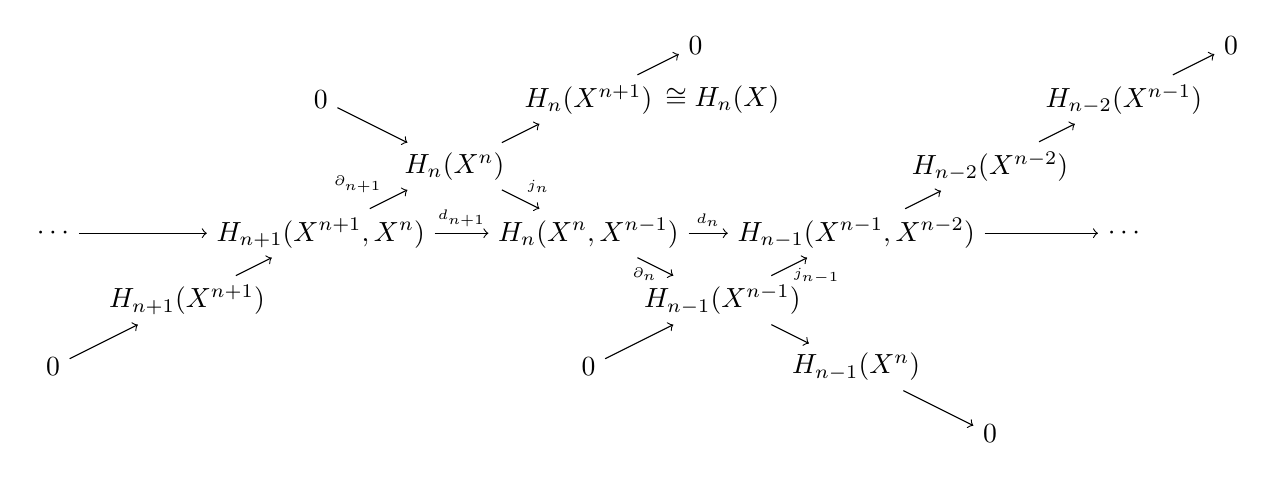
\begin{tikzpicture}[scale=0.85]
\node (0) at (0,0) {$\cdots$};
\node (k0) at (4,0) {$H_{n+1}(X^{n+1},X^n)$};
\node (k1) at (8,0) {$H_{n}(X^{n},X^{n-1})$};
\node (k2) at (12,0) {$H_{n-1}(X^{n-1},X^{n-2})$};
\node (k3) at (16,0) {$\cdots$};
\node (a1) at (6,1) {$H_n(X^n)$};
\node (a2) at (8,2) {$H_n(X^{n+1})$};
\node (s) at (10,2) {$\cong H_n(X)$};
\node (a3) at (9.6,2.8) {$0$};
\node (a4) at (4,2) {$0$};
\node (a5) at (14,1) {$H_{n-2}(X^{n-2})$};
\node (a6) at (16,2) {$H_{n-2}(X^{n-1})$};
\node (a7) at (17.6,2.8) {$0$};
\node (b1) at (10,-1) {$H_{n-1}(X^{n-1})$};
\node (b0) at (8,-2) {$0$};
\node (b2) at (2,-1) {$H_{n+1}(X^{n+1})$};
\node (b3) at (12,-2) {$H_{n-1}(X^n)$};
\node (b4) at (14,-3) {$0$};
\node (b5) at (0,-2) {$0$};
\draw[->]
(0) edge (k0)
(k0) edge node[node font=\tiny,auto] {$d_{n+1}$} (k1)
(k1) edge node[node font=\tiny,auto] {$d_{n}$} (k2)
(k2) edge (k3)
(k0) edge node[node font=\tiny,auto] {$\partial_{n+1}$} (a1) 
(a1) edge (a2)
(a2) edge (a3)
(a4) edge (a1)
(a1) edge node[node font=\tiny,auto] {$j_{n}$} (k1)
(k1) edge node[node font=\tiny,below,pos=0.2] {$\partial_{n}$} (b1) 
(b0) edge (b1)
(b1) edge node[node font=\tiny,below,pos=0.8,xshift=6pt] {$j_{n-1}$}(k2)
(b5) edge (b2)
(b2) edge (k0)
(b1) edge (b3)
(b3) edge (b4)
(k2) edge (a5)
(a5) edge (a6)
(a6) edge (a7);
\end{tikzpicture}\]
where $d_{n+1}$ and $d_n$ are defined as the compositions $j_n\partial_{n+1}$ and $j_{n-1}\partial_n$, which are just relativizations of the boundary maps $\partial_{n+1}$ and $\partial_n$. The composition $d_nd_{n+1}$ includes two successive maps in one of the exact sequences, hence is zero. Thus the horizontal row in the diagram is a chain complex, called the \textbf{cellular chain complex} of $X$ since $H_n(X_n,X_{n-1})$ is free with basis in one-to-one correspondence with the $n$ cells of $X$, so one can think of elements of $H_n(X_n,X_{n-1})$ as linear combinations of $n$ cells of $X$. The homology groups of this cellular chain complex are called the \textbf{cellular homology groups} of $X$. Temporarily we denote them $H^{CW}_n(X)$.
\begin{theorem}
$H^{CW}_n(X)=H_n(X)$.
\end{theorem}
\begin{proof}
From the diagram above, $H_n(X)$ can be identified with $H_n(X^n)/\im\partial_{n+1}$. Since $j_n$ is injective, it maps $\im\partial_{n+1}$ isomorphically onto $\im(j_n\partial_{n+1})=\im d_{n+1}$ and $H_n(X^n)$ isomorphically onto $\im j_n=\ker\partial_n$. Since $j_{n-1}$ is injective, $\ker\partial_n=\ker(j_{n-1}\partial_n)=\ker d_n$. Thus $j_n$ induces an isomorphism of the quotient $H_n(X^n)/\im\partial_{n+1}$ onto $\ker d_n/\im d_{n+1}$.
\end{proof}
Here are a few immediate applications:
\begin{itemize}
\item[$(\rmnum{1})$]$H_n(X)=0$ if $X$ is a CW complex with no $n$-cells.
\item[$(\rmnum{2})$]More generally, if $X$ is a CW complex with $k$ $n$-cells, then $H_n(X)$ is generated by at most $k$ elements. For since $H_n(X^n,X^{n-1})$ is free abelian on $k$ generators, the subgroup $\ker d_n$ must be generated by at most $k$ elements, hence also the quotient $\ker d_n/\im d_{n+1}$.
\item[$(\rmnum{3})$]If $X$ is a CW complex having no two of its cells in adjacent dimensions, then $H_n(X)$ is free abelian with basis in one-to-one correspondence with the $n$-cells of $X$. This is because the cellular boundary maps dn are automatically zero in this case.
\end{itemize}
An simple example is $S^n\times S^n$ with $n>1$, using the product CW structure consisting of a $0$-cell, two $n$-cells, and a $2n$-cell.\par
Next we describe how the cellular boundary maps dn can be computed. When
$n=1$ this is easy since the boundary map $d_1:H_1(X^1,X^0)\to H_0(X^0)$ is the same as the simplicial boundary map $\Delta_1(X)\to\Delta_0(X)$. In case $X$ is connected and has only one $0$-cell, then $d_1$ must be $0$, otherwise $H_0(X)$ would not be $\Z$. When $n>1$ we will show that $d_n$ can be computed in terms of degrees:
\begin{proposition}[\textbf{Cellular Boundary Formula}]
For an $n$-cell $e_\alpha^n$ in $X$, we have
\[d_n(e^n_\alpha)=\sum_\beta d_{\alpha\beta}e^{n-1}_\beta\]
where $d_{\alpha\beta}$ is the degree of the map 
\[S^{n-1}_\alpha\to X^{n-1}\to S^{n-1}_\beta\]
that is the composition of the attaching map of $e^n_\alpha$ with the quotient map collapsing $X^{n-1}-e^{n-1}_\beta$ to a point.
\end{proposition}
Here we are identifying the cells $e^n_\alpha$ and $e^{n-1}_\beta$ with generators of the corresponding summands of the cellular chain groups. The summation in the formula contains only finitely many terms since the attaching map of $e^n_\alpha$ has compact image, so this image
meets only finitely many cells $e^{n-1}_\beta$.
\begin{proof}
To derive the cellular boundary formula, consider the commutative diagram
\[\begin{tikzcd}
H_n(D_\alpha^n,\partial D_\alpha^n)\ar[d,"\Phi_{\alpha*}"]\ar[rr,"\partial","\cong"']&&\widetilde{H}_{n-1}(\partial D^n_\alpha)\ar[d,"\varphi_{\alpha*}"]\ar[rr,"\Delta_{\alpha\beta*}"]&&\widetilde{H}_{n-1}(S^{n-1}_\beta)\\
H_n(X^n,X^{n-1})\ar[rrd,swap,"d_n"]\ar[rr,"\partial_n"]&&\widetilde{H}_{n-1}(X^{n-1})\ar[d,"j_{n-1}"]\ar[rr,"q_*"]&&\widetilde{H}_{n-1}(X^{n-1}/X^{n-2})\ar[u,"q_{\beta*}"]\ar[d,"\cong"]\\
&&H_{n-1}(X^{n-1},X^{n-2})\ar[rr,"\cong"]&&H_{n-1}(X^{n-1}/X^{n-2},X^{n-2}/X^{n-2})
\end{tikzcd}\]
where
\begin{itemize}
\item $\Phi_\alpha$ is the characteristic map of the cell $e^n_\alpha$ and $\varphi_\alpha$ is its attaching map.
\item $q:X^{n-1}\to X^{n-1}/X^{n-2}$ is the quotient map.
\item $q_\beta:X^{n-1}/X^{n-2}\to S^{n-1}_\beta$ collapses the complement of the cell $e^{n-1}_\beta$ to a point, the resulting quotient sphere being identified with $S^{n-1}_\beta=D^{n-1}_\beta/\partial D^{n-1}_\beta$ via the characteristic map $\Phi_\beta$.
\item $\Delta_{\alpha\beta}:\partial D^n_\alpha\to S^{n-1}_\beta$ is the composition $q_\beta\circ q\circ\varphi_\alpha$, in other words, the attaching map of $e^n_\alpha$ followed by the quotient map $X^{n-1}\to S^{n-1}_\beta$ collapsing the complement of $e^{n-1}_\beta$ in $X^{n-1}$ to a point.
\end{itemize}
The map $\Phi_{\alpha*}$ takes a chosen generator $[D^n_\alpha]\in H_n(D^n_\alpha,\partial D^n_\alpha)$ to a generator of the $\Z$ summand of $H_n(X^n,X^{n-1})$ corresponding to $e^n_\alpha$. Letting $e^n_\alpha$ denote this generator, commutativity of the left half of the diagram then gives $d_n(e^n_\alpha)=j_{n-1}\circ\varphi_{\alpha*}\circ \partial[D^n_\alpha]$. In
terms of the basis for $H_{n-1}(X^{n-1},X^{n-2})$ corresponding to the cells $e^{n-1}_\beta$, the map $q_{\beta*}$ is the projection of $\widetilde{H}_{n-1}(X^{n-1},X^{n-2})$ onto its $\Z$ summand corresponding to $e^{n-1}_\beta$.cCommutativity of the diagram then yields the formula for $d_n$ given above.
\end{proof}
\begin{example}
Let $M_g$ be the closed orientable surface of genus $g$ with its usual CW
structure consisting of one $0$-cell, $2g$ $1$-cells, and one $2$-cell attached by the product of commutators $[a_1,b_1],\dots,[a_g,b_g]$. The associated cellular chain complex is
\[\begin{tikzcd}
0\ar[r]&\Z\ar[r,"d_2"]&\Z^{2g}\ar[r,"d_1"]&\Z\ar[r]&0
\end{tikzcd}\]
As observed above, $d_1$ must be $0$ since there is only one $0$-cell. Also, $d_2$ is $0$ because each $a_i$ or $b_i$ appears with its inverse in $[a_1,b_1]\cdots[a_g,b_g]$, so the maps $\Delta_{\alpha\beta}$ are
homotopic to constant maps. Since $d_1$ and $d_2$ are both zero, the homology groups of $M_g$ are the same as the cellular chain groups, namely, $\Z$ in dimensions $0$ and $2$, and $\Z^{2g}$ in dimension $1$.
\end{example}
\begin{example}
The closed nonorientable surface $N_g$ of genus $g$ has a cell structure
with one $0$-cell, $g$ $1$-cells, and one $2$-cell attached by the word $a^2_1a^2_2\cdots a^2_g$. Again $d_1=0$, and $d_2:\Z\to\Z^g$ is specified by the equation $d_2(1)=(2,\dots,2)$ since each $a_i$ appears in the attaching word of the $2$-cell with total exponent $2$, which means that
each $\Delta_{\alpha\beta}$ is homotopic to the map $z\mapsto z^2$, of degree $2$. Since $d_2(1)=(2,\dots,2)$, we have $d_2$ injective and hence $H_2(N_g)=0$. If we change the basis for $\Z^g$ by replacing
the last standard basis element $(0,\dots,1)$ by $(1,\dots,1)$, we see $H_1(N_g)=\Z^{g-1}\oplus\Z/2\Z$.
\end{example}
These two examples illustrate the general fact that the orientability of a closed connected manifold $M$ of dimension $n$ is detected by $H_n(M)$, which is $\Z$ if $M$ is orientable and $0$ otherwise.
\begin{example}[\textbf{An Acyclic Space}]
Let $X$ be obtained from $S^1\vee S^1$ by attaching two $2$-cells by the words $a^5b^{-3}$ and $b^3(ab)^{-2}$. Then $d_2:\Z^2\to\Z^2$ has matrix
\[\begin{pmatrix}
5&-2\\
-3&1
\end{pmatrix}\],
with the two columns coming from abelianizing $a^5b^{-3}$ and $b^3(ab)^{-2}$ to $5a-3b$ and $-2a+b$, in additive notation. The matrix has determinant $-1$, so $d_2$ is an isomorphism and $\widetilde{H}_i(X)=0$ for all $i$. Such a space $X$ is called \textbf{acyclic}.\par
We can see that this acyclic space is not contractible by considering $\pi_1(X)$, which has the presentation $\langle a,b\mid a^5b^{-3},b^3(ab)^{-2}\rangle$. There is a nontrivial homomorphism from this group to the group $G$ of rotational symmetries of a regular dodecahedron, sending $a$ to the rotation $\rho_a$ through angle $2\pi/5$ about the axis through the center of a pentagonal face, and $b$ to the rotation $\rho_b$ through angle $2\pi/3$ about the axis through a vertex of this face. The composition $\rho_a\rho_b$ is a rotation through angle $\pi$
about the axis through themidpoint of an edge abutting this vertex. Thus the relations $a^5=b^3=(ab)^2$ defining $\pi_1(X)$ become $\rho_a^5=\rho_b^3=(\rho_a\rho_b)^2=1$ in $G$, which means there is a well-defined homomorphism $\rho:\pi_1(X)\to G$ sending $a$ to $\rho_a$ and $b$ to $\rho_b$. It is not hard to see that $G$ is generated by $\rho_a$ and $\rho_b$, so $\rho$ is surjective. With more work one can compute that the kernel of $\rho$ is $\Z/2\Z$, generated by the element $a^5=b^3=(ab)^2$, and this $\Z/2\Z$ is in fact the center of $\pi_1(X)$. In particular, $\pi_1(X)$ has order $120$ since $G$ has order $60$.
\end{example}
Many more examples of a similar nature, quotients of a cube or other polyhedron with faces identified in some pattern, could be worked out in similar fashion. But let us instead turn to some higher-dimensional examples.
\begin{example}[\textbf{Moore Spaces}]
Given an abelian group $G$ and an integer $n\geq1$, we will construct a CW complex $X$ such that $H_n(X)=G$ and $\widetilde{H}_i(X)=0$ for $i\neq n$. Such a space is called a \textbf{Moore space}, commonly written $M(G,n)$ to indicate the dependence on $G$ and $n$. It is probably best for the definition of a Moore space to include the condition that $M(G,n)$ be simply-connected if $n>1$. The spaces we construct will have this property.\par
As an easy special case, when $G=\Z/m\Z$ we can take $X$ to be $S^n$ with a cell $e^{n+1}$ attached by a map $S^n\to S^n$ of degree $m$. More generally, any finitely generated $G$ can be realized by taking wedge sums of examples of this type for finite cyclic summands of $G$, together with copies of $S^n$ for infinite cyclic summands of $G$.\par
In the general nonfinitely generated case let $F\to G$ be a homomorphism of a free abelian group $F$ onto $G$, sending a basis for $F$ onto some set of generators of $G$. The kernel $K$ of this homomorphism is a subgroup of a free abelian group, hence is itself free abelian. Choose bases $\{x_\alpha\}$ for $F$ and $\{y_\beta\}$ for $K$, and write $y_\beta=\sum_\alpha d_{\beta\alpha}x_\alpha$. Let $X^n=\bigvee_\alpha S^n_\alpha$, so $H_n(X^n)=F$ via Corollary~\ref{homology wedge sum}. We will construct $X$ from $X^n$ by attaching cells $e^{n+1}_\beta$ via maps $f_\beta:S^n\to X^n$ such that the composition of $f_\beta$ with the
projection onto the summand $S^n_\alpha$ has degree $d_{\beta\alpha}$. Then the cellular boundary map $d_{n+1}$ will be the inclusion $K\hookrightarrow F$, hence $X$ will have the desired homology groups.\par
The construction of $f_\beta$ generalizes the construction in Example~\ref{map any degree} of a map $S^n\to S^n$ of given degree. Namely, we can let $f_\beta$ map the complement of $\sum_\alpha|d_{\beta\alpha}|$ disjoint balls in $S^n$ to the $0$ cell of $X^n$ while sending $|d_{\beta\alpha}|$ of the balls onto the summand $S^n_\alpha$ by maps of degree $+1$ if $d_{\beta\alpha}>0$, or degree $-1$ if $d_{\beta\alpha}<0$.
\end{example}
\begin{example}
By taking a wedge sum of the Moore spaces constructed in the preceding
example for varying $n$ we obtain a connected CW complex with any prescribed
sequence of homology groups in dimensions $1,2,3,\cdots$.
\end{example}
\begin{example}
As we have mensioned, $\RP^n$ has a CW structure with one cell $e^k$ in each dimension $k\leq n$, and the attaching map for $e^k$ is the $2$ sheeted covering projection $\varphi:S^{k-1}\to\RP^{k-1}$. To compute the boundary map $d_k$ we compute the degree of the composition 
\[\begin{tikzcd}
S^{k-1}\ar[r,"\varphi"]&\RP^{k-1}\ar[r,"q"]&\RP^{k-1}/\RP^{k-2}=S^{k-1}
\end{tikzcd}\]
with $q$ the quotient map. The map $q\varphi$ restricts to a homeomorphism from each component of $S^{k-1}-S^{k-2}$ onto $\RP^{k-1}-\RP^{k-2}$, and these two homeomorphisms are obtained from each other by precomposing with the antipodal map of $S^{k-1}$, which has degree $(-1)^k$. Hence $\deg q\varphi=\deg id+\deg(-id)=1+(-1)^k$, and so $d_k$ is either $0$ or multiplication by $2$ according to whether $k$ is odd or even. Thus the cellular chain complex for $\RP^n$ is
\[\begin{tikzcd}
0\ar[r]&\Z\ar[r,"2"]&\Z\ar[r,"0"]&\cdots\ar[r,"2"]&\Z\ar[r,"0"]&\Z\ar[r]&0
\end{tikzcd}\quad\text{if $n$ is even}\]
\[\begin{tikzcd}
0\ar[r]&\Z\ar[r,"0"]&\Z\ar[r,"2"]&\cdots\ar[r,"2"]&\Z\ar[r,"0"]&\Z\ar[r]&0
\end{tikzcd}\quad\text{if $n$ is odd}\]
From this it follows that
\[H_k(\RP^n)=\begin{cases}
\Z&\text{for $k=0$ and for $k=n$ odd}\\
\Z/2\Z&\text{for $k$ odd, $0<k<n$}\\
0&\text{otherwise}
\end{cases}\]
\end{example}
\begin{example}[\textbf{Lens Spaces}]
This example is somewhat more complicated. Given an integer $m>1$ and integers $\ell_1,\dots,\ell_n$ relatively prime to $m$, define the \textbf{lens space} $L=L_m(\ell_1,\dots,\ell_n)$ to be the orbit space $S^{2n-1}/(\Z/m\Z)$ of the unit sphere $S^{2n-1}\sub\C^n$ with the action of $\Z/m\Z$ generated by the rotation 
\[\rho(z_1,\dots,z_n)=(e^{2\pi i\ell_1/m}z_1,\dots,e^{2\pi i\ell_n/m}z_n),\]
rotating the $j$-th $\C$ factor of $\C^n$ by the angle $2\pi i\ell_j/m$ $($Note that by this definition, we can assume that $0<\ell_j<m$$)$. In particular, in the case $m=2$, $\ell_j$ can only be $1$, so $\rho$ is the antipodal map, so $L=\RP^{2n-1}$ in this case. In the general case, the projection $S^{2n-1}\to L$ is a covering space since the action of $\Z/m\Z$ on $S^{2n-1}$ is free: Only the identity element fixes any point of $S^{2n-1}$ since each point of $S^{2n-1}$ has some coordinate $z_j$
nonzero and then $e^{2\pi ik\ell_j/m}z_j\neq z_j$ for $0<k<m$, as a result of the assumption that $\ell_j$ is relatively prime to $m$.\par
We shall construct a CW structure on $L$ with one cell $e^k$ for each $k\leq 2n-1$ and show that the resulting cellular chain complex is
\[\begin{tikzcd}
0\ar[r]&\Z\ar[r,"0"]&\Z\ar[r,"m"]&\Z\ar[r,"0"]&\cdots\ar[r,"0"]&\Z\ar[r,"m"]&\Z\ar[r,"0"]&\Z\ar[r]&0
\end{tikzcd}\]
with boundary maps alternately $0$ and multiplication by $m$. Hence
\[H_k(L)=\begin{cases}
\Z&\text{for $k=0$ and for $k=2n-1$}\\
\Z/m\Z&\text{for $k$ odd, $0<k<2n-1$}\\
0&\text{otherwise}
\end{cases}\]
To obtain the CW structure, first subdivide the unit circle $C$ in the $n$-th $\C$ factor of $\C^n$ by taking the points $e^{2\pi ij/m}\in C$ as vertices, $j=1,\dots,m$. Joining the $j$-th vertex of $C$ to the unit sphere $S^{2n-3}\sub\C^{n-1}$ along arcs of great circles in $S^{2n-1}$ yields a $(2n-2)$-dimensional ball $B^{2n-2}_j$ bounded by $S^{2n-3}$ $(\partial B^{2n-2}=S^{2n-3})$. Specifically, $B^{2n-2}_j$ consists of the points \[\cos\theta(0,\dots,0,e^{2\pi ij/m})+\sin\theta(z_1,\dots,z_{n-1},0)\] for $0\leq\theta\leq\pi/2$, as $(z_1,\dots,z_{n-1})$ varies in $S^{2n-3}$. Similarly, joining the $j$-th edge of $C$ to $S^{2n-3}$ gives a ball $B^{2n-1}_j$ bounded by $B^{2n-2}_j$ and $B^{2n-2}_{j+1}$, subscripts being taken mod $m$ $(B^{2n-2}\times I\approx B^{2n-1})$. The rotation $\rho$ carries $S^{2n-3}$ to itself and rotates $C$ by the angle $2\pi\ell_n/m$, hence $\rho$ permutes the $B^{2n-2}_j$'s and the $B^{2n-1}_j$'s. A suitable power of $\rho$, namely ρr where $r\ell_n\equiv 1$ mod $m$, takes each $B^{2n-2}_j$ and $B^{2n-1}_j$ to the next one. Since $\rho^r$ has order $m$, it is also a generator of the rotation group $\Z/m\Z$, and hence we may obtain $L$ as the quotient of one $B^{2n-1}_j$ by identifying its two faces $B^{2n-2}_j$ and $B^{2n-2}_{j+1}$ together via $\rho^r$.\par
In particular, when $n=2$, $B^{2n-1}_j$ is a lens-shaped $3$ ball and $L$ is obtained from this ball by identifying its two curved disk faces via $\rho^r$, which may be described as the composition of the reflection across the plane containing the rim of the lens, taking one face of the lens to the other, followed by a rotation of this face through the angle $2\pi\ell/m$ where $\ell=r\ell_1$.\par
Returning to the construction of a CW structure on $L_m(\ell_1,\dots,\ell_n)$, observe that the $(2n-3)$-dimensional lens space $L_m(\ell_1,\dots,\ell_{n-1})$ sits in $L_m(\ell_1,\dots,\ell_n)$ as the quotient of $S^{2n-3}$, and $L_m(\ell_1,\dots,\ell_n)$ is obtained from this subspace by attaching two cells, of dimensions $2n-2$ and $2n-1$, coming from the interiors of $B^{2n-1}_j$ and its two identified faces $B^{2n-2}_j$ and $B^{2n-2}_{j+1}$. Inductively this gives a CW structure on
$L_m(\ell_1,\dots,\ell_n)$ with one cell $e^k$ in each dimension $k\leq2n-1$.\par
The boundary maps in the associated cellular chain complex are computed as
follows. The first one, $d_{2n-1}$, is zero since the identification of the two faces of $B^{2n-1}_j$ is via a reflection $($degree $-1$$)$ across $B^{2n-1}_j$ fixing $S^{2n-3}$, followed by a rotation $($degree $1$$)$, so $d_{2n-1}(e^{2n-1})=e^{2n-2}-e^{2n-2}$. The next boundary map $d_{2n-2}$ takes $e^{2n-2}$ to $me^{2n-3}$ since the attaching map for $e^{2n-2}$ is the quotient map $S^{2n-3}7\to L_m(\ell_1,\dots,\ell_{n-1})$ and the balls $B^{2n-3}_j$ in $S^{2n-3}$ which project down onto $e^{2n-3}$ are permuted cyclically by the rotation $\rho$ of degree $+1$. Inductively, the subsequent boundary maps $d_k$ then alternate between $0$ and multiplication by $m$.
\end{example}
\subsection{Topological Invariance of the Euler Characteristic}
Recall that the Euler characteristic of a finite CW complex $X$ is defined as
\[\chi(X)=\sum_{p=0}^{n}(-1)^pn_p.\]
where $n_p$ is the number of $p$-cells in $X$.
\begin{theorem}\label{Eular char}
If $X$ is a finite CW complex
\begin{align}\label{Eular char CW}
\chi(X)=\sum_{p}(-1)^p\rank H_p(X).
\end{align}
Therefore, the Euler characteristic is a homotopy invariant.
\end{theorem}
\begin{proof}
First let us assume that $X$ is connected.We prove $(\ref{Eular char CW})$ by induction on the number of cells of dimension $2$ or more. If $X$ has no such cells, then it is a connected graph. Exercise~\ref{Eular char graph} shows that $\pi_1(X)$ is a free group on $1-\chi(X)$ generators, and since for any set $S$, the abelianization of the free group $F(S)$ is isomorphic to the free abelian group $\Z^{\oplus S}$, $H_1(X)$ has rank $1-\chi(x)$. On the other hand, $H_0(X)$ has rank $1$ because $X$ is connected, and $H_p(X)=0$ for all other values of $p$, so $(\ref{Eular char CW})$ follows.\par
Now assume by induction that we have proved $(\ref{Eular char CW})$ for every finite CW complex with fewer than $k$ cells of dimension $2$ or more, and suppose $X$ has $k$ such cells. Let $e$ be any cell of maximum dimension $n$, and let $Z=X\setminus e$. It suffices to show that 
\[\chi(X)=\chi(Z)+(-1)^n\]
Let $\varphi:\partial D\to Z$ be the attaching map for $e$, and let $K$ and $L$ be the kernel and image of $\varphi_*:H_{n-1}(\partial D)\to H_{n-1}(Z)$, respectively. Then from Proposition~\ref{homology attach}, we have isomorphisms
\[H_p(Z)\cong H_p(X)\quad (p\neq n,n-1),\]
and exact sequences
\[\begin{tikzcd}
0\ar[r]&L\ar[r]&H_{n-1}(Z)\ar[r]&H_{n-1}(X)\ar[r]&0
\end{tikzcd}\]
\[\begin{tikzcd}
0\ar[r]&H_n(Z)\ar[r]&H_n(X)\ar[r]&K\ar[r]&0
\end{tikzcd}\]
It follows that
\[\rank H_p(X)=\rank H_p(Z)\quad(p\neq n,n-1).\]
\[\rank H_{n-1}(X)=\rank H_{n-1}(Z)-\rank L.\]
\[\rank H_n(X)=\rank H_n(Z)+\rank K.\]
Summing these equations with appropriate signs, and using the fact that \[\rank K+\rank L=\rank H_{n-1}(\partial D)=1,\] 
we obtain $(\ref{Eular char CW})$.\par
Finally, if $X$ is not connected, we can apply the preceding argument to each component of $X$, and then each side of $(\ref{Eular char CW})$ is the sum of the corresponding terms for the individual components.
\end{proof}
Motivated by this result, we make the following definitions. For any topological space $X$, the integer $\beta_p(X)=\rank H_p(X)$ (if it is finite) is called the $p$-th Betti number of $X$. We define the Euler characteristic of $X$ by
\[\chi(X)=\sum_p(-1)^p\beta_p(X).\]
provided that each $\beta_p(X)$ is finite and $\beta_p(X)=0$ for $p$ sufficiently large. It is a homotopy invariant, and the preceding theorem says that it can be computed for finite CW complexes as the alternating sum of the numbers of cells.
\subsection{Homology with Coefficients}
There is an easy generalization of the homology theory we have considered so far that behaves in a very similar fashion and sometimes offers technical advantages.\par
The generalization consists of using chains of the form $\sum_in_i\sigma_i$ where each $\sigma_i$ is a singular $n$ simplex in $X$ as before, but now the coefficients $n_i$ are taken to lie in a fixed abelian group $G$ rather than $\Z$ (That is, tensoring these chain groups with $G$). Such $n$ chains form an abelian group $C_n(X;G)$, and there is the expected relative version $C_n(X,A;G)=C_n(X;G)/C_n(A;G)$. The old formula for the boundary maps $\partial$ can still be used for arbitrary $G$, namely
\[\partial(\sigma)=\sum_i(-1)^i\sigma_i[v_0,\dots,\widehat{v}_i,\dots,v_n].\]
Just as before, a calculation shows that $\partial^2=0$, so the groups $C_n(X;G)$ and $C_n(X,A;G)$ form chain complexes. The resulting homology groups $H_n(X;G)$ and $H_n(X,A;G)$ are called \textbf{homology groups with coefficients in $\bm{G}$}. Reduced groups $\widetilde{H}_n(X;G)$ are defined via the augmented chain complex 
\[\begin{tikzcd}
\cdots\ar[r]&C_0(X;G)\ar[r,"\eps"]&G\ar[r]&0
\end{tikzcd}\]
with $\eps$ again defined by summing coefficients.\par
The case $G=\Z/2\Z$ is particularly simple since one is just considering sums of singular simplices with coefficients $0$ or $1$, so by discarding terms with coefficient $0$ one can think of chains as just finite \textit{unions} of singular simplices. The boundary formulas also simplify since one no longer has to worry about signs. Since signs are an algebraic representation of orientation considerations, one can also ignore orientations. This means that homology with $\Z/2\Z$ coefficients is often the most natural tool in the absence of \textit{orientability}.\par
All the theory we developed for $\Z$ coefficients carries over directly to general coefficient groups $G$ with no change in the proofs. The same is true for Mayer-Vietoris sequences. Differences between $H_n(X;G)$ and $H_n(X)$ begin to appear only when one starts making calculations. When $X$ is a point, the method used to compute $H_n(X)$ shows that $H_n(X;G)$ is $G$ for $n=0$ and $0$ for $n>0$. From this it follows just as for $G=Z$ that $\widetilde{H}_k(S^n;G)$ is $G$ for $k=n$ and $0$ otherwise.\par
Cellular homology also generalizes to homology with coefficients, with the cellular chain group $H_n(X^n,X^{n-1})$ replaced by $H_n(X^n,X^{n-1};G)$, which is a direct sum of $G$'s, one for each $n$ cell. The proof that the cellular homology groups $H^{CW}_n(X)$ agree with singular homology $H_n(X)$ extends immediately to give $H^{CW}_n(X;G)=H_n(X;G)$. The cellular boundary maps are given by the same formula as for $\Z$ coefficients,
\[d_n(e^n_\alpha)=\sum_\beta d_{\alpha\beta}e^{n-1}_\beta.\]
The old proof applies, but the following result is needed to know that the coefficients $d_{\alpha\beta}$ are the same as before:
\begin{lemma}\label{degree with coefficient}
If $f:S^k\to S^k$ has degree $m$, then $f_*:H_k(S^k;G)\to H_k(S^k;G)$ is multiplication by $m$.
\end{lemma}
\begin{proof}
As a preliminary observation, note that a homomorphism $\varphi:G_1\to G_2$ induces maps $\varphi_\sharp:C_n(X,A;G_1\to C_n(X,A;G_2)$ commuting with boundary maps, so there are induced homomorphisms $\varphi_*:H_n(X,A;G_1)\to H_n(X,A;G_2)$. These have various naturality properties. For example, they give a commutative diagram mapping the long exact sequence of homology for the pair $(X,A)$ with $G_1$ coefficients to the corresponding sequence with $G_2$ coefficients. Also, the maps $\varphi_*$ commute with homomorphisms $f_*$ induced by maps $f:(X,A)\to (Y,B)$.\par
Now let $f:S^k\to S^k$ have degree $m$ and let $\varphi:\Z\to G$ take $1$ to a given element $g\in G$. Then we have a commutative diagram as at the right, where commutativity of the outer two squares comes from the inductive calculation of these homology groups, reducing to the case $k=0$ when the commutativity is obvious.
\[\begin{tikzcd}
\Z\ar[d,"\varphi"]\ar[r,equal]&\widetilde{H}_k(S^k,\Z)\ar[d,"\varphi_*"]\ar[r,"f_*"]&\widetilde{H}_k(S^k,\Z)\ar[r,equal]\ar[d,"\varphi_*"]&\Z\ar[d,"\varphi"]\\
G\ar[r,equal]&\widetilde{H}_k(S^k,G)\ar[r,"f_*"]&\widetilde{H}_k(S^k,G)\ar[r,equal]&G
\end{tikzcd}\]
Since the diagram commutes, the assumption that the map across the top takes
$1$ to $m$ implies that the map across the bottom takes $g$ to $mg$.
\end{proof}
\begin{example}
It is instructive to see what happens to the homology of $\RP^n$ when the coefficient group $G$ is chosen to be a field $F$. The cellular chain complex is
\[\begin{tikzcd}
\cdots\ar[r,"0"]&F\ar[r,"2"]&F\ar[r,"0"]&F\ar[r,"2"]&F\ar[r,"0"]&F\ar[r]&0
\end{tikzcd}\]
Hence if $F$ has characteristic $2$, for example if $F=\Z/2\Z$, then $H_k(\RP^n;F)=F$ for $0\leq k\leq n$, a more uniform answer than with $\Z$ coefficients. On the other hand, if $F$ has characteristic different from $2$ then the boundary maps $F\stackrel{2}{\to}F$ are isomorphisms, hence $H_k(\RP^n;F)$ is $F$ for $k=0$ and for $k=n$ odd, and is zero otherwise.
\end{example}
As another illustration, we will now give an example of a map $f:X\to Y$ with the property that the induced maps $f_*$ are trivial for homology with $\Z$ coefficients but not for homology with $\Z/m\Z$ coefficients for suitably chosen $m$. Thus homology with $\Z/m\Z$ coefficients tells us that $f$ is not homotopic to a constant map, which we would not know using only $\Z$ coefficients.
\begin{example}
Let $X$ be a Moore space $M(\Z/m\Z,n)$ obtained from $S^n$ by attaching a cell $e^{n+1}$ by a map of degree $m$. The quotient map $f:X\to X/S^n=S^{n+1}$ induces trivial homomorphisms on reduced homology with $\Z$ coefficients since the nonzero reduced homology groups of $X$ and $S^{n+1}$ occur in different dimensions. But with $\Z/m\Z$ coefficients the story is different, as we can see by considering the long exact sequence of the pair $(X,S^n)$, which contains the segment
\[\begin{tikzcd}
0=\widetilde{H}_{n+1}(S^n;\Z/m\Z)\ar[r]&\widetilde{H}_{n+1}(X;\Z/m\Z)\ar[r,"f_*"]&\widetilde{H}_{n+1}(X/S^n;\Z/m\Z)
\end{tikzcd}\]
Exactness says that $f_*$ is injective. Since the cellular boundary map $H_{n+1}(X^{n+1},X^n;\Z/m\Z)\to H_{n+1}(X^{n},X^{n-1};\Z/m\Z)$ is $\Z/m\Z\stackrel{m}{\to}\Z/m\Z$, we get $\widetilde{H}_{n+1}(X;\Z/m\Z)=\Z/m\Z$, so $f_*$ is not zero.
\end{example}
\subsection{Exercise}
\begin{exercise}
Let $X^1,\dots,X^k$ be spaces with nondegenerate base points. For every $p>0$, show that $H_p(X^1\vee \cdots\vee X^k)\cong H_p(X^1)\oplus\cdots H_p(X^k)$.
\end{exercise}
\begin{proof}
Prove it by induction. We only need to deal with the case $k=2$. For $\{X^1,X^2\}$ regarded as subsets of $X^1\vee X^2$, use the Mayer-Vietories sequence we get the result since $X^1\cap X^2$ is a single point, which has homology zero for $p>0$.
\end{proof}
\begin{exercise}
\mbox{}
\begin{itemize}
\item[$(a)$]Suppose $U$ is an open subset of $\R^n$, $n\geq 2$. For any point $x\in U$, show that $H_{n-1}(U\setminus\{x\})\neq 0$.
\item[$(b)$]Show that if $m>n$, then $\R^m$ is not homeomorphic to any open subset of $\R^n$.
\end{itemize}
\end{exercise}
\begin{exercise}
Let $n\geq1$. Show that if $f:S^n\to S^n$ is a continuous map that has a continuous extension to a map $F:\widebar{\B}^{n+1}\to S^n$, then $f$ has degree zero.
\end{exercise}
\begin{proof}
$\widebar{\B}^{n+1}$ is contractible, hence has homology zero. In particular, the induced map $F_*=0$.
\end{proof}
\begin{exercise}
Show that if $n$ is even, then $Z/2\Z$ is the only nontrivial group that can act freely on $S^n$ by homeomorphisms.
\end{exercise}
\begin{proof}
If $G$ acts on $S^n$ by homeomorphisms, the degree defines a homomorphism from $G$ to $\{\pm 1\}$: if $\varphi:S^n\to S^n$ is a homeomorphism, $\deg\varphi=\pm 1$ since $\varphi$ has an inverse. Since $\deg(fg)=(\deg f)(\deg g)$, it is a homomorphism. By Theorem~\ref{degree fix point}, since $(-1)^{n+1}=-1$, if $\deg g=1$, then it has a fix point. However, since $G$ acts freely, we get $g=1$. Then degree is an injective homomorphism from $G$ to $\Z/2\Z$. Since $G$ is not trivial, it can only be $\Z/2\Z$.
\end{proof}
\begin{exercise}
Show that the dimension of a finite-dimensional CW complex is a topological invariant, and that any triangulation of an $n$-manifold has dimension $n$.
\end{exercise}
\begin{proof}
The dimension of a CW complex is the maximal dimansion of the neighborhood of its points. The triangulation of an $n$-manifold has dimension $n$ neighborhoods, so has dimension $n$.
\end{proof}
\begin{exercise}
Given a map $f:S^{2n}\to S^{2n}$, show that there is some point $x\in S^{2n}$ with either $f(x)=x$ or $f(x)=-x$. Deduce that every map $\RP^{2n}\to\RP^{2n}$ has a fixed point. Construct maps $\RP^{2n-1}\to\RP^{2n-1}$ without fixed points from linear transformations $\R^{2n}\to\R^{2n}$ without eigenvectors.
\end{exercise}
\begin{proof}
By Exercise~\ref{S^n map homotopic}, if $f(x)\neq x$ and $f(x)\neq -x$, then $f(x)\simeq -x\simeq x$. But by Proposition~\ref{antiplde map homotopy}, this is a contradiction.\par
For $\RP^{2n-1}$, consider the standard skrew-symmetry matrix:
\[A=\begin{pmatrix}
0&1\\
-1&0
\end{pmatrix}\]
and define an automorphism $\R^{2n}$ to $\R^{2n}$ by the matrix representation
\[\begin{pmatrix}
A&&\\
&\ddots&\\
&&A\\
\end{pmatrix}\]
of order $2n$. This is easily to verified to have no point satisfying $Ax=x$ or $Ax=-x$ since $A$ does not attain an real eigenvector, except $0$. Then on the sphere $S^{2n-1}$ it satisfies the requirement.
\end{proof}
\begin{exercise}
Let $f:S^n\to S^n$ be a map of degree zero. Show that there exist points $x,y\in S^n$ with $f(x)=x$ and $f(y)=-y$. Use this to show that if $F$ is a continuous vector field defined on the unit ball $D^n$ in $\R^n$ such that $F(x)\neq0$ for all $x$, then there exists a point on $\partial D^n$ where $F$ points radially outward and another point on $\partial D^n$ where $F$ points radially inward.
\end{exercise}
\begin{proof}
$\deg id=1$, $\deg(-id)=(-1)^{n+1}$. By Exercise~\ref{S^n map homotopic}, $\deg f$ is not equal to either of them, so there is some points such that $f(y)=-y$, $f(x)=x$.\par
If $F$ is a nonvanishing vector field on $D^n$, then $F(x)/|F(x)|$ is a nonzero map from $D^n$ to $S^{n-1}$, hence null-homotopic. So its restriction on $S^{n-1}$ has degree zero. By what we have proved, there is some points satisfies the condition.
\end{proof}
\begin{exercise}
Construct a surjective map $S^n\to S^n$ of degree zero, for each $n\geq 1$.
\end{exercise}
\begin{proof}
Define a rotation along the last coordinate.
\end{proof}
\begin{exercise}
Show that any two reflections of $S^n$ across different $n$-dimensional hyperplanes are homotopic, in fact homotopic through reflections
\end{exercise}
\begin{proof}
Choosing an $n$-dimensional hyperplane is the same as choosing a unit vector on $S^n$. The formula of reflection is given by
\[x\mapsto x-2(v\,|\,x)v.\]
where $|v|=1$. So a homotopy is immediate.
\end{proof}
\begin{exercise}
Show that every map $S^n\to S^n$ can be homotoped to have a fixed point if $n>0$.
\end{exercise}
\begin{proof}
If $f:S^n\to S^n$ has no fixed points, then it is homotopic to the antipodal map. If $n$ is odd, there is a homotopy from it to the identity by Theorem~\ref{antiplde map homotopy}. If $n$ is even, this does not work, since the homotopy does not exist in this case. But, if we consider
\begin{align*}
\big(&(x_1,x_2,...,x_{2m+1}),t\big)\mapsto\\
&(x_1\cos t-x_2\sin t,x_2\cos t+x_1\sin t,\dots,x_{2m-1}\cos t-x_{2m}\sin t,x_{2m}\cos t+x_{2m-1}\sin t,-x_{2m+1}).
\end{align*}
When $t=\pi$, this is the antipldal map. When $t=0$, this is the map
\[g:(x_1,\dots,x_{2m+1})\mapsto(x_!,\dots,-x_{2m+1}).\]
The restriction of $g$ on the equator $\{x\in S^n:x_{n+1}=0\}$ is a well define map from $S^{n-1}$ to $S^{n-1}$. So it has a fixed point. This fixed point is also that of $g$.
\end{proof}
\begin{exercise}\label{matrix local homology}
For an invertible linear transformation $f:\R^n\to\R^n$ show that the induced map on $H_n(\R^n,\R^n-\{0\})=\widetilde{H}_{n-1}(\R^n-\{0\})=\Z$ is $\mathrm{id}$ or $-\mathrm{id}$ according to whether the determinant of $f$ is positive or negative.
\end{exercise}
\begin{proof}
$SL(n,\R)$ has two connected component. By asumption, there are invertible matrices $P$ and $Q$ of positive determinant such that $PAQ=I_n$ or $-I_n$, depending on $\det A$. This gives a homotopy.
\end{proof}
\begin{exercise}
A polynomial $f(z)$ with complex coefficients, viewed as a map $\C\to \C$, can always be extended to a continuous map of one-point compactifications $\widehat{f}:S^2\to S^2$. Show
that the degree of $\widehat{f}$ equals the degree of $f$ as a polynomial. Show also that the local degree of $\widehat{f}$ at a root of $f$ is the multiplicity of the root.
\end{exercise}
\begin{proof}
We have the homotopy $t^nf(x/t)$ from $x^n$ to $f(x)$. Let $\widetilde{f}$ be the restriction of $\widehat{f}$ on $S^1\sub S^2$. Then the following diagram commutes
\[\begin{tikzcd}
H_2(S^2)\ar[r,"\partial"]\ar[d,"\widehat{f}_*"]&H_1(S^1)\ar[d,"\widetilde{f}_*"]\\
H_2(S^2)\ar[r,"\partial"]&H_1(S^1)
\end{tikzcd}\]
Since the restriction $\widetilde{f}_*$ has degree $n$ by our homotopy, $\widetilde{f}$ also has degree $n$.\par
We can choose a ball at each root such that it contains no other roots, so the local homology is just the multiplicity. 
\end{proof}
\begin{exercise}
Compute the homology groups of the following $2$ complexes:
\begin{itemize}
\item[$(a)$]The quotient of $S^2$ obtained by identifying north and south poles to a point.
\item[$(b)$]$S^1\times(S^1\vee S^1)$.
\item[$(c)$]The space obtained from $D^2$ by first deleting the interiors of two disjoint subdisks in the interior of $D^2$ and then identifying all three resulting boundary circles together via homeomorphisms preserving clockwise orientations of these circles.
\item[$(d)$]The quotient space of $S^1\times S^1$ obtained by identifying points in the circle $S^1\times\{x_0\}$ that differ by $2\pi/m$ rotation and identifying points in the circle $\{x_0\}\times S^1$ that differ by $2\pi/n$ rotation.
\end{itemize}
\end{exercise}
\begin{proof}
\mbox{}
\begin{itemize}
\item[$(a)$]Use the cell complex of one $0$-cell, two $1$-cells, one $2$-cells. Then we have a chain complex
\[\begin{tikzcd}
0\ar[r]&\Z\ar[r,"0"]&\Z^2\ar[r,"0"]&\Z\ar[r]&0
\end{tikzcd}\]
so $H_0(X)=H_2(X)=\Z$, $H_1(X)=\Z^2$.
\item[$(b)$]View it as two torus gluing along a big circle. The cell complex consists of one $o$-cell, three $1$-cells, two $2$-cells. The boundary map $\partial_1=\partial 2=0$, so $H_0(X)=\Z$, $H_0(X)=\Z^3$. $H_2(X)=\Z^2$.
\item[$(c)$]First we add two edges in the punctured disk. Labelling the edges, we get a cell complex with one $0$-cell, five $1$-cells, one $2$-cell. And the $2$-cell is attached by the edge labelling.
\begin{figure}[htpb]
\centering
\begin{minipage}{200pt}
\centering
\includegraphics[width=0.7\textwidth]{cell-1}
\caption{The cells.}
\end{minipage}
\hspace{20pt}
\begin{minipage}{200pt}
\centering
\includegraphics[width=0.8\textwidth]{cell-2}
\caption{Attaching presentation.}
\end{minipage}
\end{figure}
The boundary map is calculated as follows:
\[\left\{\begin{array}{l}
\partial_2(U)=a-d-a+d-e-a+e=-a,\\
\partial_1(a)=0, \partial_1(d)=0,\partial_1(e)=0\end{array}\right. \]
 we see that $\ker\partial_1=\Z^3$, $\im\partial_2=\Z$, $\ker\partial_2=0$. And we have the sequence
\[\begin{tikzcd}
0\ar[r]&\Z\ar[r,"\partial_2"]&\Z^3\ar[r,"\partial_1"]&\Z\ar[r]&0
\end{tikzcd}\]
It follows that $H_0(X)=\Z$, $H_1(X)=\Z^2$, $H_2(X)=0$.
\item[$(d)$]recall the chain complex of $T^2$:
\[\begin{tikzcd}
0\ar[r]&\Z\ar[r]&\Z^2\ar[r]&\Z\ar[r]&0
\end{tikzcd}\]$H_0(X)=\Z$ clearly, and $H_2(X)=0$ since $\partial_2$ is still injective. The identification does not change the cell structure and the boundary map, so the homology stays the same.
\end{itemize} 
\end{proof}
\begin{exercise}
Let $X$ be the quotient space of $S^2$ under the identifications $x\sim-x$ for $x$ in the equator $S^1$. Compute the homology groups $H_i(X)$. Do the same for $S^3$ with antipodal points of the equatorial $S^2\sub S^3$ identified.
\end{exercise}
\begin{proof}
This is the same as attaching two disks on $\RP^1$. So the homology is $H_0(X)=\Z$, $H_1(X)=\Z/2\Z$. But note that $\ker\partial_2$ is no longer zero, it is $U-V$, where $U,V$ are the $2$-cells. So $H_2(X)=\Z$.\par
Similar for the case $S^3$, we have $H_0(Y)=\Z$, $H_1(Y)=\Z/2\Z$, $H_2(Y)=0$, $H_3(Y)=\Z^2$.
\end{proof}
\begin{exercise}
Show that the quotient map $S^1\times S^1\to S^2$ collapsing the subspace $S^1\vee S^1$ to a point is not null-homotopic by showing that it induces an isomorphism on $H_2$. On the other hand, show via covering spaces that any map $S^2\to S^1\times S^1$ is null-homotopic.
\end{exercise}
\begin{proof}
$H_2(T)=H_2(S^2)=\Z$.
\end{proof}
\begin{exercise}
Let $X$ be the $2$ complex obtained from $S^1$ with its usual cell structure by attaching two $2$ cells by maps of degrees $2$ and $3$, respectively.
\begin{itemize}
\item[$(a)$]Compute the homology groups of all the subcomplexes $A\sub X$ and the corresponding quotient complexes $X/A$.
\item[$(b)$]Show that $X\simeq S^2$ and that the only subcomplex $A\sub X$ for which the quotient map $X\to X/A$ is a homotopy equivalence is the trivial subcomplex, the $0$ cell.
\end{itemize}
\end{exercise}
\begin{proof}
We do this by several steps. Denote the $2$-cells of $X$ by $U,V$, which have attaching map of degree $2$ and $3$, respectibely. Let $1$-cell be $a$.
\begin{itemize}
\item First, we compute the homology of $X$:
\[\begin{tikzcd}
0\ar[r]&\Z^2\ar[r,"\partial_2"]&\Z\ar[r,"\partial_1"]&\Z\ar[r]&0
\end{tikzcd}\]
Clearly $H_0(X)=0$. Since $X$ has only one $1$-cell, $\partial_1=0$. And
\[\partial_2(U)=2a,\quad \partial_2(V)=3a.\]
so $\ker\partial_2=3U-2V$, hence $H_2(X)=\Z$. Since $\im\partial_2=\Z$, we also get $H_1(X)=0$. Summerizing
\[\left\{\begin{array}{l}
H_2(X)=\Z\\
H_1(X)=0\\
H_0(X)=\Z
\end{array}\right. \]
\item Let us denote the subcomplex of $X$ by $X^2,X^3$ for the $1$-cells together with a single $2$-cell: $X^2=S^1\cup_2 U$, $X^3=S^1\cup_3 V$. Then
\[\left\{\begin{array}{l}
H_2(X^2)=0\\
H_1(X^2)=\Z/2\Z\\
H_0(X^2)=\Z
\end{array}\right. \quad
\left\{\begin{array}{l}
H_2(X^3)=0\\
H_1(X^3)=\Z/3\Z\\
H_0(X^3)=\Z
\end{array}\right. \]
\item The quotient complexes: $X/e^0=X$, $X/S^1=S^2\vee S^2$, $X/X^2=S^2$, $X/X^3=S^2$. The homology is well-known.
\item $X\to X/S^1$ is not a homotopy equivalence, since $H_2(S^2\vee S^2)=\Z^2$.\par
The quotient $q:X\to X/X^2$ is not a homotopy equivalence: $q_*$ maps the generator of $H_2(X)$, which is $-3U+2V$, to $2V$. Since $V$ is a generator of $X/X^2=S^2$, $q_*$ is not an isomorphism.\par
Similarly, $p:X\to X/X^3$ is not a homotopy equivalence.
\item $X\simeq S^2$: $\pi_1(X^2,e^0)=\Z/2\Z$, since $X^2=\RP^2$. The attaching map $3:S^1\to S^1\sub X^2$ is an element in $\pi_1(X^2,e^0)$, which is $[1]$ since $[3]=[1]$ in $\pi_1(X^2,e^0)$. Thus $3$ is homotopic to the degree one attaching map $1:S^1\to S^1\sub X^2$. Then
\begin{align*}
X&=X^2\cup_3 V\simeq X^2\cup_1 V=S^1\cup_2 U\cup_1 V=S^1\cup_1 V\cup_2 U\\
&=D^2\cup_2 U\simeq D^2\cup_0 U=D^2\vee S^2\simeq S^2
\end{align*}
\end{itemize}
\end{proof}
\begin{exercise}\label{even map even degree}
A map $f:S^n\to S^n$ satisfying $f(x)=f(-x)$ for all $x$ is called an \textbf{even map}. Show that an even map $S^n\to S^n$ must have even degree, and that the degree must in fact be zero when $n$ is even. When $n$ is odd, show there exist even maps of any given even degree.
\end{exercise}
\begin{proof}
Denote by $\alpha_n:S^n\to S^n$ the antipodal map. Then the map $f$ is even if
and only if
\[f\circ\alpha_n=f.\]
Hence 
\[\deg f=\deg(f\circ\alpha_n)=(-1)^{n+1}\deg f\]
Hence if $n$ is even then $\deg f=0$. Assume next that $n$ is odd.\par
Since $\RP^n=S^n/(x\sim-x)$ there exists a continuous map $g:\RP^n\to S^n$ such that the diagram below is commutative
\[\begin{tikzcd}
S^n\ar[r,"f"]\ar[dd,swap,"\pi"]&S^n\\
&\\
\RP^n\ar[ruu,swap,"g"]
\end{tikzcd}\]
Consider the collapse map $q:S^n\to\RP^{n}/\RP^{n-1}\approx S^n$. Arguing as in the proof of the Cellular Boundary Formula we deduce that the degree of the map
\[q\circ\pi:S^n\to \RP^n\to\RP^n/\RP^{n-1}\approx S^n\]
is $1+(-1)^{n+1}=2$. From the long exact sequence of the pair $(\RP^n,\RP^{n-1})$ we deduce that the natural map
\[\begin{tikzcd}
H_n(\RP^n)\ar[r,"j_n"]&H_n(\RP^n,\RP^{n-1})\cong H_n(\RP^n/\RP^{n-1})
\end{tikzcd}\]
is an isomorphism. By consulting the commutative diagram
\[\begin{tikzcd}
H_n(S^n)=\Z\ar[dd,"\pi_*"]\ar[rrdd,"(q\circ\pi)_*"]&&\\
&&\\
H_n(\RP^n)=\Z\ar[rr,"j_n"]&&H_n(\RP^n/\RP^{n-1})
\end{tikzcd}\]
we deduce that the induced $\pi_*$ is described by multiplication by $2$. Using this information we deduce that $\deg f=2\deg g$, so that $\deg f$ must be even.
\end{proof}
\begin{exercise}
Show that if $X$ is a CW complex then $H_n(X^n)$ is free by identifying it with the kernel of the cellular boundary map $H_n(X^n,X^{n-1})\to H_{n-1}(X^{n-1},X^{n-2})$.
\end{exercise}
\begin{proof}
Subgroup of a free group is free.
\end{proof}
\begin{exercise}
Let $\Delta^n=[v_0,\dots,v_n]$ have its natural $\Delta$-complex structure with $k$-simplices $[v_{i_0},\dots,v_{i_k}]$ for $i_0<\cdots<i_k$. Compute the ranks of the simplicial $($or cellular$)$ chain groups $\Delta_i(\Delta^n)$ and the subgroups of cycles and boundaries. Apply this to show that the $k$ skeleton of $\Delta^n$ has homology groups $\widetilde{H}_i((\Delta^n)^k)$ equal
to $0$ for $i<k$, and free of rank $\binom{n}{k+1}$ for $i=k$.
\end{exercise}
\begin{proof}
Clearly $\Delta^n$ has $\binom{n+1}{k+1}$ $k$-dimensional faces.\par
For $k=0$, the cycles has rank $n+1$, as the whole group. While boundary has rank $n$ since $H_0=\Z$. For $k=1$, the cycles and boundaries both have rank $\binom{n+1}{2}-n$ by the first isomorphism theorem and the fact that $H_1=0$. And for $k=2$, it becomes $\binom{n+1}{3}-\binom{n+1}{2}+n$ fro the same reason. Now concluding, in $\Delta_k$, the cycles and boundaries have rank
\[\binom{n+1}{k+1}-\binom{n+1}{k}+\cdots+(-1)^{k+1}\binom{n+1}{0}.\]
when $k=n$, this becomes $(1-1)^{n+1}$, so is zero.\par
Now we claim that 
\[\binom{n+1}{k+1}-\binom{n+1}{k}+\cdots+(-1)^{k+1}\binom{n+1}{0}=\binom{n}{k+1}\]
for $0\leq k<n$. In fact, from the formula 
\[\binom{n+1}{k+1}=\binom{n}{k+1}+\binom{n}{k}\]
we have the following
\begin{align*}
\sum_{i=0}^{k+1}(-1)^i\binom{n+1}{i}&=1+\sum_{i=1}^{k+1}(-1)^i\binom{n+1}{i}=\sum_{i=1}^{k+1}(-1)^i\Big[\binom{n}{i}+\binom{n}{i-1}\Big]\\
&=1+\sum_{i=1}^{k+1}(-1)^i\binom{n}{i}-\sum_{i=0}^{k}(-1)^i\binom{n}{i}\\
&=1+(-1)^{k+1}\binom{n}{k+1}-1=(-1)^{k+1}\binom{n}{k+1}.
\end{align*}
Now by changing the sign, we see our conclusion follows.\par
The rank of $\widetilde{H}_i((\Delta^n)^k)$ is that of cycles in $\Delta_k(\Delta^n)$.
\end{proof}
\begin{exercise}
Show the isomorphism between cellular and singular homology is natural in the following sense: A map $f:X\to Y$ that is \textbf{cellular}--satisfying $f(X^n)\sub Y^n$ for all $n$--induces a chain map $f_*$ between the cellular chain complexes of $X$ and $Y$, and the map $f_*:H^{CW}_n(X)\to H^{CW}_n(Y)$ induced by this chain map corresponds to $f_*:H_n(X)\to H_n(Y)$ under the isomorphism $H_n^{CW}=H_n$.
\end{exercise}
\begin{proof}
This comes from the naturality of the long exact sequence.
\end{proof}
\begin{exercise}
For a CW pair $(X,A)$ show there is a relative cellular chain complex formed by
the groups $H_i(X^i,X^{i-1}\cup A^i)$, having homology groups isomorphic to $H_n(X,A)$.
\end{exercise}
\begin{proof}
The idea is to quotient the $n$-cells in $X$ by $n$-cells in $A$. We have the following identification:
\[X^n/(X^{n-1}\cup A^n)\approx (X^n/A^n)/(X^{n-1}/A^{n-1}).\]
So consider the long exact sequence of the pair $(X^n/A^n,X^{n-1}/A^{n-1})$. And use $H_n(X^{n+1}/A^{n+1})=H_n(X/A)=H_n(X,A)$. We obtain the relative homology group.
\end{proof}
\begin{exercise}
Compute $H_i(\RP^n/\RP^m)$ for $m<n$ by cellular homology, using the standard CW
structure on $\RP^n$ with $\RP^m$ as its $m$ skeleton.
\end{exercise}
\begin{proof}
The CW complex consists of one $k$-cell, for $k=m+1,\dots,n$. The boundary map is the same.
\end{proof}

\begin{exercise}
If a finite CW complex X is the union of subcomplexes $A$ and $B$, show that
$\chi(X)=\chi(A)+\chi(B)-\chi(A\cap B)$.
\end{exercise}
\begin{proof}
For a finite CW complex $X$ let $c_n(X)$ denote the number of $n$-cells. Recall that the $n$-cells in $X\times Y$ are the products of an $i$-cell of $X$ and an $j$-cell of $Y$ with $i+j=n$, the claim is immediate.
\end{proof}
\begin{exercise}
For $X$ a finite CW complex and $p:\widetilde{X}\to X$ an $n$ sheeted covering space, show that $\chi(\widetilde{X})=n\chi(X)$.
\end{exercise}
\begin{exercise}
Show that if the closed orientable surface $M_g$ of genus $g$ is a covering space of $M_h$, then $g=n(h-1)+1$ for some $n$, namely, $n$ is the number of sheets in the covering.
\end{exercise}
\begin{proof}
$\chi(M_g)=2-2g$, $\chi(M_h)=2-2h$. Then
\[2-2g=n(2-2h)\Rightarrow g=n(h-1)+1\]
\end{proof}
\begin{exercise}
Show that for each $n\in\Z$ there is a unique function $\varphi$ assigning an integer to each finite CW complex, such that 
\begin{itemize}
\item[$(a)$]$\varphi(X)=\varphi(Y)$ if $X$ and $Y$ are homeomorphic.
\item[$(b)$]$\varphi(X)=\varphi(A)+\varphi(X/A)$ if $A$ is a subcomplex of $X$.
\item[$(c)$]$\varphi(S^0)=n$.
\end{itemize}
For such a function $\varphi$, show that $\varphi(X)=\varphi(Y)$ if $X\simeq Y$.
\end{exercise}
\begin{exercise}
Use the Mayer-Vietoris sequence to compute the homology groups of the space
obtained from a torus $S^1\times S^1$ by attaching a M\"obius band via a homeomorphismfrom the boundary circle of the M\"obius band to the circle $S^1\times\{x_0\}$ in the torus.\par
Do the same for the space obtained by attaching a M\"obius band to $\RP^2$ via a
homeomorphism of its boundary circle to the standard $\RP^1\sub\RP^2$.
\end{exercise}
\begin{exercise}
The surface $M_g$ of genus $g$, embedded in $\R^3$ in the standard way, bounds a
compact region $\R$. Two copies of $\R$, glued together by the identity map between their boundary surfaces $M_g$ , form a closed $3$-manifold $X$. Compute the homology groups of $X$ via the Mayer-Vietoris sequence for this decomposition of $X$ into two copies of $R$. Also compute the relative groups $H_i(R,M_g)$.
\end{exercise}
\begin{proof}
$R$ is the solid torus. The guled manifold is $S^3$, since it gives $\R^3/\partial\R^3$. The relative homology can be computed as
\[\left\{\begin{array}{l}
H_3(R,M_g)=\Z\\
H_2(R,M_g)=\Z\\
H_1(R,M_g)=0
\end{array}\right. \]
\end{proof}
\begin{exercise}
For the mapping torus $T_f$ of a map $f:X\to X$, we constructed in Example~\ref{two cylinder les} a long exact sequence
\[\begin{tikzcd}
\cdots\ar[r]&H_n(X)\ar[r,"\mathrm{id}-f_*"]&H_n(X)\ar[r]&H_n(T_f)\ar[r]&H_{n-1}(X)\ar[r]&\cdots
\end{tikzcd}\]
Use this to compute the homology of the mapping tori of the following maps:
\begin{itemize}
\item[$(a)$]A reflection $S^2\to S^2$.
\item[$(b)$]A map $S^2\to S^2$ of degree $2$.
\item[$(c)$]The map $S^1\times S^1\to S^1\times S^1$ that is the identity on one factor and a reflection on the other.
\item[$(d)$]The map $S^1\times S^1\to S^1\times S^1$ that is a reflection on each factor.
\item[$(e)$]The map $S^1\times S^1\to S^1\times S^1$ that interchanges the two factors and then reflects one of the factors.
\end{itemize}
\end{exercise}
\begin{proof}
\mbox{}
\begin{itemize}
\item[$(a)$]A reflection $S^2\to S^2$ has degree $-1$. So 
\[\begin{tikzcd}
0\ar[r]&H_3(T_f)\ar[r]&H_2(S^2)\ar[r,"2"]&H_2(S^2)\ar[r]&H_2(T_f)\ar[r]&0
\end{tikzcd}\]
Then $H_3(T_f)=0$, $H_2(T_f)=\Z/2\Z$ follows. We also have a short exact sequence
\[\begin{tikzcd}
0\ar[r]&H_1(T_f)\ar[r]&H_0(S^2)\ar[r,"0"]&H_0(S^2)\ar[r]&0
\end{tikzcd}\]
So $H_1(T_f)=\Z$. Clearly $H_0(T_f)=\Z$.
\[\left\{\begin{array}{l}
H_3(T_f)=0\\
H_2(T_f)=\Z/2\Z\\
H_1(T_f)=\Z\\
H_0(T_f)=\Z
\end{array}\right. \]
\item[$(b)$] Similarly, we get $H_3(T_f)=H_2(T_f)=0$, $H_1(T_f)=\Z$.
\[\left\{\begin{array}{l}
H_3(T_f)=0\\
H_2(T_f)=0\\
H_1(T_f)=\Z\\
H_0(T_f)=\Z
\end{array}\right. \]
\item The maps $f:S^1\to S^1$ are described by matrices $A:\Z^2\to \Z^2$. More precisely such a map defines a continuous map $\R^2\to\R^2$ which descends to quotients
\[A:\R^2/\Z^2\to\R^2/\Z^2.\]
Here are the matrices in the remaining three cases.
\[(c):\,\begin{pmatrix}
-1&0\\
0&1
\end{pmatrix}\quad(d):\,\begin{pmatrix}
-1&0\\
0&-1
\end{pmatrix}\quad(e):\,\begin{pmatrix}
-1&0\\
0&1
\end{pmatrix}\cdot\begin{pmatrix}
0&1\\
1&0
\end{pmatrix}=\begin{pmatrix}
0&-1\\
1&0
\end{pmatrix}\]
Suppose $f:S^1\times S^1\to S^1\times S^1$ is given by a $2\times2$ matrix $A$ with integral entries. We need to compute the induced maps $f_*:H_k(T^2)\to H_k(T^2)$. For $k=0$ we always have $f_*=\mathrm{id}$.\par
For $k=1$ we have $H_1(T^2)\cong H_1(S^1)\oplus H_1(S^1)=\Z^2$ and the induced map $f_*:\Z^2\to\Z^2$ coincides with the map induced by the matrix $A$.\par
For $k=2$ the induced map $f_*:\Z\to\Z$ can be identified with an integer, the degree of $f$. This integer is $\det A$, regardes as area change of the unit squre in $\R^2$. So we have
\[\begin{tikzcd}[row sep=tiny]
0\ar[r]&H_3(T_f)\ar[r]&H_2(T^2)\ar[r,"1-\det A"]&H_2(T^2)\ar[r]&H_2(T_f)\ar[r]&H_1(T^2)\ar[r,"1-A"]&{}\\
H_1(T^2)\ar[r]&H_1(T_f)\ar[r]&H_0(T^2)\ar[r,"0"]&H_0(T^2)\ar[r]&H_0(T_f)\ar[r]&0
\end{tikzcd}\]
\item In the case $(d)$ and $(e)$, since $\det A=1$ we have
\[H_3(T_f)=H_2(T^2)=\Z.\]
Consider the short exact sequences
\[\begin{tikzcd}
0\ar[r]&H_2(T^2)\ar[r]&H_2(T_f)\ar[r]&\ker(1-A)\ar[r]&0
\end{tikzcd}\]
In both cases $\ker(1-A)=0$ so that
\[H_2(T^2)=H_2(T_f)=\Z.\]
Finally we deduce a short exact sequence
\[\begin{tikzcd}
0\ar[r]&\coker(1-A)\ar[r]&H_1(T_f)\ar[r]&H_0(T^2)\ar[r]&0
\end{tikzcd}\]
so that
\[H_1(T_f)=\Z\oplus\coker(1-A).\]
In the case $(d)$ we have $1-A=\mathrm{id}$ so that $\coker=\Z/2\Z\oplus\Z/2\Z$.\par
In the case $(e)$ we have
\[1-A=\begin{pmatrix}
1&1\\
-1&1
\end{pmatrix}\longrightarrow\begin{pmatrix}
2&1\\
0&1
\end{pmatrix}\longrightarrow\begin{pmatrix}
2&0\\
0&1
\end{pmatrix}\]
The cokernel can be computed to be $\Z/2\Z$.
\[(d):\,\left\{\begin{array}{l}
H_3(T_f)=\Z\\
H_2(T_f)=\Z\\
H_1(T_f)=\Z\oplus\Z/2\Z\oplus\Z/2\Z\\
H_0(T_f)=\Z
\end{array}\right. \quad(e):\,\left\{\begin{array}{l}
H_3(T_f)=\Z\\
H_2(T_f)=\Z\\
H_1(T_f)=\Z\oplus\Z/2\Z\\
H_0(T_f)=\Z
\end{array}\right. \]
\item In the case $(c)$ we have $1-\det A=2$ and we have
\[H_3(T_f)=0.\]
Then we get an exact sequence
\[\begin{tikzcd}
0\ar[r]&\Z/2\Z\ar[r]&H_2(T_f)\ar[r]&\ker(1-A)\ar[r]&0
\end{tikzcd}\]
so $H_2(T_f)=\Z/2\Z\oplus\ker(1-A)$. Note that
\[1-A=\begin{pmatrix}
2&0\\
0&0
\end{pmatrix}\]
so $\ker(1-A)=\Z$, $H_2(T_f)=\Z\oplus\Z/2\Z$.\par
We get again 
\[H_1(T_f)=\Z\oplus\coker(1-A).\]
so $H_1(T_f)=\Z^2\oplus\Z/2\Z$.
\[(c):\,\left\{\begin{array}{l}
H_3(T_f)=0\\
H_2(T_f)=\Z\oplus\Z/2\Z\\
H_1(T_f)=\Z^2\oplus\Z/2\Z\\
H_0(T_f)=\Z
\end{array}\right. \]
\end{itemize}
\end{proof}
\begin{exercise}\label{homology prod with S^n}
Show that $H_i(X\times S^n)=H_i(X)\oplus H_{i-n}(X)$ for all $i$ and $n$, where $H_i=0$ for $i<0$ by definition. Namely, show 
\[H_i(X\times S^n)=H_i(X)\oplus H_i(X\times S^n,X\times\{x_0\}) \And H_i(X\times S^n,X\times\{x_0\})=H_{i-1}(X\times S^{n-1},X\times\{x_0\})\]
\end{exercise}
\begin{proof}
Let $x_1\in X,x_0\in S^n$. Define
\[A=X\times D^{n+1},\quad C=\{x_1\}\times\{x_0\}.\]
\[B=X\times S^n,\quad D=X\times\{x_0\}.\]
Then $A\cup B=X\times D^{n+1}$, $C\cup D=X\times\{x_0\}$. Since $D^{n+1}$ retracts to $\{x_0\}$, we have
\[H_i(A\cup B,C\cup D)=0.\]
So from the relative Mayer-Vietoris sequence,
\[H_i(A\cap B,C\cap D)=H_i(A,C)\oplus H_n(B,D).\]
That is,
\[H_i(X\times S^n)=H_i(X)\oplus H_i(X\times S^n,X\times\{x_0\}).\]
Now we prove $H_i(X\times S^n,X\times\{x_0\})=H_{i-1}(X\times S^{n-1},X\times\{x_0\})$: Write
\[S^n=D^n_+\cup D^n_-.\]
as the union of the upper and lower hemispheres. $S^{n-1}\sub S^n$ is their intersection, and choose $x_0\in S^{n-1}$. Note that
\[H_i(X\times D^n_-,X\times\{x_0\})=H_i(X\times D^n_+,X\times\{x_0\})=H_i(X\times\{x_0\},X\times\{x_0\})=0.\]
So the relative Mayer-Vietoris sequence gives
\[H_i(X\times S^n,X\times\{x_0\})=H_{i-1}(X\times S^{n-1},X\times\{x_0\}).\]
Now the result follows by ierating the identity:
\[H_i(X\times S^n,X\times\{x_0\})=H_{i-n}(X\times S^0,X\times \{x_0\})=H_{i-n}(X\times S^0/X\times\{x_0\})=H_{i-n}(X).\]
\end{proof}
\begin{exercise}
From the long exact sequence of homology groups associated to the short exact
sequence of chain complexes
\[\begin{tikzcd}
0\ar[r]&C_i(X)\ar[r,"\cdot n"]&C_i(X)\ar[r]&C_i(X;\Z/n\Z)\ar[r]&0
\end{tikzcd}\]
deduce immediately that there are short exact sequence
\[\begin{tikzcd}
0\ar[r]&H_i(X)/nH_i(X)\ar[r]&H_i(X;\Z/n\Z)\ar[r]&T_n(H_{i-1}(X))\ar[r]&0
\end{tikzcd}\]
where $T_n(G)$ denotes the $n$-torsion group of $G$, i.e., the kernel of the map
\[G\to G,\quad g\mapsto ng.\]
Use this to show that $\widetilde{H}_i(X;\Z/p\Z)=0$ for all $i$ and all primes $p$ iff $\widetilde{H}_i(X)$ is a vector space over $\Q$ for all $i$.
\end{exercise}
\begin{proof}
In the long exact sequence 
\[\begin{tikzcd}
\cdots\ar[r]&H_i(X)\ar[r,"\cdot n"]&H_i(X)\ar[r,"j"]&H_i(X,\Z/n\Z)\ar[r,"\partial"]&H_{i-1}(X)\ar[r,"\cdot n"]&H_{i-1}(X)\ar[r]&\cdots
\end{tikzcd}\]
We find that
\[\ker\partial=\im j=\coker(\cdot n)=H_i(X)/nH_i(X).\]
\[\im\partial=\ker(\cdot n)=T_n(H_{i-1}(X)).\]
So we get the short exact sequence.\par
If $\widetilde{H}_i(X;\Z/n\Z)=0$ for some $p$ and all $i$, then
\[H_i(X)/nH_i(X)=0,\quad T_n(H_{i-1}(X))=0.\]
The first shows that multiplication by $n$ is surjective, and the second means that it is injective. Now this holds for all prime $p$, so $1/p$ acts on $H_i(X)$ in the natural way. Since every integer $n$ can be written as
\[n=p_1^{r_1}\cdots p_n^{r_m}.\]
$1/n$ also acts on $H_i(X)$. Hence $\Q$ acts on $H_i(X)$, $H_i(X)$ is a $\Q$-vector space.\par
Now assume $H_i(X)$ is a $\Q$-vector space. Since $n\cdot(1/n\cdot\alpha)=\alpha$, we have $nH_i(X)=H_i(X)$ for all $n$ and all $i$. Further, if $n\alpha=0$, then $\alpha=1/n\cdot(n\alpha)=0$, which means $T_n(H_{i-1}(X))=0$ for all $n$ and all $i$. In particular, these hold for all prime $p$.
\end{proof}
\begin{exercise}
For $X$ a finite CW complex and $\F$ a field, show that the Euler characteristic $\chi(X)$ can also be computed by the formula \[\chi(X)=\sum_n(-1)^n\dim H_n(X;\F),\]
the alternating sum of the dimensions of the vector spaces $H_n(X;\F)$.
\end{exercise}
\begin{proof}
We have 
\[G\otimes\F=\F^r\]
where $r=\rank G$. This means tensoring with a field \textit{kills the torsion}.
\end{proof}
\begin{exercise}
Let $X$ be a finite connected graph having no vertex that is the endpoint of just one edge, and suppose that $H_1(X;\Z)$ is free abelian of rank $n>1$, so the group of automorphisms of $H_1(X;\Z)$ is $\GL_n(\Z)$, the group of invertible $n\times n$ matrices with integer entries whose inverse matrix also has integer entries. Show that if $G$ is a finite group of homeomorphisms of $X$, then the homomorphism $G\to\GL_n(\Z)$ assigning to $g:X\to X$ the induced homomorphism $g_*:H_1(X;\Z)\to H_1(X;\Z)$ is injective. Show the same result holds if the coefficient group $\Z$ is replaced by $\Z/m\Z$ with $m>2$. What goes wrong when $m=2$?
\end{exercise}
\begin{exercise}\label{homology structure}
\mbox{}
\begin{itemize}
\item[$(a)$]Show that a chain complex of \textbf{free abelian groups} $C_n$ splits as a direct sum of subcomplexes $0\to L_{n+1}\to K_n\to 0$ with at most two nonzero terms.
\item[$(b)$]In case the groups $C_n$ are finitely generated, show that $C_n$ splitting into summands $0\to\Z\to0$ and $0\to\Z\stackrel{m}{\longrightarrow}\Z\to0$.
\item[$(c)$]Deduce that if $X$ is a CW complex with finitely many cells in each dimension, then $H_n(X;G)$ is the direct sum of the following groups:
\begin{itemize}
\item a copy of $G$ for each $\Z$ summand of $H_n(X)$.
\item a copy of $G/mG$ for each $\Z/m\Z$ summand of $H_n(X)$.
\item a copy of the kernel of $G\stackrel{m}{\longrightarrow}G$ for each $\Z/m\Z$ summand of $H_{n-1}(X)$.
\end{itemize}
\end{itemize}
\end{exercise}
\begin{proof}
\mbox{}
\begin{itemize}
\item[$(a)$]The short exact sequence 
\[\begin{tikzcd}
0\ar[r]&\ker\partial_n\ar[r]&C_n\ar[r]&\im\partial_n\ar[r]&0
\end{tikzcd}\]
splits since $\im\partial$ is free. Hence there is a homomorphism $f_n:\im\partial_n\to C_n$ such that $\partial_n\circ f_n=\id$. The image of $f$ hence is free, and we have $C_n=\ker\partial_n\oplus\im f_n$ by splitness. Then we can write the complex as
\[\begin{tikzcd}
\vdots\ar[dd]&&\vdots\ar[dd]\\
&&\\
\ker\partial_n\ar[draw=none]{rr}[name=X, anchor=center,scale=1.5]{\oplus}\ar[dd,"0"]&&\im f_n\ar[lldd,"\partial_n"]\ar[dd,"0"]\\
&&\\
\ker\partial_{n-1}\ar[dd]\ar[draw=none]{rr}[name=X, anchor=center,scale=1.5]{\oplus}&&\im f_n\ar[dd]\\
&&\\
\vdots&&\vdots
\end{tikzcd}\]
So the complex can be decomposed into direct sums of the complexes
\[\begin{tikzcd}
0\ar[r]&\im f_n\ar[r,"\partial_n"]&\ker\partial_{n-1}\ar[r]&0
\end{tikzcd}\]
\item[$(b)$] If $C_n$ are finitely generated, we can use the elementary row and column operations to make $\partial_n:\im f_n\to\ker\partial_{n-1}$ into smith form. The smith form gives the decomposition $0\to\Z\to0$ and $0\to\Z\stackrel{m}{\longrightarrow}\Z\to0$.
\item[$(c)$] If we have a squence $0\to\Z\stackrel{m}{\longrightarrow}\Z\to0$, applying $\Hom(-,G)$ just gives $0\to G\stackrel{m}{\longrightarrow}G\to0$. Since by $(b)$, the homology $H_n(X)$ is just about the map $\partial_n:\im f_n\to\ker\partial_{n-1}$, which is a homomorphism between free abelian groups, so our claim comes from the following observations:
\begin{itemize}
\item First, each $\Z$ summand of $H_n(X)$ comes from the sequence $0\to\Z\to 0$, so this also gives a summand $G$ of $H_n(X;G)$.
\item Each $Z/m\Z$ summand of $H_n(X)$ comes from a sequence $0\to\Z\stackrel{m}{\longrightarrow}\Z\to0$ mapped from $C_{n+1}(X)$ to $C_n(X)$. So this will give a sequence $0\to G\stackrel{m}{\longrightarrow}G\to0$ mapped from $C_{n+1}(X;G)$ to $C_n(X;G)$, and yields a $G/mG$ summand on $H_n(X;G)$.
\item Similarly, each $\Z/m\Z$ summand of $H_{n-1}(X)$ comes from the same map $0\to\Z\stackrel{m}{\longrightarrow}\Z\to0$, but mapped from $C_{n}(X)$ to $C_{n+1}(X)$. In the case $\Z$ this makes no contribution to the kernel $\ker\partial_{n-1}$, but applying $\Hom(-,G)$ changes this, which adds a copy of the kernel $G\stackrel{m}{\longrightarrow}G$ to $\ker\partial_{n-1}$ now.
\end{itemize}
\end{itemize}
\end{proof}
\begin{exercise}[\textbf{Barratt-Whitehead Lemma}]\label{Barratt Whitehead lem}
Suppose we have the following commutative diagram of abelian groups, where the two rows are exact, and each morphism $\gamma_n:C_n\to F_n$ is an isomorphism:
\[\begin{tikzcd}
\cdots\ar[r]&C_{n+1}\ar[d,"\gamma_{n+1}","\sim"']\ar[r]&A_n\ar[d,"\alpha_n"]\ar[r]&B_n\ar[d,"\beta_n"]\ar[r]&C_n\ar[d,"\gamma_n","\sim"']\ar[r]&A_{n-1}\ar[d,"\alpha_{n-1}"]\ar[r]&\cdots\\
\cdots\ar[r]&F_{n+1}\ar[r]&D_n\ar[r]&E_n\ar[r]&F_n\ar[r]&D_{n-1}\ar[r]&\cdots
\end{tikzcd}\]
Show that this gives rise to an exact sequence
\[\begin{tikzcd}
\cdots\ar[r]&E_{n+1}\ar[r]&A_n\ar[r]&B_n\oplus D_n\ar[r]&E_n\ar[r]&A_{n-1}\ar[r]&\cdots
\end{tikzcd}\]
where the maps
are obtained from those in the previous diagram in the obvious way, except that
$B_n\oplus D_n\to E_n$ has a minus sign in one coordinate.
\end{exercise}
\begin{proof}
Relabelling the sequence such that we can write the morphisms in the induced sequence:
\[\begin{tikzcd}
\cdots\ar[r]&C_{n+1}\ar[d,"\gamma_{n+1}","\sim"']\ar[r,"k_{n+1}"]&A_n\ar[d,"\alpha_n"]\ar[r,"i_n"]&B_n\ar[d,"\beta_n"]\ar[r,"j_n"]&C_n\ar[d,"\gamma_n","\sim"']\ar[r,"k_n"]&A_{n-1}\ar[d,"\alpha_{n-1}"]\ar[r]&\cdots\\
\cdots\ar[r]&F_{n+1}\ar[r,"k'_{n+1}"]&D_n\ar[r,"i'_n"]&E_n\ar[r,"j'_n"]&F_n\ar[r,"k'_n"]&D_{n-1}\ar[r]&\cdots
\end{tikzcd}\]
Then the long exact sequence is
\[\begin{tikzcd}
\cdots\ar[r]&A_n\ar[rr,"{(i_n,\alpha_n)}"]&&B_n\oplus D_n\ar[rr,"\beta_n-i'_n"]&&E_n\ar[rr,"k_n\circ\gamma_n^{-1}\circ j'_n"]&&A_{n-1}\ar[r]&\cdots
\end{tikzcd}\]
This is a complex from the commutativity of the big diagram. Now we check the exactness.
\begin{itemize}
\item[$(a)$]Assume $(b,c)\in B_n\oplus D_n$ satisfies $\beta_n(b)-i'_n(d)=0$. Then $j'_n\circ \beta_n(b)=0$ since $j'_n\circ i'_n=0$. By the commutativity and $\gamma_n$ is injective, we get $j_n(b)=0$ and hence $b=i_n(a)$ for some $a\in A_n$. This also means
\[i'_n\circ\alpha_n(a)=\beta_n\circ i_n(a)=i'_n(d).\]
So we write $d=\alpha_n(a)+d'$ where $d'\in\ker i'_n$. Now by the exactness and that $\gamma_{n+1}$ is surjective, \[d'=k'_{n+1}(f)=k'_{n+1}\circ\gamma_{n+1}(c)\text{ for }c\in C_{n+1}.\]
Then We conclude
\[d=\alpha_n(a)+d'=\alpha_n(a)+k'_{n+1}\circ\gamma_{n+1}(c)=\alpha_n(a)+\alpha_n\circ k_{n+1}(c)=\alpha_n(a+k_{n+1}(c)).\]
Also note that
\[i_n(a+k_{n+1}(c))=i_n(a)=b\]
so $a+k_{n+1}(c)$ is what we need. This gives the exactness at $B_n\oplus D_n$.
\item Given $e\in E_n$ such that $k_n\circ\gamma_n^{-1}\circ j'_n(e)=$. First note that $\gamma_n^{-1}\circ j'_n(e)\in\ker k_n=\im j_n$, so $\gamma_n^{-1}\circ j'_n(e)=j_n(b)$. And
\[j'_n\circ\beta_n(b)=\gamma_n\circ j_n(b)=j'_n(e),\]
which gives $e=\beta_n(b)+e'$ for $e'\in\ker j'_n$. Again by exactness, $e'=i'_n(d)$ therefore
\[e=\beta_n(b)+i'_n(d)=(\beta_n-i'_n)(b,-d).\]
Hence our claim follows.
\item Finally, let $a\in A_{n-1}$ such that $(i_{n-1},\alpha_{n-1})(a)=0$. Then $i_{n-1}(a)=0$ and $\alpha_{n-1}(a)=0$. By exactness of first row, $a=k_n(c)$ for some $c\in C_n$. And 
\[k'_n\circ\gamma_n(c)=\alpha_{n-1}\circ k_n(c)=\alpha_{n-1}(a)=0.\]
so $\gamma_n(c)=j'_n(e)$ for some $e\in E_n$. Since $\gamma_n$ is an isomorphism ,this already gives 
\[k_n\circ\gamma_n^{-1}\circ j'_n(e)=a.\]
so we are done.
\end{itemize}
\end{proof}
\section{Additional topics}
\subsection{Eilenberg-Steenrod Axioms}
\begin{definition}
Let $\mathcal{C}$ and $\mathcal{D}$ be two categories, and let $F,G:\mathcal{C}\to\mathcal{D}$ be two functors. A \textbf{natural transformation} $\mu:F\to G$ is a family of morphisms $\mu_X:F(X)\to G(X)$ for each $X\in\mathrm{obj}(\mathcal{C})$ such that for any morphism $f:A\to B$ in $\mathcal{C}$ the following diagram commutes:
\[\begin{tikzcd}
F(A)\ar[d,swap,"F(f)"]\ar[r,"\mu_A"]&G(A)\ar[d,"G(f)"]\\
F(B)\ar[r,"\mu_A"]&G(B)
\end{tikzcd}\]
If each morphism $\mu_X$ is an isomorphism then we say that $\mu$ is a \textbf{natural isomorphism}.
\end{definition}
\begin{example}
\mbox{}
\begin{itemize}
\item[$(a)$]A finite-dimensional vector space is naturally isomorphic to its double dual.
\item[$(b)$]Regard $\pi_1$ and $H_1$ as functors $\mathsf{Top}_*\to\mathsf{Grp}$ $($i.e. forget that $H_1(X)$ is abelian$)$. Then the Hurewicz map denes a natural transformation $\pi_1\to H_1$.
\item[$(c)$]Let $\mathsf{Top}^2$ denote the pairs of topology spaces, that is, $\mathsf{Top}^2=\mathsf{Top}\times\mathsf{Top}$. Define a functor \[R:\mathsf{Top}^2\to\mathsf{Top}^2,\quad R(X,X')=(X',\emp).\]
Then the connecting homomorphism $\delta$ of the long exact sequence of a pair defines a natural transformation $\delta:H_n\to H_{n-1}\circ R$.
\end{itemize}
\end{example}
With the definition of natural transformations out of the way, we can finally introduce the famous \textit{Eilenberg-Steenrod axioms} for a homology theory. Let $R:\mathsf{Top}^2\to\mathsf{Top}^2$ be as in the previous example.
\begin{definition}[\textbf{The Eilenberg-Steenrod Axioms}]
A \textbf{homology theory} is a sequence $\mathscr{H}_n:\mathsf{Top}^2\to\mathsf{Ab}$ of functors for $n\geq0$ and a sequence $\delta=\delta_n:\mathscr{H}_n\to\mathscr{H}_{n-1}\circ R$ of natural transformations for $n\geq1$ satisfying the following four axioms:
\begin{itemize}
\item \textbf{The homotopy axiom}: If $f,g:(X,X')\to(Y,Y')$ are homotopic rel $X'$, then $\mathscr{H}_n(f)=\mathscr{H}_n(g)$ for all $n\geq0$. Thus $\mathscr{H}_n$ factors to define functors $\mathsf{hTop}^2\to\mathsf{Ab}$ for each $n\geq0$.
\item \textbf{The exact sequence axiom}: For every pair $(X,X')$ with inclusions $i:(X',\emp)\hookrightarrow(X,X')$ and $j:(X,\emp)\hookrightarrow(X,X')$, there is an exact sequence
\[\begin{tikzcd}
\cdots\ar[r]&\mathscr{H}_n(X')\ar[r,"\mathscr{H}_n(i)"]&\mathscr{H}_n(X)\ar[r,"\mathscr{H}_n(j)"]&\mathscr{H}_n(X,X')\ar[r,"\delta"]&\mathscr{H}_{n-1}(X')\ar[r]&\cdots
\end{tikzcd}\]
where we abbreviate $\mathscr{H}_n(X)=\mathscr{H}_n(X,\emp)$ etc.
\item \textbf{The excision axiom}: For every pair $(X,X')$ and every subset $U\sub X$ with $\widebar{U}\sub\Int(X')$, the inclusion $(X\setminus U,X'\setminus U)\hookrightarrow(X,X')$ induces an isomorphism
\[\mathscr{H}_n(X\setminus U,X'\setminus U)\cong\mathscr{H}_n(X,X').\]
\item \textbf{The dimension axiom}: If $\{\ast\}$ is a one-point space then $\mathscr{H}_n(\ast)=0$ for all $n>0$ and $\mathscr{H}_0(\ast)=\Z$.
\end{itemize}
There are additionally two optional axioms:
\begin{itemize}
\item \textbf{The additivity axiom}: Let $(X_\lambda,X_\lambda')$, $\lambda\in\Lambda$ be a family of pairs of spaces. Denote by
\[i_\lambda:(X_\lambda,X_\lambda')\hookrightarrow \Big(\coprod_\lambda X_\lambda,\coprod_\lambda X'_\lambda\Big)\]
inclusion. Then for all $n\geq0$, the map
\[\sum_\lambda\mathscr{H}_n(i_\lambda):\bigoplus_\lambda\mathscr{H}_n(X_\lambda,X'_\lambda)\to\mathscr{H}_n\Big(\coprod_\lambda X_\lambda,\coprod_\lambda X'_\lambda\Big)\]
is an isomorphism.
\item \textbf{The weak equivalence axiom}: If $f:(X,X')\to(Y,Y')$ is a weak equivalence then $\mathscr{H}_n(f):\mathscr{H}_n(X,X')\to\mathscr{H}_n(Y,Y')$ is an isomorphism for all $n\geq0$.
\end{itemize}
\end{definition}
We have seen how Mayer-Vietoris sequences can be quite useful for singular homology, and in fact every homology theory has Mayer-Vietoris sequences, at least for CW complexes. These can be obtained directly from the axioms in the following way. For a CW complex $X=A\cup B$ with $A$ and $B$ subcomplexes, the inclusion $(B,A\cap B)\hookrightarrow(X,A)$ induces a commutative diagram of exact sequences
\[\begin{tikzcd}
\cdots\ar[r]&\mathscr{H}_{n+1}(B,A\cap B)\ar[d,"\sim"]\ar[r]&\mathscr{H}_n(A\cap B)\ar[d]\ar[r]&\mathscr{H}_n(B)\ar[d]\ar[r]&\mathscr{H}_n(B,A\cap B)\ar[d,"\sim"]\ar[r]&\cdots\\
\cdots\ar[r]&\mathscr{H}_{n+1}(X,A)\ar[r]&\mathscr{H}_n(A)\ar[r]&\mathscr{H}_n(X)\ar[r]&\mathscr{H}_n(X,A)\ar[r]&\cdots
\end{tikzcd}\]
The vertical maps between relative groups are isomorphisms fro excision. Then it is a purely algebraic fact, the Barratt-Whitehead Lemma: a diagram such as this with every third vertical map an isomorphism gives rise to a long exact sequence involving the remaining nonisomorphic terms. In the present case this takes the form of a Mayer-Vietoris sequence
\[\begin{tikzcd}
\cdots\ar[r]&\mathscr{H}_{n+1}(X)\ar[r]&\mathscr{H}_n(A\cap B)\ar[r]&\mathscr{H}_n(A)\oplus\mathscr{H}_n(B)\ar[r]&\mathscr{H}_n(X)\ar[r]&\cdots
\end{tikzcd}\]
This can also be served as an alternative proof for the original Mayer-Vietoris sequence.
\subsection{Classical Applications}
In this section we use homology theory to prove several interesting results in
topology and algebra whose statements give no hint that algebraic topology might be involved.\par
To begin, we calculate the homology of complements of embedded spheres and
disks in a sphere. Recall that an embedding is a map that is a homeomorphism onto its image.
\begin{proposition}
\mbox{}
\begin{itemize}
\item[$(a)$] For an embedding $h:D^k\to S^n$, $\widetilde{H}_i(S^n-h(D^k))=0$ for all $i$.
\item[$(a)$] For an embedding $h:S^k\to S^n$ with $k<n$, $\widetilde{H}_i(S^n-h(S^k))$ is $\Z$ for $i=n-k-1$ and $0$ otherwise.
\end{itemize}
\end{proposition}
\begin{proof}
We prove $(a)$ by induction on $k$. When $k=0$, $S^n-h(D^0)$ is homeomorphic to $\R^n$, so this case is trivial.\par
For the induction step it will be convenient to replace the domain disk $D^k$ of $h$ by the cube $I^k$. Let $A=S^n-h(I^{k-1}\times[0,1/2])$ and $B=S^n-h(I^{k-1}\times[1/2,1])$, so 
\[A\cap B=S^n-h(I^k),\quad A\cup B=S^n-h(I^{k-1}\times\{1/2\})\]
By induction $\widetilde{H}_i(A\cup B)=0$ for all $i$, so the Mayer-Vietoris sequence gives isomorphisms \[\Phi:\widetilde{H}_i(S^n-h(I^k))\to\widetilde{H}_i(A)\oplus\widetilde{H}_i(B)\]
for all $i$. Modulo signs, the two components of $\Phi$ are induced by the inclusions $S^n-h(I^k)֓\hookrightarrow A$ and $S^n-h(I^k)֓\hookrightarrow B$, so if there exists an $i$-dimensional cycle $\alpha$ in $S^n-h(I^k)$ that is not a boundary in $S^n-h(I^k)$, then $\alpha$ is also not a boundary in at least one of $A$ and $B$. (When $i=0$ the word cycle here is to be interpreted in the sense of augmented chain complexes since we are dealing with reduced homology.) By iteration we can then produce a nested sequence of closed intervals \[I_1\sups I_2\sups\cdots\]
in the last coordinate of $I^k$ shrinking down to a point $p\in I$, such that $\alpha$ is not a boundary in $S^n-h(I^{k-1}\times I_m)$ for any $m$.\par
On the other hand, by induction on $k$ we know that $\alpha$ is the boundary of a chain $\beta$ in 
\[S^n-h(I^{k-1}\times\{p\})\approx S^n-h(D^{k-1})\]
since it has trivial homology. This $\beta$ is a finite linear combination of singular simplices with compact image in $S^n-h(I^{k-1}\times\{p\})$. The union of these images is covered by the nested sequence of open sets $\{S^n-h(I^{k-1}\times I_m)\}$, so by compactness $\beta$ must actually be a chain in $S^n-h(I^{k-1}\times I_m)$ for some $m$. This contradiction shows that $\alpha$ must be a boundary in $S^n-h(I^k)$, finishing the induction step.\par
Part $(b)$ is also proved by induction on $k$, starting with the trivial case $k=0$ when $S^n-h(S^0)$ is homeomorphic to $S^{n-1}\times\R$, so 
\[\widetilde{H}_i(S^n-h(S^0))=\widetilde{H}_i(S^{n-1}\times\R)=\widetilde{H}_i(S^{n-1})=\begin{cases}
\Z&i=n-1\\
0&\text{otherwise}
\end{cases}\]
For the induction step, write $S^k$ as the union of hemispheres $D^k_+$ and $D^k_−$ intersecting in $S^{k-1}$. Similar to the proof of $(a)$, let $A=S^{n}-h(D^k_+)$ and $B=S^n-h(D^k_-)$, then 
\[A\cap B=S^n-h(S^k),\quad A\cup B=S^n-h(S^{k-1}).\]
While $A$ and $B$ both have trivial reduced homology by part $(a)$. Then the Mayer-Vietories sequence gives isomorphisms \[\widetilde{H}_i(S^n-h(S^k))\approx\widetilde{H}_{i+1}(S^n-h(S^{k-1}))\]
And the claim follows by iterating:
\[\widetilde{H}_i(S^n-h(S^k))=\widetilde{H}_{i+k}(S^n-h(S^0))=\widetilde{H}_{i+k}(S^{n-1})=\begin{cases}
\Z&\text{if }i+k=n-1\\
0&\text{otherwise}
\end{cases}\]
\end{proof}
If we apply the last part of this proof to an embedding $h:S^n\to S^n$, the Mayer-Vietoris sequence ends with the terms \[\widetilde{H}_0(A)\oplus\widetilde{H}_0(B)\to\widetilde{H}_0(S^n-h(S^{n-1}))\to 0\]
Both $\widetilde{H}_0(A)$ and $\widetilde{H}_0(B)$ are zero, so exactness would imply that $\widetilde{H}_0(S^n-h(S^{n-1}))=0$, which appears to contradict the fact that $S^n-h(S^{n-1})$ has two path-components. The only way out of this dilemma is for $h$ to be surjective, so that $A\cap B$ is empty and the $0$ at the end of the Mayer-Vietoris sequence is $\widetilde{H}_{-1}(\emp)$ which is $\Z$ rather than $0$.\par
In particular, this shows that $S^n$ cannot be embedded in $\R^n$ since this would yield a nonsurjective embedding in $S^n$. A consequence is that there is no embedding $\R^m֓\hookrightarrow\R^n$ for $m>n$ since this would restrict to an embedding of $S^n\sub\R^m$ into $\R^n$. More generally there is no continuous injection $\R^m\to\R^n$ for $m>n$ since this too would give an embedding $S^n֓\hookrightarrow\R^n$.

\begin{example}[\textbf{The Alexander Horned Sphere}]
This is a subspace $S\sub\R^3$ homeomorphic to $S^2$ such that the unbounded component of $\R^3-S$ is not simply-connected as it is for the standard $S^2\sub\R^3$. We will construct $S$ by defining a sequence of compact subspaces $X_0\sups X_1\sups \cdots$ of $\R^3$ whose intersection is homeomorphic to a ball, and then $S$ will be the boundary sphere of this ball.\par
In the following by a handle we mean a \textbf{solid handle} $I\times D^2$. \textbf{Attaching a handle} means forming the connected sum along the boundary $\partial I\times D^2$. And the balls and handles are all defined to be  \textbf{closed subsets} of $\R^3$.
\begin{itemize}
\item We begin with $X_0$ a solid torus $S^1\times D^2$ obtained from a ball $B_0$ by attaching a handle.
\item To form the space $X_1\sub X_0$ we delete part of the short handle of $X_0$, from which we get two disks on the handles. Then we attach two smaller handles on the disks obtained from deleting, and we make these two handles cross. 
\item To form $X_2$ the process is repeated: Delete part of the handles attached on the last step, and attach smaller handles.
\item In the same way $X_n$ is constructed inductively from $X_{n-1}$. Thus $X_n$ is a ball $B_n$ with $2^n$ handles attached, and $B_n$ is obtained from $B_{n-1}$ by attaching $2^n$ horns.
\end{itemize}
There are homeomorphisms $h_n:B_{n-1}\to B_n$ that are the identity outside a small neighborhood of $B_n-B_{n-1}$. As $n$ goes to infinity, the composition $h_n\cdots h_1$ approaches a map $f:B_0\to\R^3$ which is continuous since the convergence is uniform. The set of points in $B_0$ where $f$ is not equal to $h_n\cdots h_1$ for large $n$ is a Cantor set, whose image under $f$ is the intersection of all the handles. It is not hard to see that $f$ is one-to-one. By compactness it follows that $f$ is a homeomorphism onto its image, a ball $B\sub\R^3$ whose boundary sphere $f(\partial B_0)$ is $S$, the Alexander horned sphere.\par
Now we compute $\pi_1(\R^3-B)$. Note that $B=\bigcap_nX_n$, so $\R^3-B=\bigcup_nY_n$ where $Y_n:=\R^3-X_n$. Note that $Y_n$ is an incresing sequence. We will show that the groups $\pi_1(Y_n)$ also form an increasing sequence of successively larger groups, whose union is $\pi_1(\R^3-B)$.
\begin{itemize}
\item To begin we have $\pi_1(Y_0)=\Z$ since $X_0$ is a solid torus embedded in $\R^3$ in a standard way.
\item To compute $\pi_1(Y_1)$, let $\widebar{Y}_0$ be the closure of $Y_0$ in $Y_1$, so $\widebar{Y}_0-Y_0$ is an open annulus $A\approx S^1\times(0,1)$ and $\pi_1(\widebar{Y}_0)$ is also $\Z$. We obtain $Y_1$ from $Y_0$ by attaching the space $Z=Y_1-Y_0$ along $A$. The group $\pi_1(Z)$ is the free group $F_2$ on two generators $\alpha_1$ and $\alpha_2$ represented by loops linking the two handles: \textbf{$\bm{Z-A}$ is homeomorphic to an open ball with two straight tubes deleted}. A loop $\alpha$ generating $\pi_1(A)$ represents the commutator $[\alpha_1,\alpha_2]$, as one can see by noting that the closure of $Z$ is obtained from $Z$ by adjoining two disjoint surfaces, each homeomorphic to a torus with an open disk removed $($each is a disk with two small circle deleted, and glue a tube along boundaries of the deleted circles$)$; the boundary of this disk is homotopic to $\alpha$ and is also homotopic to the commutator of meridian and longitude circles in the torus, which correspond to $\alpha_1$ and $\alpha_2$. Van Kampen's theorem now implies that the inclusion $Y_0֓\hookrightarrow Y_1$ induces an injection of $\pi_1(Y_0)$ into $\pi_1(Y_1)$ as the infinite cyclic subgroup generated by $[\alpha_1,\alpha_2]$.
\item In a similar way we can regard $Y_{n+1}$ as being obtained from $Y_n$ by adjoining $2^n$ copies of $Z$. Assuming inductively that $\pi_1(Y_n)$ is the free group $F_{2^n}$ with generators represented by loops linking the $2^n$ smallest handles of $X_n$, then each copy of $Z$ adjoined to $Y_n$ changes $\pi_1(Y_n)$ by making one of the generators into the commutator of two new generators. Note that adjoining a copy of $Z$ induces an injection on $\pi_1$ since the induced homomorphism is the free product of the injection $\pi_1(A)\to\pi_1(Z)$ with the identity map on the complementary free factor. Thus the map $\pi_1(Y_n)\to\pi_1(Y_{n+1})$ is an injection $F_{2^n}\to F_{2^{n+1}}$. The group $\pi_1(\R^3-B)$ is isomorphic to the union of this
increasing sequence of groups by a compactness argument: Each loop in $\R^3-B$ has compact image and hence must lie in some $Y_n$, and similarly for homotopies of loops.
\end{itemize}  
In particular we see explicitly why $\pi_1(\R^3-B)$ has trivial abelianization, because each of its generators is exactly equal to the commutator of two other generators. This inductive construction in which each generator of a free group is decreed to be the commutator of two new generators is perhaps the simplest way of building a nontrivial group with trivial abelianization, and for the construction to have such a nice geometric interpretation is something to marvel at. Froma naive viewpoint it may seem a little odd that a highly nonfree group can be built as a union of an increasing sequence of free groups, but this can also easily happen for abelian groups, as $\Q$ for example is the union of an increasing sequence of infinite cyclic subgroups.
\end{example}
The next theorem says that for subspaces of $\R^n$, the property of being open is a topological invariant. This result is known classically as Invariance of Domain, the word domain being an older designation for an open set in $\R^n$.
\begin{theorem}
If $U$ is an open set in $\R^n$ and $h:U→\to\R^n$ is an embedding, or more generally just a continuous injection, then the image $h(U)$ is an open set in $\R^n$.
\end{theorem}
\begin{proof}
Viewing $S^n$ as the one-point compactification of $\R^n$, an equivalent statement is that $h(U)$ is open in $\S^n$, and this is what we will prove. Each $x\in U$ is the center point of a disk $D^n\sub U$. It will suffice to prove that $h(D^n-\partial D^n)$ is open in $S^n$. The hypothesis on $h$ implies that its restrictions to $D^n$ and $\partial D^n$ are embeddings. By the
previous proposition $S^n-h(\partial D^n)$ has two path-components. These path-components are $h(D^n-\partial D^n)$ and $S^n-h(D^n)$ since these two subspaces are disjoint and pathconnected, the first since it is homeomorphic to $D^n-\partial D^n$ and the second by the proposition. Since $S^n-h(\partial D^n)$ is open in $S^n$, its path-components are the same as its components. The components of a space with finitely many components are open, so $h(D^n-\partial D^n)$ is open in $S^n-h(\partial D^n)$ and hence also in $S^n$.
\end{proof}
\begin{corollary}\label{embedding to homeo}
If $M$ is a compact $n$ manifold and $N$ is a connected $n$ manifold, then an embedding $h:M\to N$ must be surjective, hence a homeomorphism.
\end{corollary}
\begin{proof}
$h(M)$ is closed in $N$ since it is compact and $N$ is Hausdorff. Since $N$ is
connected it suffices to show $h(M)$ is also open in $N$, and this is immediate from the theorem.
\end{proof}
\textbf{Division Algebras}\\
Here is an algebraic application of homology theory due to H. Hopf:
\begin{theorem}
$\R$ and $\C$ are the only finite-dimensional division algebras over $\R$ which are commutative and have an identity.
\end{theorem}
By definition, an algebra structure on $\R^n$ is simply a bilinear multiplication map $\R^n\times\R^n\to\R^n,\quad(a,b)\mapsto ab$. Thus the product satisfies left and right distributivity, $a(b+c)=ab+ac$ and $(a+b)c=ac+bc$, and scalar associativity, $\alpha(ab)=(\alpha a)b=a(\alpha b)$ for $\alpha\in\R$. Commutativity, full associativity, and an identity element are not assumed. An algebra is a \textbf{division algebra} if the equations $ax=b$ and $xa=b$ are always solvable whenever $a\neq0$. In other words, the linear transformations $x\mapsto ax$ and $x\mapsto xa$ are surjective when $a\neq0$. These are linear maps $\R^n\to\R^n$, so surjectivity is equivalent to having trivial kernel, which means there are no zero-divisors.\par
The four classical examples are $\R$, $\C$, the quaternion algebra $\H$, and the octonion algebra $\mathbb{O}$. Frobenius proved in 1877 that $\R$, $\C$, and $\H$ are the only finite-dimensional associative division algebras over $\R$ with an identity element. If the product satisfies $|ab|=|a||b|$ as in the classical examples, then Hurwitz showed in 1898 that the dimension of the algebra must be $1$, $2$, $4$, or $8$, and others subsequently showed that the only examples with an identity element are the classical ones. 
\begin{proof}
Suppose first that $\R^n$ has a commutative division algebra structure. Define
a map $f:S^{n-1}\to S^{n-1}$ by $f(x)=x^2/|x^2|$. This is well-defined since $x\neq0$ implies $x^2\neq0$ in a division algebra. The map $f$ is continuous since the multiplication map $\R^n\times\R^n\to\R^n$ is bilinear, hence continuous. Since $f(-x)=f(x)$ for all $x$, $f$ induces a quotient map $\widetilde{f}:\RP^{n-1}\to S^{n-1}$. The following argument shows that $f$ is injective. An equality $f(x)=f(y)$ implies $x^2=\alpha^2y^2$ for $\alpha=\sqrt{|x^2|/|y^2|}>0$. Thus we have $x^2-\alpha^2y^2=0$, which factors as $(x+\alpha y)(x-\alpha y)=0$ using commutativity and the fact that $\alpha$ is a real scalar. Since there are no divisors of zero, we deduce that $x=\pm\alpha y$. Since $x$ and $y$ are unit vectors and $\alpha$ is real, this yields $x=\pm y$, so $x$ and $y$ determine the same point of $\RP^{n-1}$, which means that $\widetilde{f}$ is injective.\par
Since $\widetilde{f}$ is an injective map of compact Hausdorff spaces, it must be a homeomorphism onto its image. By Corollary~\ref{embedding to homeo}, $\widetilde{f}$ must in fact be surjective if we are not in the trivial case $n=1$. Thus we have a homeomorphism $\RP^{n-1}\approx S^{n-1}$. This implies $n=2$ since if $n>2$ the spaces $\RP^{n-1}$ and $S^{n-1}$ have different homology groups (or different fundamental groups).\par
It remains to show that a $2$-dimensional commutative division algebra $A$ with
identity is isomorphic to $\C$. This is elementary algebra: If $j\in A$ is not a real scalar multiple of the identity element $1\in A$ and we write $j^2=a+bj$ for $a,b\in R$, then $(j-b/2)^2=a+b^2/4$ so by rechoosing $j$ we may assume that $j^2=a\in\R$. If $a\geq0$, say $a=c^2$, then $j^2=c^2$ implies $(j+c)(j-c)=0$, so $j=\pm c$, but this contradicts the choice of $j$. So $j^2=-c^2$ and by rescaling $j$ we may assume $j^2=-1$, hence $A$ is isomorphic to $\C$.
\end{proof}
Leaving out the last paragraph, the proof shows that a finite-dimensional commutative division algebra, not necessarily with an identity, must have dimension at most $2$. Oddly enough, there do exist $2$-dimensional commutative division algebras without identity elements, for example $\C$ with the modified multiplication $z\cdot w=\widebar{zw}$, the bar denoting complex conjugation.\par
\begin{proposition}
An odd map $f:S^n\to S^n$, satisfying $f(-x)=-f(x)$ for all $x$, must have odd degree.
\end{proposition}
The proof will show that using homology with a coefficient group other than $\Z$
can sometimes be a distinct advantage. The main ingredient will be a certain exact sequence associated to a two-sheeted covering space $p:\widetilde{X}\to X$,
\[\begin{tikzcd}
\cdots\ar[r]&H_n(X;\Z/2\Z)\ar[r,"\tau_*"]&H_n(\widetilde{X};\Z/2\Z)\ar[r,"p_*"]&H_n(X;\Z/2\Z)\ar[r]&H_{n-1}(X;\Z/2\Z)\ar[r]&\cdots
\end{tikzcd}\]
This is the long exact sequence of homology groups associated to a short exact sequence of chain complexes consisting of short exact sequences of chain groups
\[\begin{tikzcd}
0\ar[r]&C_n(X;\Z/2\Z)\ar[r,"\tau"]&C_n(\widetilde{X};\Z/2\Z)\ar[r,"p_\sharp"]&C_n(X;\Z/2\Z)\ar[r]&0
\end{tikzcd}\]
The map $p_\sharp$ is surjective since singular simplices $\sigma:\Delta^n\to X$ always lift to $\widetilde{X}$, as $\Delta^n$ is simply-connected. Each $\sigma$ has in fact precisely two lifts $\widetilde{\sigma}_1$ and $\widetilde{\sigma}_1$. Because we are using $\Z/2\Z$ coefficients, the kernel of $p_\sharp$ is generated by the sums $\widetilde{\sigma}_1+\widetilde{\sigma}_2$. So if we
define $\tau$ to send each $\sigma:\Delta^n\to X$ to the sum of its two lifts, then the image of $\tau$ is the kernel of $p_\sharp$. Obviously $\tau$ is injective, so we have the short exact sequence indicated. Since $\tau$ and $p_\sharp$ commute with boundary maps, we have a short exact sequence of chain complexes, yielding the long exact sequence of homology groups.\par
The map $\tau_*$ is a special case of more general transfer homomorphisms, so we will refer to the long exact sequence involving the maps $\tau_*$ as the
transfer sequence.
\begin{proof}
The proof will involve the transfer sequence for the covering space $p:S^n\to\RP^n$. This has the following form, where to simplify notation we abbreviate $\RP^n$ to $\P^n$ and we let the coefficient group $\Z/2\Z$ be implicit:
\[\begin{tikzcd}
0\ar[r]&H_n(\P^n)\ar[r,"\tau_*","\sim"']&H_n(S^n)\ar[r,"p_*","0"']&H_n(\P^n)\ar[r,swap,"\sim"]&H_{n-1}(\P^n)\ar[r]&0\ar[r]&\cdots\\
{}\ar[r]&0\ar[r]&H_i(\P^n)\ar[r,swap,"\sim"]&H_{i-1}(\P^n)\ar[r]&0\ar[r]&\cdots\\
{}\ar[r]&0\ar[r]&H_1(\P^n)\ar[r,swap,"\sim"]&H_0(\P^n)\ar[r,swap,"0"]&H_0(S^n)\ar[r,"p_*","\sim"']&H_0(\P^n)\ar[r]&0
\end{tikzcd}\]
The initial $0$ is $H_{n+1}(\P^n;\Z/2\Z)$, which vanishes since $\P^n$ is an $n$-dimensional CW complex. The other terms that are zero are $H_i(S^n)$ for $0<i<n$. We assume $n>1$, since the case $n=1$ can be proved easily. All the terms that are not zero are $\Z/2\Z$, by cellular homology. Since all the nonzero groups in the sequence are $\Z/2\Z$, exactness forces the maps to be isomorphisms or zero as indicated.\par
An odd map $f:S^n\to S^n$ induces a quotient map $\widetilde{f}:\RP^n\to\RP^n$. These two maps induce a map from the transfer sequence to itself, and we will need to know that the squares in the resulting diagram commute. This follows from the naturality of the long exact sequence of homology associated to a short exact sequence of chain complexes, once we verify commutativity of the diagram
\[\begin{tikzcd}
0\ar[r]&C_i(\P^n)\ar[d,"\widetilde{f}"]\ar[r,"\tau"]&C_i(S^n)\ar[d,"f"]\ar[r,"p_\sharp"]&C_i(\P^n)\ar[d,"\widetilde{f}"]\ar[r]&0\\
0\ar[r]&C_i(\P^n)\ar[r,"\tau"]&C_i(S^n)\ar[r,"p_\sharp"]&C_i(\P^n)\ar[r]&0
\end{tikzcd}\]
Here the right-hand square commutes since $pf=\widetilde{f}p$ by our definition of $\widetilde{f}$. The left-hand square commutes since for a singular $i$ simplex $\sigma:\Delta^i\to\P^n$ with lifts $\widetilde{\sigma}_1$ and $\widetilde{\sigma}_2$, the two lifts of $\widetilde{f}\sigma$ are $f\widetilde{\sigma}_1$ and $f\widetilde{\sigma}_2$: by what we have mensioned,
\[pf\widetilde{\sigma}_1=\widetilde{f}p\widetilde{\sigma}_1=\widetilde{f}\sigma.\]
Now we can see that all the maps $f_*$ and $\widetilde{f}_*$ in the commutative diagram of transfer sequences are isomorphisms by induction on dimension, using the evident fact that if three maps in a commutative square are isomorphisms, so is the fourth. The induction starts with the trivial fact that $f_*$ and $\widetilde{f}_*$ are isomorphisms in dimension zero.\par
In particular we deduce that the map $f_*:H_n(S^n;\Z/2\Z)\to H_n(S^n;\Z/2\Z)$ is an isomorphism. By Lemma~\ref{degree with coefficient} this map is multiplication by the degree of $f$ mod $2$, so the degree of $f$ must be odd.
\end{proof}
The fact that odd maps have odd degree easily implies the Borsuk-Ulam theorem:
\begin{theorem}[\textbf{The Borsuk-Ulam Theorem}]
For every map $g:S^n\to\R^n$ there exists a point $x\in S^n$ with $g(x)=g(-x)$.
\end{theorem}
\begin{proof}
Let $f(x)=g(x)-g(-x)$, so $f$ is odd. We need to show that $f(x)=0$ for some $x$. If this is not the case, we can replace $f(x)$ by $f(x)/|f(x)|$ to get a new map $f:S^n\to S^{n-1}$ which is still odd. The restriction of this $f$ to the equator $S^{n-1}$ then has odd degree by the proposition. But this restriction is null-homotopic via the restriction of $f$ to one of the hemispheres bounded by $S^{n-1}$.
\end{proof}
\subsection{Simplicial Approximation}
Here is the most basic form of the \textbf{Simplicial Approximation Theorem}:
\begin{theorem}\label{Simplicial Approximation}
If $K$ is a finite simplicial complex and $L$ is an arbitrary simplicial
complex, then any map $f:K\to L$ is homotopic to a map that is simplicial with respect to some iterated barycentric subdivision of $K$.
\end{theorem}
To see that subdivision of $K$ is essential, consider the case ofmaps $S^n\to S^n$. With fixed simplicial structures on the domain and range spheres there are only finitely many simplicial maps since there are only finitely many ways to map vertices to vertices. Hence only finitely many degrees are realized by maps that are simplicial with respect to fixed simplicial structures in both the domain and range spheres. This remains true even if the simplicial structure on the range sphere is allowed to vary, since if the range sphere has more vertices than the domain sphere then the map cannot be surjective, hence must have degree zero.\par
Before proving the simplicial approximation theorem we need some terminology and a lemma. The \textbf{star} $\St\sigma$ of a simplex $\sigma$ in a simplicial complex $X$ is defined to be the subcomplex consisting of all the simplices of $X$ that contain $\sigma$. Closely related to this is the \textbf{open star} $\st\sigma$, which is the union of the interiors of all simplices containing $\sigma$, where the interior of a simplex $\tau$ is by definition $\tau-\partial\tau$. Thus $\st\sigma$ is an open set in $X$ whose closure is $\St\sigma$.
\begin{lemma}
For vertices $v_1,\dots,v_n$ of a simplicial complex $X$, the intersection $\st v_1\cap\cdots\cap\st v_n$ is empty unless $v_1,\dots,v_n$ are the vertices of a simplex $\sigma$ of $X$, in which case $\st v_1\cap\cdots\cap\st v_n=\st\sigma$.
\end{lemma}
\begin{proof}
The intersection $\st v_1\cap\cdots\cap\st v_n$ consists of the interiors of all simplices $\tau$ whose vertex set contains $\{v_1,\dots,v_n\}$. If $\st v_1\cap\cdots\cap\st v_n$ is nonempty, such a $\tau$ exists and contains the simplex $\sigma=[v_1,\dots,v_n]\sub X$. The simplices $\tau$ containing
$\{v_1,\dots,v_n\}$ are just the simplices containing $\sigma$, so $\st v_1\cap\cdots\cap\st v_n$.
\end{proof}
\begin{proof}[Proof for Theorem~\ref{Simplicial Approximation}]
Choose a metric on $K$ that restricts to the standard Euclidean metric on each simplex of $K$. For example, $K$ can be viewed as a subcomplex of a simplex $\Delta^N$ whose vertices are all the vertices of $K$, and we can restrict a standard metric on $\Delta^N$ to give a metric on $K$. Let $\eps$ be a Lebesgue number for the open cover
\[\{f^{-1}(\st w)\mid w\text{ is a vertex of }L\}\] 
of $K$. After iterated barycentric subdivision of $K$ we may assume that each simplex has diameter less than $\eps/2$. The closed star of each vertex $v$ of $K$ then has diameter less than $\eps$, hence this closed star maps by $f$ to
the open star of some vertex $g(v)$ of $L$. The resulting map $g:K^0\to L^0$ thus satisfies $f(\St v)\sub\st g(v)$ for all vertices $v$ of $K$.\par
To see that $g$ extends to a simplicial map $g:K\to L$, consider the problem of
extending $g$ over a simplex $[v_1,\dots,v_n]$ of $K$. An interior point $x$ of this simplex lies in $\st v_i$ for each $i$, so $f(x)$ lies in $\st g(v_i)$ for each $i$, since $f(\st v_i)\sub\st g(v_i)$ by the definition of $g(v_i)$. Thus $\st g(v_1)\cap\cdots\cap\st g(v_n)\neq\emp$, so $[g(v_1),\dots,g(v_n)]$ is a simplex of $L$ by the lemma, and we can extend g linearly over $[v_1,\dots,v_n]$. Both $f(x)$ and $g(x)$ lie in a single simplex of $L$ since $g(x)$ lies in $[g(v_1),\dots,g(v_n)]$ and $f(x)$ lies in the star of this simplex. So taking the linear path $(1-t)f(x)+tg(x)$, $0\leq t\leq 1$, in the simplex containing $f(x)$ and $g(x)$ defines a homotopy from $f$ to $g$. To check continuity of this homotopy it suffices to restrict to the simplex $[v_1,\dots,v_n]$, where continuity is clear since $f(x)$ varies continuously in the star of $[g(v_1),\dots,g(v_n)]$ and $g(x)$ varies continuously in $[g(v_1),\dots,g(v_n)]$.
\end{proof}
Notice that if $f$ already sends some vertices of $K$ to vertices of $L$ then we may choose $g$ to equal to $f$ on these vertices, and hence the homotopy from $f$ to $g$ will be stationary on these vertices. This is convenient if one is in a situation where one wants maps and homotopies to preserve basepoints.\par
\textbf{The Lefschetz Fixed Point Theorem}\\
This very classical application of homology is a considerable generalization of the Brouwer fixed point theorem. It is also related to the Euler characteristic formula.\par 
For a homomorphism $\varphi:\Z^n\to\Z^n$ with matrix $[a_{ij}]$, the trace $\tr(\varphi)$ is defined to be $\sum_ia_{ii}$, the sum of the diagonal elements of $[a_{ij}]$. 
Since $\tr([a_{ij}][b_{ij}])=\tr([b_{ij}][a_{ij}])$, conjugate matrices have the same trace, and it follows that $\tr\varphi$ is independent of the choice of basis for 
$\Z^n$. For a homomorphism $\varphi:A\to A$ of a finitely generated abelian group $A$ we can then define $\tr\varphi$ to be the trace of the induced homomorphism 
$\varphi:A/\text{Torsion}\to A/\text{Torsion}$.\par
For a map $f:X\to X$ of a finite CW complex $X$, or more generally any space whose homology groups are finitely generated and vanish in high dimensions, the \textbf{Lefschetz number} $\tau(f)$ is defined to be
\[\sum_n(-1)^n\tr(f_*:H_n(X)\to H_n(X)).\]
In particular, if $f$ is the identity, or is homotopic to the identity, then $\tau(f)$ is the Euler characteristic $\chi(X)$ since the trace of the $n\times n$ identity matrix is $n$.\par 
Here is the Lefschetz fixed point theorem:
\begin{theorem}
If $X$ is a finite simplicial complex, or more generally a retract of a finite simplicial complex, and $f:X\to X$ is a map with $\tau(f)\neq0$, then $f$ has a fixed point.
\end{theorem}
\begin{proof}
The general case easily reduces to the case of finite simplicial complexes,
for suppose $r:K\to X$ is a retraction of a finite simplicial complex $K$ onto $X$. For a map $f:X\to X$, the composition $fr:K\to X\sub K$ then has exactly the same fixed points as $f$. Since $r_*:H_n(K)\to H_n(X)$ is projection onto a direct summand, we have $\tr(f_*r_*)=\tr(f_*)$ and hence $\tau(fr)=\tau(f)$.\par
For $X$ a finite simplicial complex, suppose that $f:X\to X$ has no fixed points. We claim there is a subdivision $L$ of $X$, a further subdivision $K$ of $L$, and a simplicialmap $g:K\to L$ homotopic to $f$ such that $g(\sigma)\cap\sigma=\emp$ for each simplex $\sigma$ of $K$. To see this, first choose a metric $d$ on $X$ as in the proof of the simplicial approximation theorem. Since $f$ has no fixed points, $d(x,f(x))>0$ for all $x\in X$, so by the compactness of $X$ there is an $\eps>0$ such that $d(x,f(X))>\eps$ for all $x$. Choose a subdivision $L$ of $X$ so that the stars of all simplices have diameter less than $\eps/2$. Applying the simplicial approximation theorem, there is a subdivision $K$ of $L$ and a simplicial map $g:K\to L$ homotopic to $f$. By construction, $g$ has the property that for each simplex $\sigma$ of $K$, $f(\sigma)$ is contained in the star of the simplex $g(\sigma)$. Then $g(\sigma)\cap\sigma=\emp$ for each simplex $\sigma$ of $K$ since for any choice of $x\in\sigma$ we have $d(x,f(x))>\eps$, while $g(\sigma)$ lies within distance $\eps/2$ of $f(x)$ and $\sigma$ lies within distance $\eps/2$ of $x$, as a consequence of the fact that $\sigma$ is contained in a simplex of $L$, $K$ being a subdivision of $L$.\par
The Lefschetz numbers $\tau(f)$ and $\tau(g)$ are equal since $f$ and $g$ are homotopic. Since $g$ is simplicial, it takes the $n$ skeleton $K^n$ of $K$ to the $n$ skeleton $L^n$ of $L$, for each $n$. Since $K$ is a subdivision of $L$, $L^n$ is contained in $K^n$, and hence $g(K^n)\sub K^n$ for all $n$. Thus $g$ induces a chain map of the cellular chain complex $\{H_n(K^n,K^{n-1})\}$ to itself. This can be used to compute $\tau(g)$ according to the formula
\[\tau(g)=\sum_n(-1)^n\tr(g_*:H_n(K^n,K^{n-1})\to H_n(K^n,K^{n-1})).\]
This is the analog of Theorem~\ref{Eular char} for trace instead of rank, and is proved in precisely the same way, based on the elementary algebraic fact that trace is additive for endomorphisms of short exact sequences: Given a commutative diagram with exact rows:
\[\begin{tikzcd}
0\ar[r]&A\ar[r]\ar[d,"\alpha"]&B\ar[r]\ar[d,"\beta"]&C\ar[r]\ar[d,"\gamma"]&0\\
0\ar[r]&A\ar[r]&B\ar[r]&C\ar[r]&0
\end{tikzcd}\] then $\tr\beta=\tr\alpha+\tr\gamma$. This algebraic fact can be
proved by reducing to the easy case that $A$, $B$, and $C$ are free.\par
Finally, note that $g_*:H_n(K^n,K^{n-1})\to H_n(K^n,K^{n-1})$ has trace $0$ since the matrix for $g_*$ has zeros down the diagonal, in view of the fact that $g(\sigma)\cap\sigma=\emp$ for each $n$ simplex $\sigma$. So $\tau(f)=\tau(g)=0$.
\end{proof}
\textbf{Simplicial Approximations to CW Complexes}
\begin{theorem}
Every CW complex $X$ is homotopy equivalent to a simplicial complex, which can be chosen to be of the same dimension as $X$, finite if $X$ is finite, and
countable if $X$ is countable.
\end{theorem}
\subsection{Exercise}
\begin{exercise}
Use the Lefschetz fixed point theorem to show that a map $S^n\to S^n$ has a fixed point unless its degree is equal to the degree of the antipodal map $x\mapsto-x$.
\end{exercise}
\begin{proof}
For $f:S^n\to S^n$, $\tau(f)=1+(-1)^n\deg f$. So $\tau(f)=0\iff\deg f=(-1)^{n+1}$.
\end{proof}
\begin{exercise}
If $X$ is a finite simplicial complex and $f:X\to X$ is a simplicial homeomorphism, show that the Lefschetz number $\tau(f)$ equals the Euler characteristic of the set of fixed points of $f$. In particular, $\tau(f)$ is the number of fixed points if the fixed points are isolated.
\end{exercise}
\begin{proof}
Barycentrically subdivide $X$ to make the fixed point set a subcomplex. Each trace on $H_n(K^n,K^{n-1})$ corresponds a fixed simplex in the fixed point set. So the claim follows.
\end{proof}